\documentclass[11p,aspectratio=169]{beamer}
\geometry{paperwidth=160mm,paperheight=120mm}

\usetheme[{titleformat plain}=smallcaps,
           titleformat title=smallcaps,
           titleformat subtitle=regular,
           titleformat section=smallcaps,
           titleformat frame=smallcaps,
        %    numbering=fraction,
          ]{metropolis}

\usepackage{style/main}
\usepackage[T1]{fontenc}
\usepackage[english]{babel}
\usepackage{graphicx}
\usepackage{tcolorbox}
\usepackage{xcolor}
\usepackage{amsmath,bm,amsfonts,amssymb,array,calc,amsthm,rotating,amscd,bbm}
\usepackage{url}
\usepackage{hyperref}
\usepackage{fontawesome}
\usepackage{movie15}
\usepackage{tikz}
\usepackage[export]{adjustbox}
\usepackage{multicol}
\usepackage{wrapfig}
\usetikzlibrary{quantikz}
% in documenet


\usefonttheme[onlymath]{serif}
\usepackage[absolute,overlay]{textpos}

\setbeamerfont{caption}{size=\scriptsize}
\setbeamercolor{background canvas}{bg=white}
% \usepackage[natbib=true,backend=biber,useprefix=true]{biblatex}
% \addbibresource{references.bib}
% \setbeamercolor{bibliography item}{parent=palette primary}
% \setbeamercolor*{bibliography entry title}{parent=palette primary}

% \usetheme[progressbar=frametitle]{metropolis}
% \setbeamertemplate{frame numbering}[fraction]
% \metroset{background=dark}
% \definecolor{primary}{RGB}{245, 10, 10}
% \setbeamercolor{palette primary}{bg=white, fg=black}
% \setbeamercolor{background canvas}{parent=palette primary}
% \setbeamercolor{normal text}{fg=black}
% \setbeamercolor{progress bar}{use=palette primary, fg=primary}
% natbib=true,style=authoryear,backend=bibtex,useprefix=true
% \setbeamerfont{caption}{size=\tiny}

% \usepackage[style=authoryear]{biblatex}
%%% THIS ADDS THE COMMA BETWEEN AUTHOR NAME AND YEAR
% \renewcommand*{\nameyeardelim}{\addcomma\space}
% \addbibresource{test.bib}


\title{Introducing Qibo}
\subtitle{An open-source full stack API for quantum simulation and hardware control}
\author{Andrea Pasquale and Stavros Efthymiou on the behalf of the Qibo Team}
\date{2nd December 2022}
\titlegraphic{
    \vspace*{11.5cm}
    \raisebox{20pt}[10pt][10pt]{
\includegraphics[height=4cm]{../logos/unimi_logo.pdf}}\hspace*{30pt}
    \raisebox{20pt}[10pt][10pt]{
\includegraphics[height=4cm]{../logos/tii_logo.png}}\hspace*{30pt}
    \raisebox{20pt}[10pt][10pt]{
\includegraphics[height=4cm]{../logos/infn_logo.png}}\hspace*{30pt}
    % \includegraphics[height=1.3cm]{../_logos/erc_logo1.png}

    % \vfill\vspace*{230pt}
    % 
\includegraphics[height=1cm]{../_logos/unimi_logo.png}\hfill
    % 
\includegraphics[height=1cm]{../_logos/infn_logo.png}\\
    % \vspace*{5pt}
    % {
    %     \fontsize{3pt}{3.5pt}\selectfont
    %     \begin{center}
    %         This project has received funding from the European Union's Horizon
    %         2020 research and innovation programme under grant agreement No
    %         % 740006\quad \includegraphics[height=5pt]{../_logos/eu-flag.jpg}
    %     \end{center}
    % }
}


\begin{document}

\maketitle

% \begin{frame}{Outline}
%     Using a quantum device is not easy 
% \end{frame}

% \begin{frame}
%     \begin{figure}
%         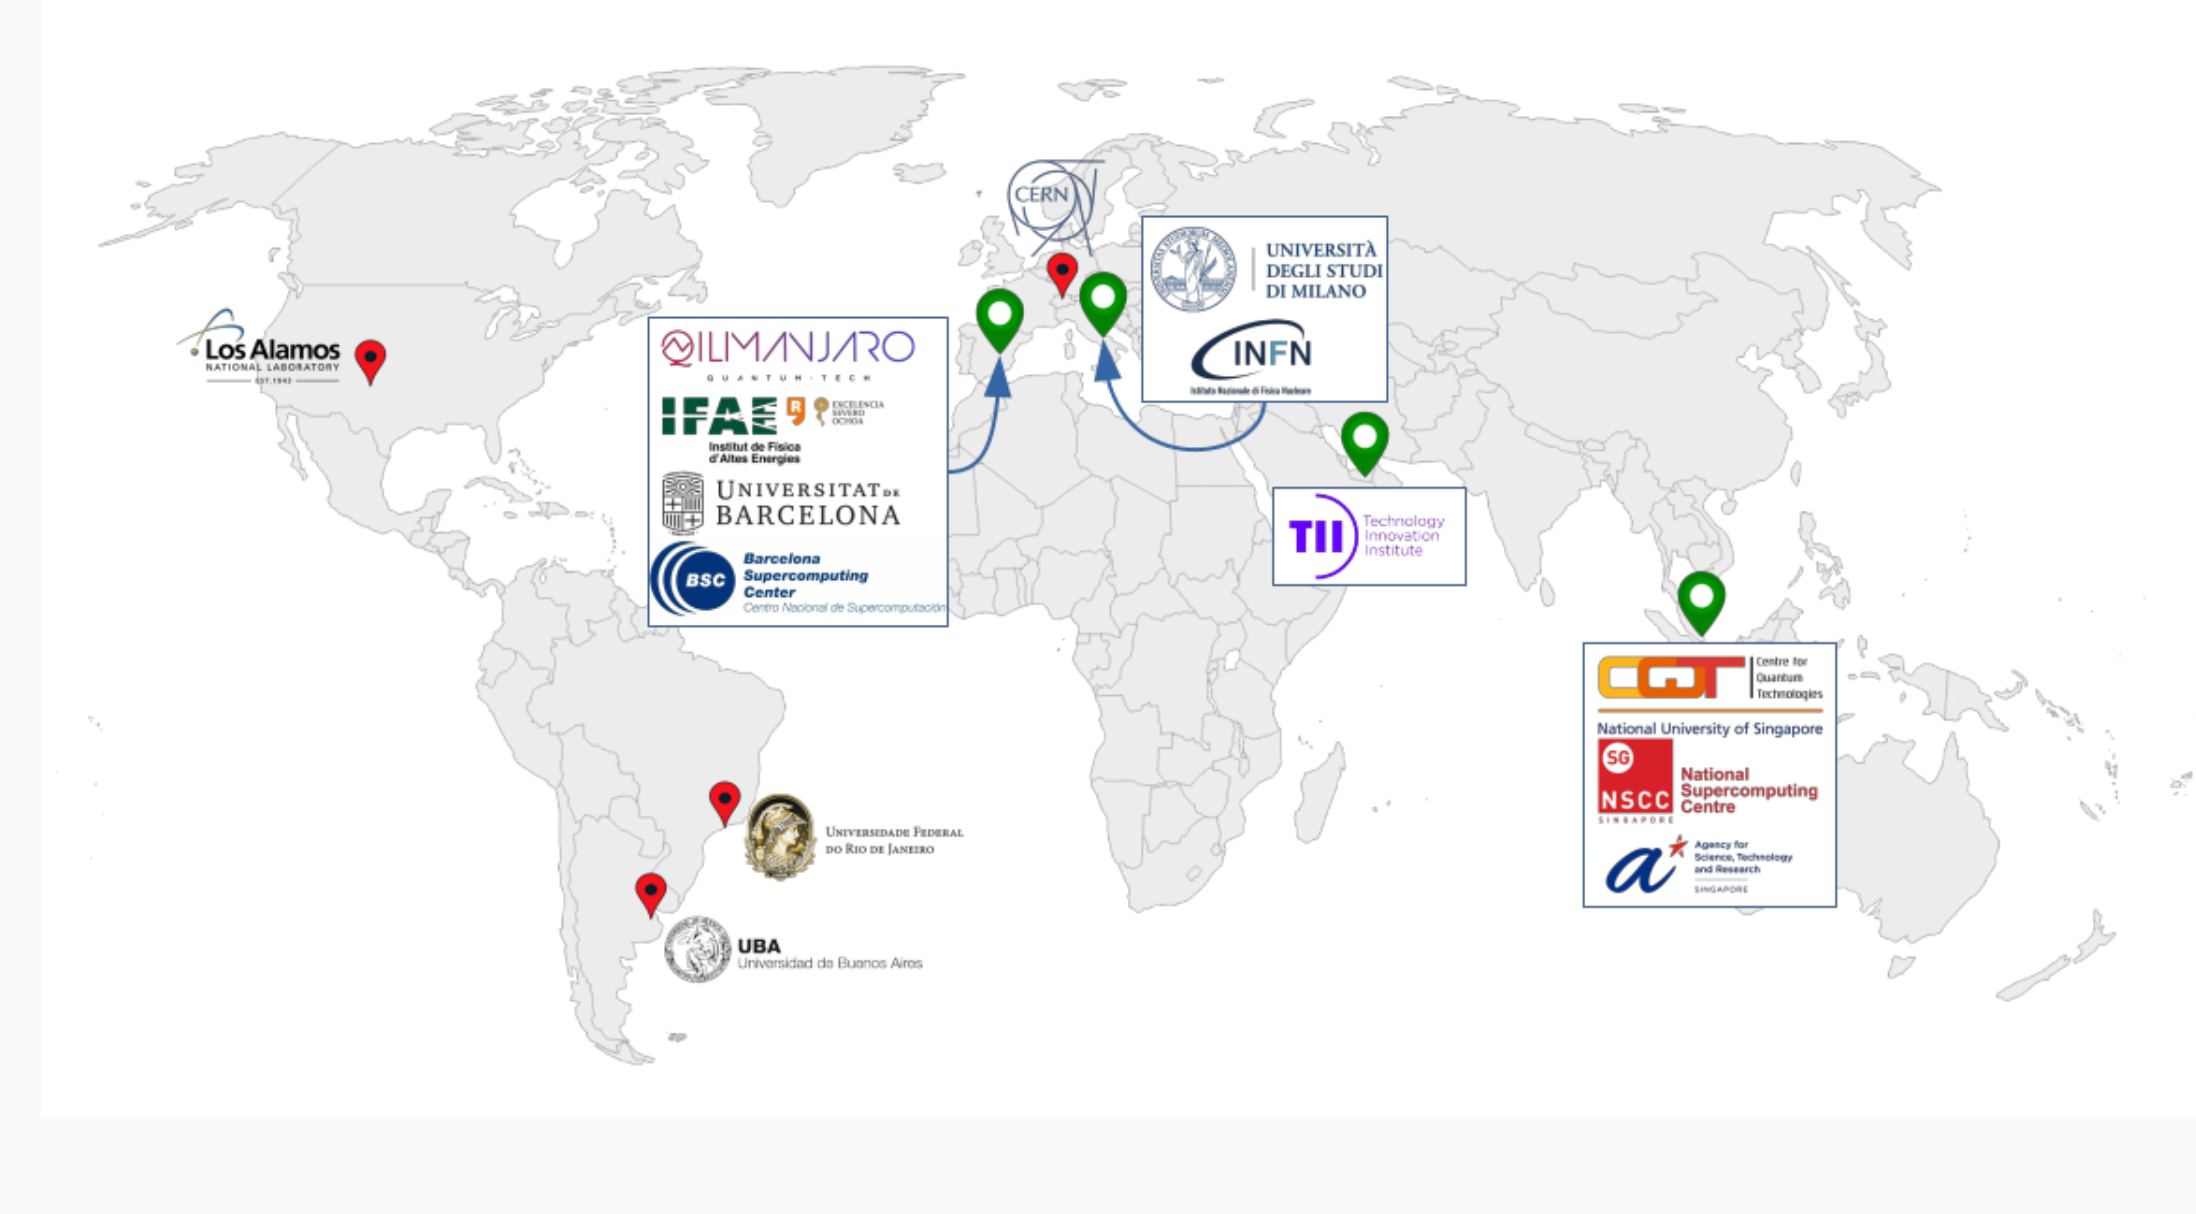
\includegraphics[width=\textwidth]{figures/map.png}
%     \end{figure}
%     % \begin{columns}
%     %     \begin{column}[0.5 \textwidth]
%         \begin{multicols}{2}
%             \begin{itemize}
%                 \item Chips with 1 and 5 qubits at TII
%                 \item Chips with 1 and 2 qubits at Qilimanjaro
%                 \item Chip with 1 qubit in Italy (soon)
%                 \item Chips with up to 10 qubits at CQT
%             \end{itemize}
%         \end{multicols}
%     %     \end{column}
%     %     \begin{column}[0.5 \textwidth]
%     %         test
%     %     \end{column}
%     % \end{columns}
% \end{frame}

\section{Quantum Computing and HPC}

\begin{frame}{Quantum Computing}
    In order to simulate a quantum circuit with $n$ qubits we need to be able to manipulate a $2^n$ components
    vector.

    In Schr\"odinger's approach each gate is applied to the state via the following matrix multiplication
    \begin{equation}\label{eq:gateapplication}
        \psi'(\sigma_1, \ldots, \sigma_n) = \sum _{\boldsymbol{\tau'}} G(\boldsymbol{\tau}, \boldsymbol{\tau'})\psi(\sigma_1,\ldots,\boldsymbol{\tau'},\ldots,\sigma_n)
    \end{equation}
    where the gate targeting $n_{\rm tar}$ qubits is represented by the $2^{n_{\rm
    tar}}\times2^{n_{\rm tar}}$ complex matrix
    $G(\boldsymbol{\tau},\boldsymbol{\tau'})=G(\tau_1,\ldots,\tau_{n_{\rm
    tar}},\tau_1',\ldots,\tau_{n_{\rm tar}}')$ and $\sigma _i, \tau _i\in
    \{0,1\}$.
\end{frame}

\begin{frame}{Example}
\end{frame}


\begin{frame}{What can go wrong?}

    The main issue when building a quantum simulator is the exponential scaling.

    From a coding point of view we need to take care of the following:

    \pause
    \begin{itemize}
        \item Storing in the RAM the state vector
        \pause
        \item Implement efficiently linear algebra operations
    \end{itemize}
    \pause
    Coding a \textbf{good quantum simulator} corresponds to coding a \textbf{good engine} to perfom linear
    algebra operations.

    $\Rightarrow $  HPC comes into play.
    
\end{frame}

\begin{frame}{Challenge}
    \begin{figure}
        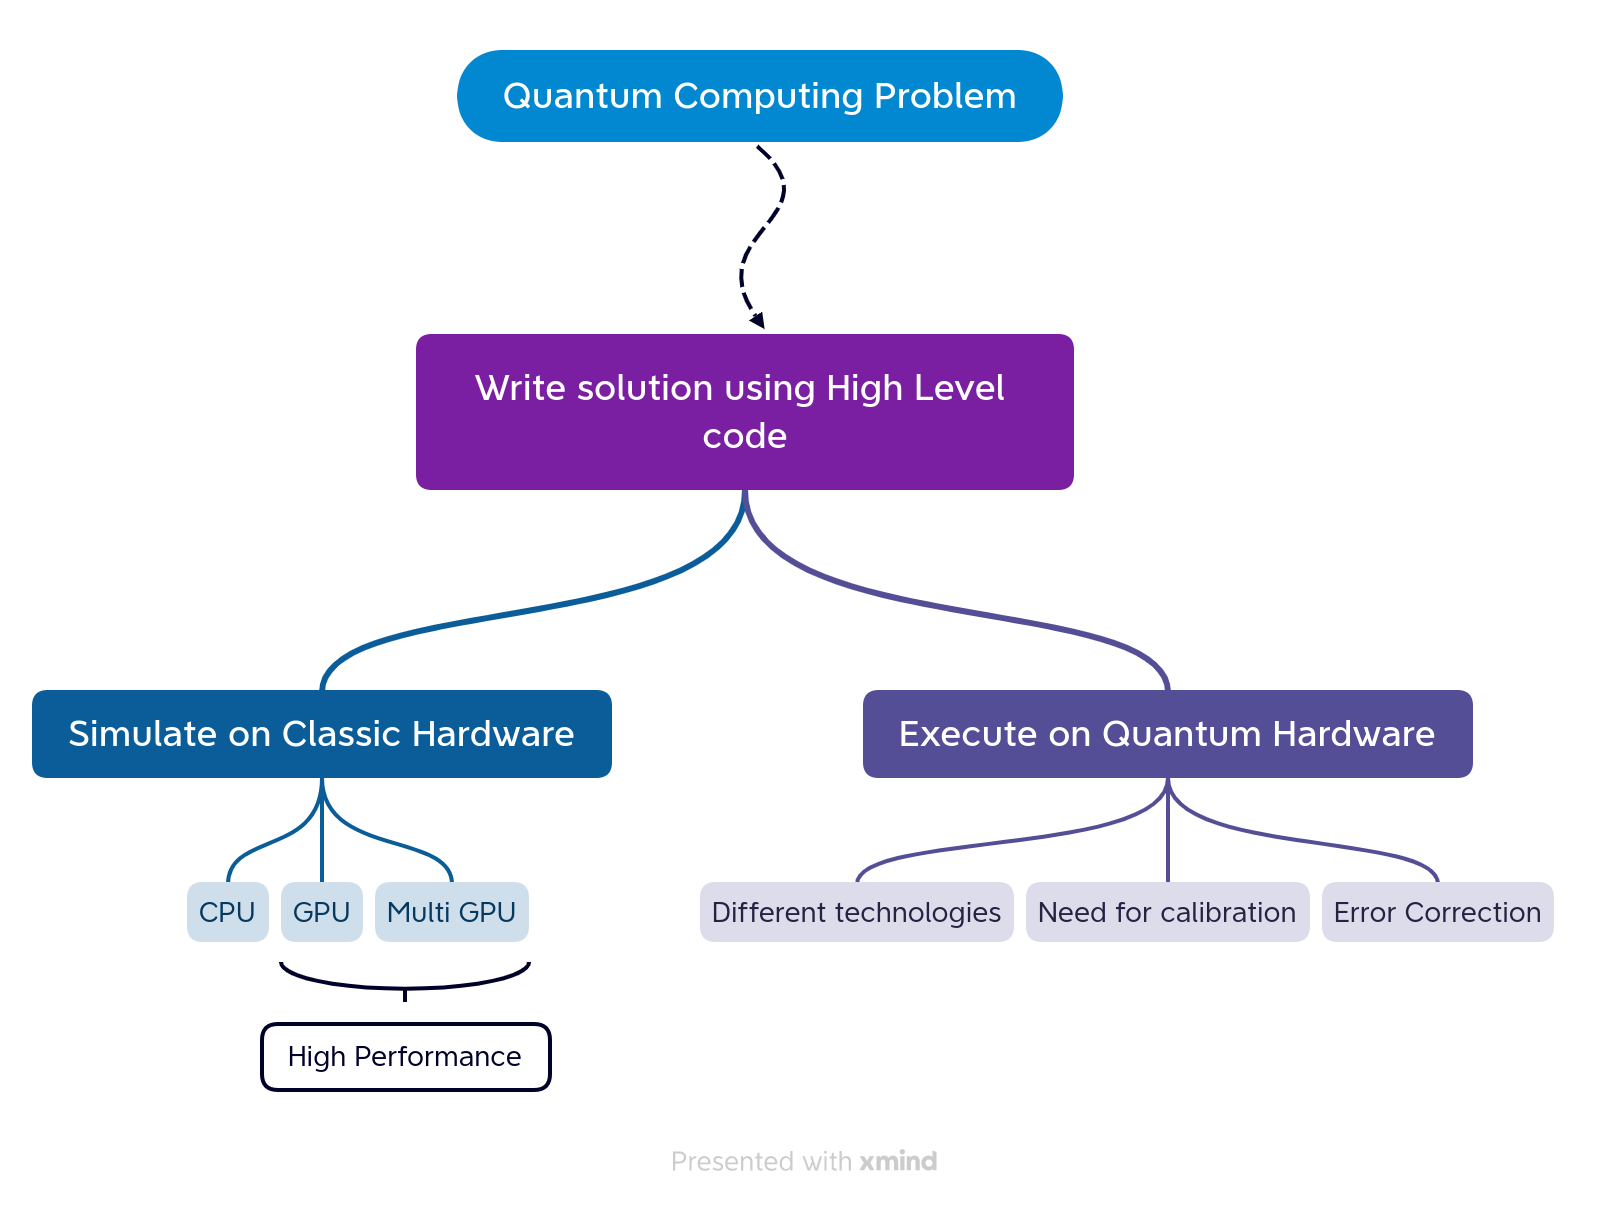
\includegraphics[width=\textwidth]{figures/intro.png}
    \end{figure}
    \centering
    \emph{Is to possible to create from scratch a framework for all of this?}
\end{frame}

\section{Introducing Qibo}

\begin{frame}{Qibo}
    Qibo is an \textbf{open-source} full stack API for \textbf{quantum simulation} and quantum hardware control and calibration.
    \begin{figure}
        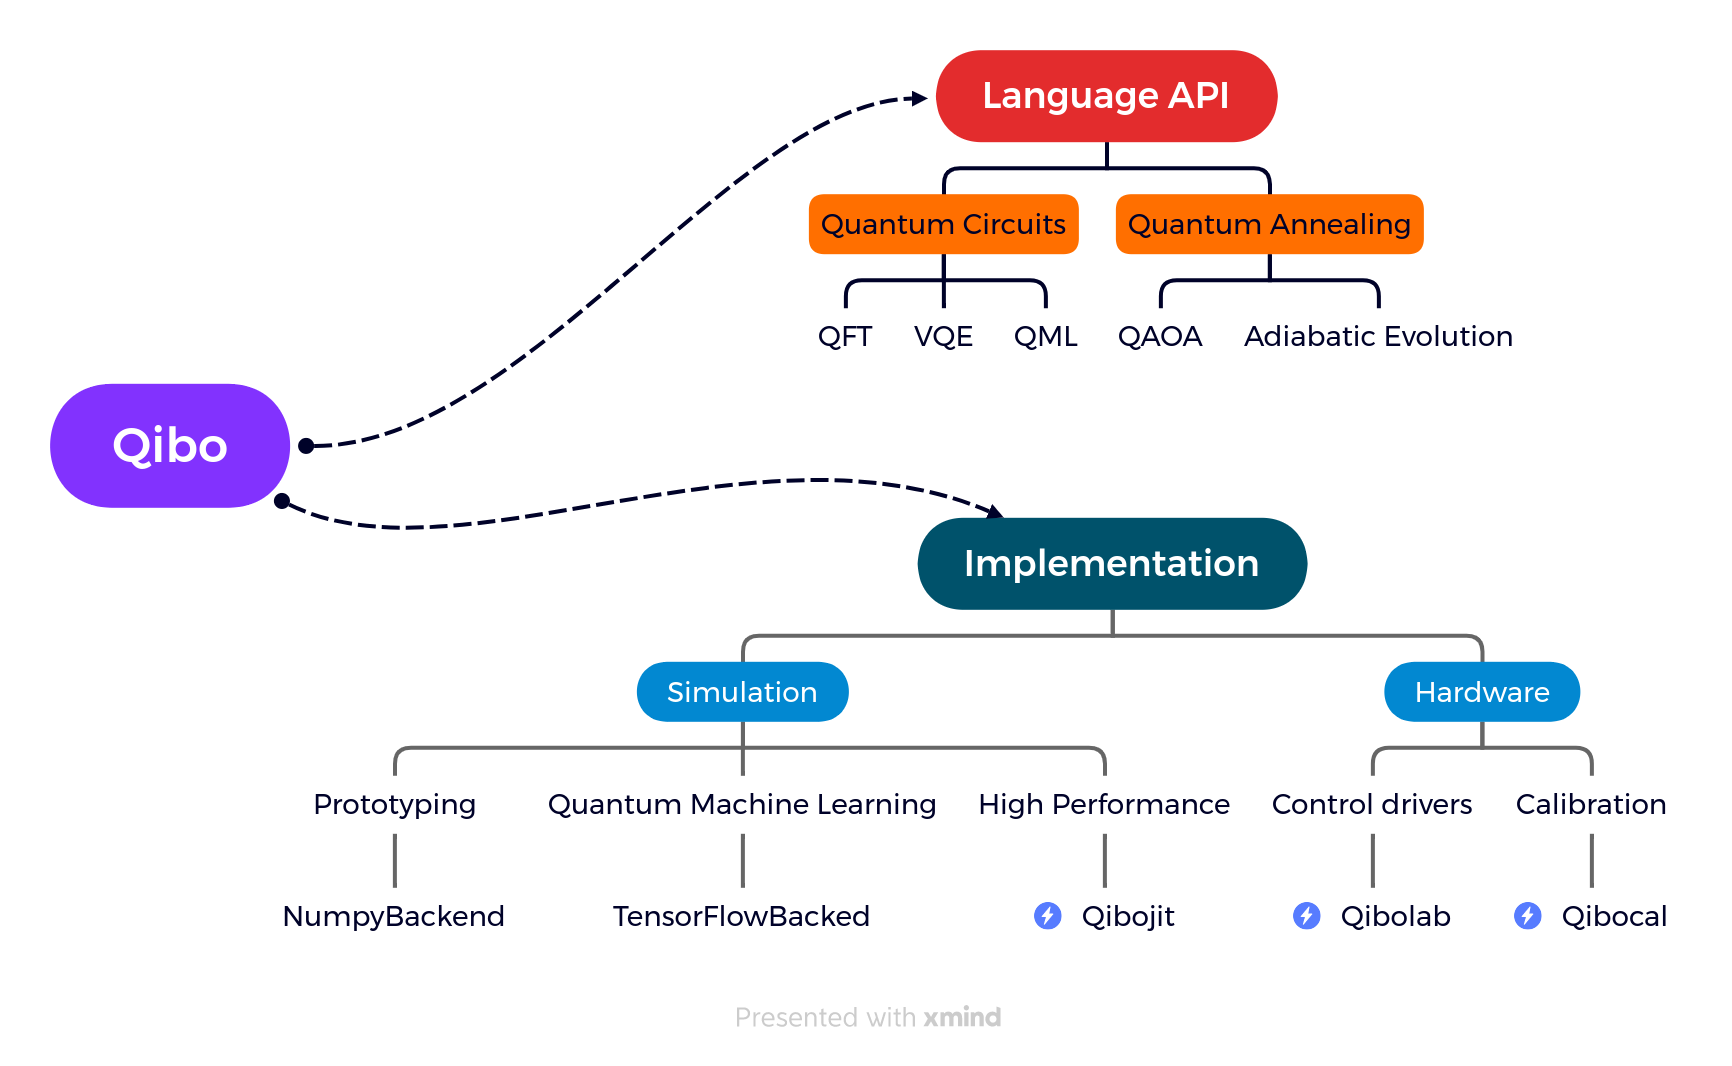
\includegraphics[width= \textwidth]{figures/Qibo.png}
    \end{figure}
    
\end{frame}
% \begin{frame}{A modular framework for quantum computing}
%     \begin{figure}
%         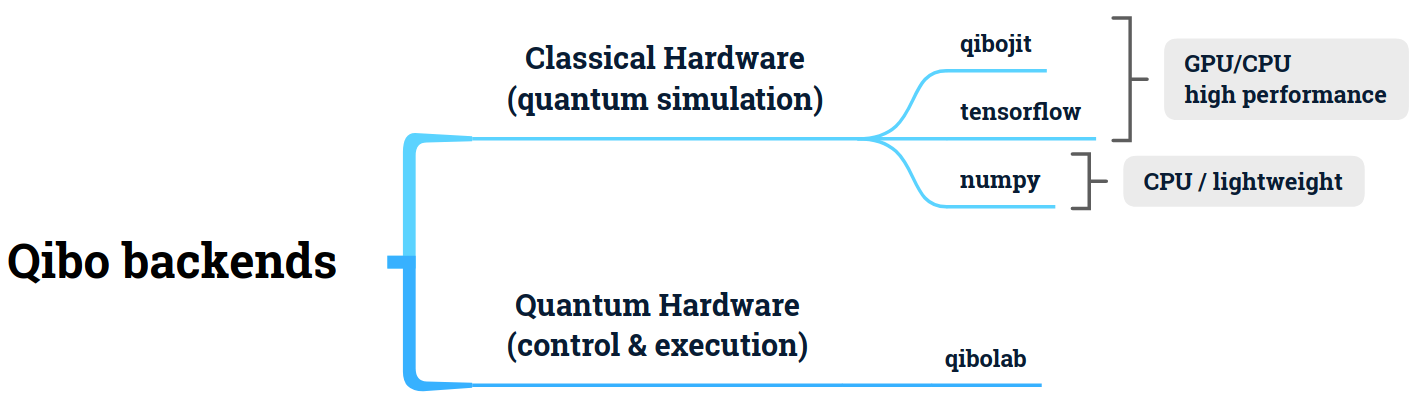
\includegraphics[width= \textwidth]{figures/backends.png}
%     \end{figure}
% \end{frame}

\begin{frame}{Simulation backends in Qibo}
    As already done in many quantum simulation library, Qibo provides multiple backends for
    simulating quantum circuit, i.e. to perform the matrix multiplication of Eq. REF.
    
    The Qibo package is shipped with two basic simulators: \texttt{numpy} and \texttt{tensorflow}.
    
    \begin{columns}
        \begin{column}{0.5 \textwidth}
            \texttt{numpy}
        \end{column}
        \begin{column}{0.5 \textwidth}
            \texttt{tensorflow}
        \end{column}
    \end{columns}
\end{frame}

% \begin{frame}{Introducing Qibojit}
%     Matrix multiplication to simulate circuits:

%     \begin{equation*}\label{eq:gateapplication}
%         \psi'(\sigma_1, \ldots, \sigma_n) = \sum _{\boldsymbol{\tau'}} G(\boldsymbol{\tau}, \boldsymbol{\tau'})\psi(\sigma_1,\ldots,\boldsymbol{\tau'},\ldots,\sigma_n) \ .
%     \end{equation*}

    
    
%     { \color{red} \faClose}  Number of operations scales { \color{red} exponentially} with the number of qubits!
   
%     We need more sophisticated backends to perform simulation:
%     \begin{itemize}
%         \item[{ \color{red} \faClose}] \texttt{NumpyBackend} : { \color{blue} Numpy} tensors and primitives
%         \item[{ \color{red} \faClose}] \texttt{TensorFlowBackend} : { \color{orange} Tensorflow} tensors and primitives
%         \item[{ \color{green} \faCheck}] \texttt{QibojitBackend} : Just-In-time
%         \item[]     \begin{itemize}
%             \item[\faCode] CPU : { \color{blue} Numpy} tensor + custom operations with {\color{cyan} Numba JIT}
%             \item[\faCode] GPU(S) : {\color{teal} Cupy} tensors + custom operations using
%             \begin{itemize}
%                 \item  {\color{teal} Cupy JIT} Raw kernels
%                 \item  {\color{green} NVIDIA cuQuantum}  API
%             \end{itemize} 
%         \end{itemize}
%     \end{itemize}

%     Paper published on Quantum: \url{https://quantum-journal.org/papers/q-2022-09-22-814/}

    
% \end{frame}

\begin{frame}{Numpy Backend}
    \begin{multicols*}{2}
        Simulator based on \texttt{numpy}:
        \begin{itemize}
            \item \texttt{np.ndarray}
            \item \texttt{numpy} primitives 
        \end{itemize}
        \begin{figure}
            
\includegraphics[width=0.3 \textwidth]{figures/numpy.png}
        \end{figure}
    \end{multicols*}
    
    
    \textbf{FEATURES}
    \begin{multicols*}{2}
        \begin{itemize}
            \item Cross-architecture (x86, arm64, etc)
            \item Cross-platform
            \item Fast for small circuits
            \item Fast for single-threaded operations
        \end{itemize}
    \end{multicols*}

    
\end{frame}

\begin{frame}{TensorFlow Backend}

    \begin{multicols*}{2}
        Simulator based on \texttt{tensorflow} primitives:
    \begin{itemize}
        \item \texttt{tf.Tensor}
        \item  \texttt{tf.matmul} and \texttt{tf.matmul}
    \end{itemize}
    \begin{figure}
        
\includegraphics[width=0.3 \textwidth]{figures/tensorflow.jpg}
    \end{figure}
    \end{multicols*}
    

    \textbf{FEATURES}
    \begin{multicols*}{2}
        \begin{itemize}
            \item Multithreading CPU
            \item Single GPU
            \item Gradient descent on quantum circuits
            \item QML using Qibo
        \end{itemize}
    \end{multicols*}
    
\end{frame}

\begin{frame}{Performance}
    \begin{figure}
        \centering
        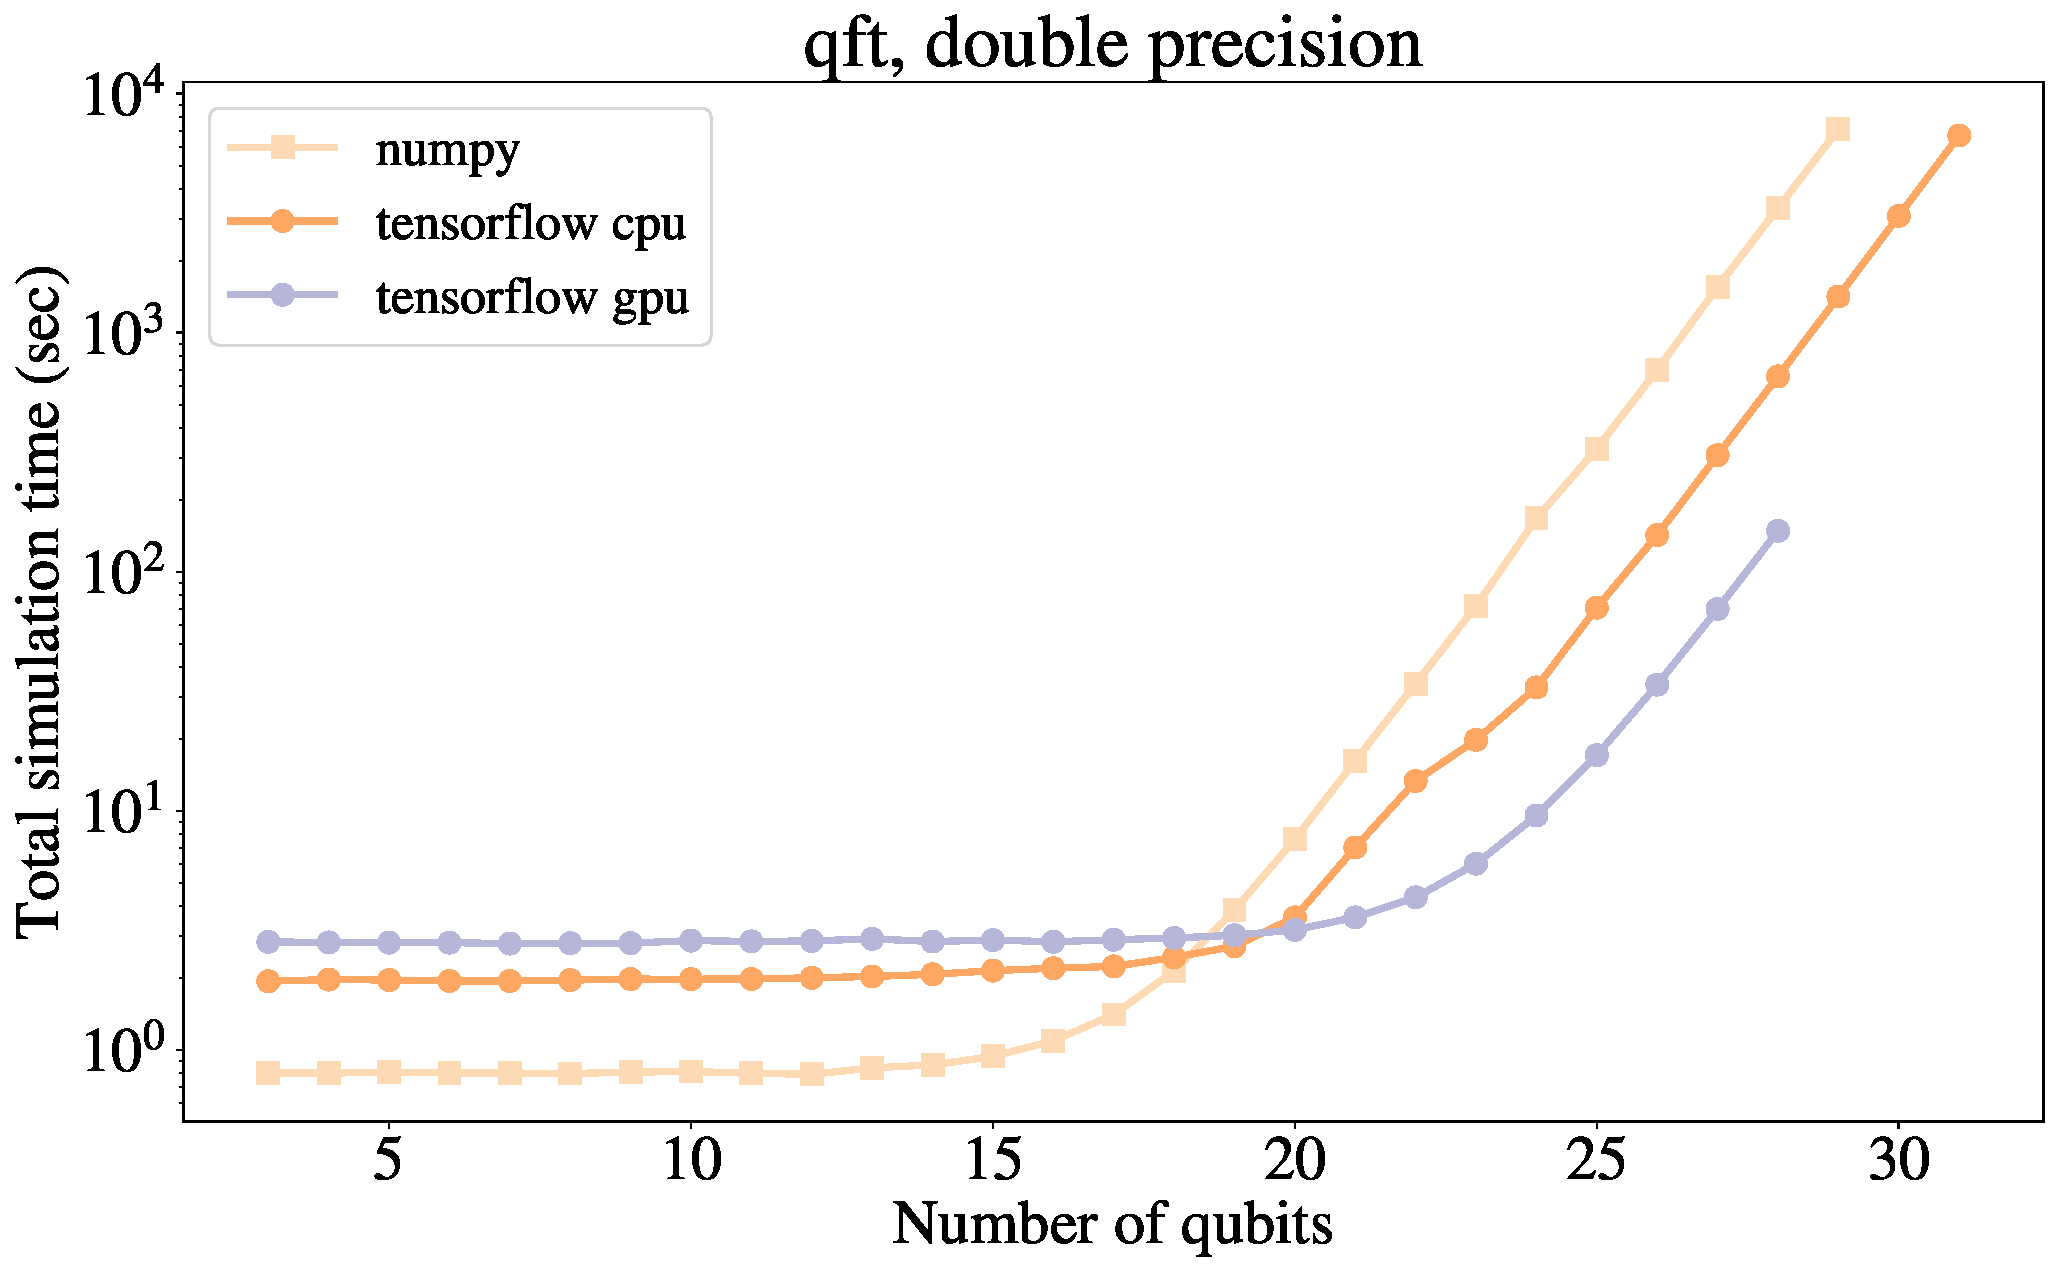
\includegraphics[width=0.7\textwidth]{figures/np_tf_double.pdf}
    \end{figure}

    \begin{multicols*}{2}
        \begin{itemize}        
        \item Increasing the computational times
        \item Tensorflow better than numpy
        \item GPU helps!
    \end{itemize}
    \end{multicols*}

\end{frame}

\begin{frame}{Can we do better than this?}
    To efficiently simulate circuits with large number of qubits we designed
    a new backend \textbf{qibojit}.


    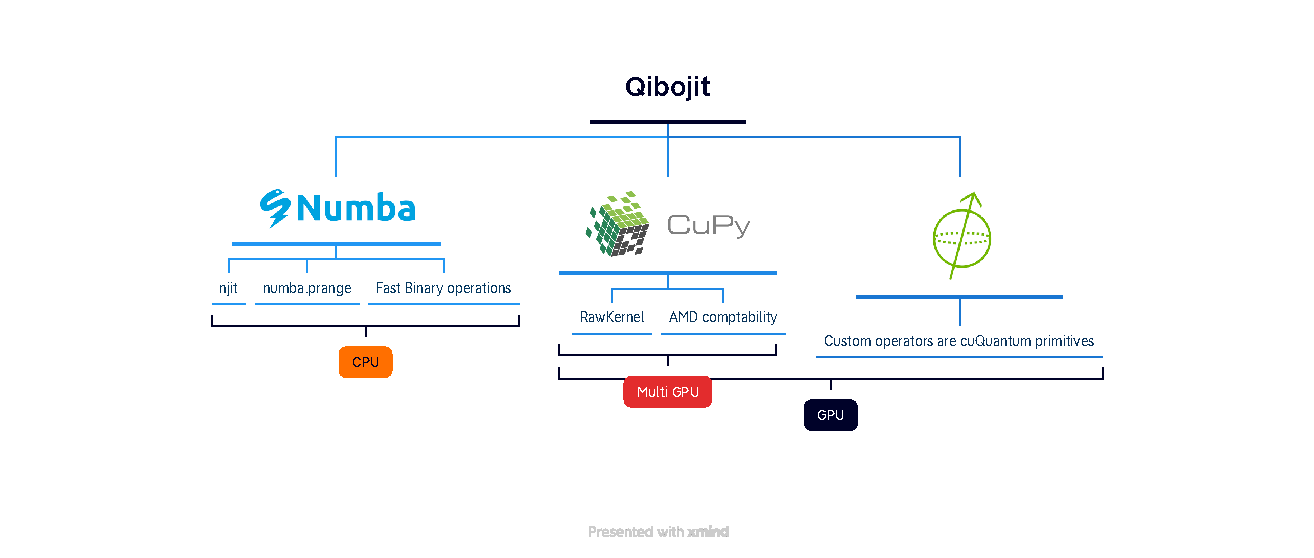
\includegraphics[width=\textwidth]{figures/Qibojit.pdf}
    
    \textbf{FEATURES}
    \begin{multicols*}{2}
        \begin{itemize}
            \item \emph{in-place} updates 
            \item exploit \emph{sparsity of matrix}
            \item Just-in-Time compilation
            \item CuQuantum compatibility
        \end{itemize}
    \end{multicols*}

\end{frame}

\begin{frame}{What is Just-in-Time (JIT) compilation?}

    JIT: a method for improving the performance of interpreted programs.

    \textbf{Static compiler}: reads a programme, looks at the code and tries 
    to convert it into machine code

    \textbf{Interpreter}: looks at the programme, does not convert to machine
    code and it execute it almost as it is

    \textbf{Just-in-Time compiler}: starts a programme running an interpreter
    and dynamically produce machine code based on the observation of the programme

    JIT compilers can be \textbf{faster} than a static compiler because they can get
    more information by running the programme instead of just looking at the
    programme at compile time! 

    INTRODUCE DRY RUN vs SIMULATION TIME

    
\end{frame}

\begin{frame}{Numba example}
    \begin{figure}
        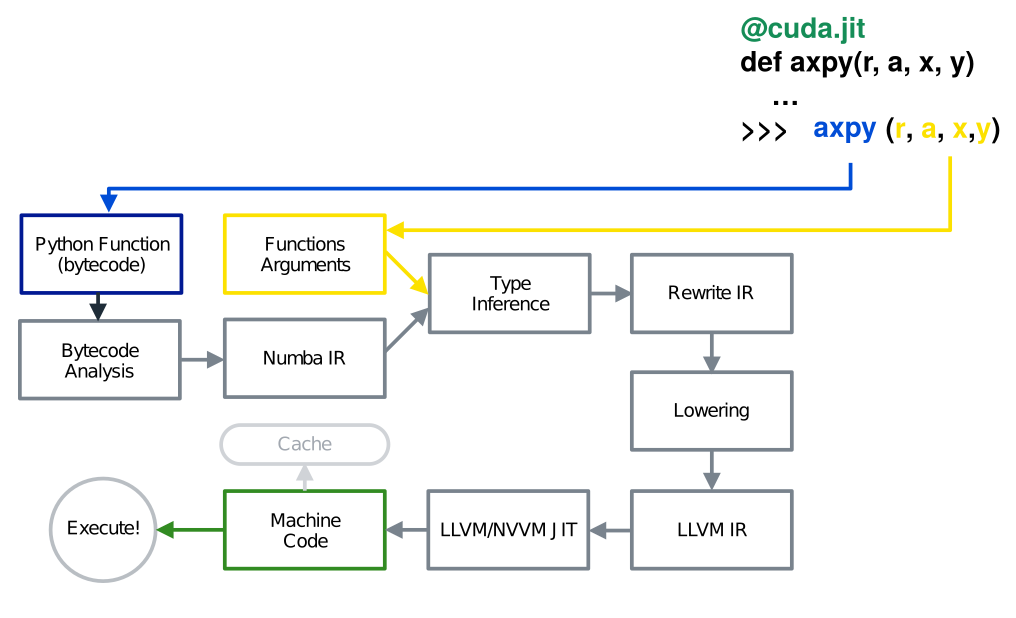
\includegraphics[width= \textwidth]{figures/how_numba.png}
    \end{figure}
    
\end{frame}


\begin{frame}[fragile]{Qibojit - Example}

    \begin{columns}
        \begin{column}{0.7\textwidth}
            \hspace{1cm}
            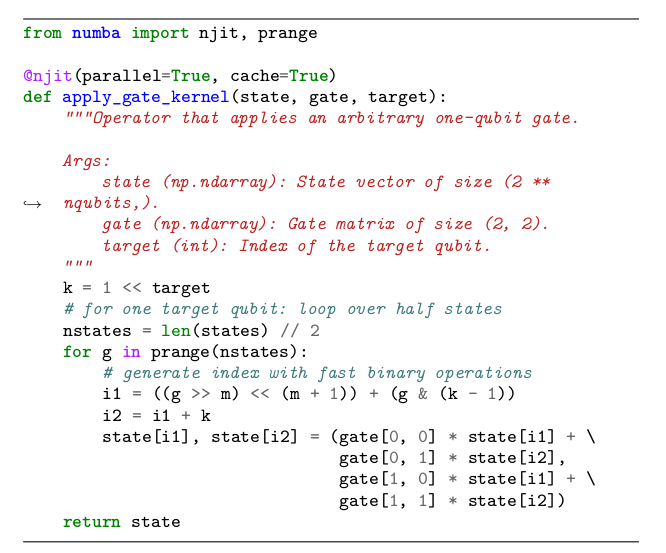
\includegraphics[width = 0.8\textwidth]{figures/circuit.png}
        \end{column}

        \begin{column}{0.6\textwidth}
            Observations
            \begin{itemize}
                \item \texttt{@njit}
                \item \texttt{prange}
                \item fast binary operations
            \end{itemize}
        \end{column}
    \end{columns}

    
\end{frame}

\begin{frame}{Qibojit GPU backends : Cupy}
    Same approach followed using Numba: JIT compilation.

    Custom operators implemented using \texttt{cupy.RawKernel}:
    \begin{enumerate}
        \item Write custom CUDA kernels written in C++
        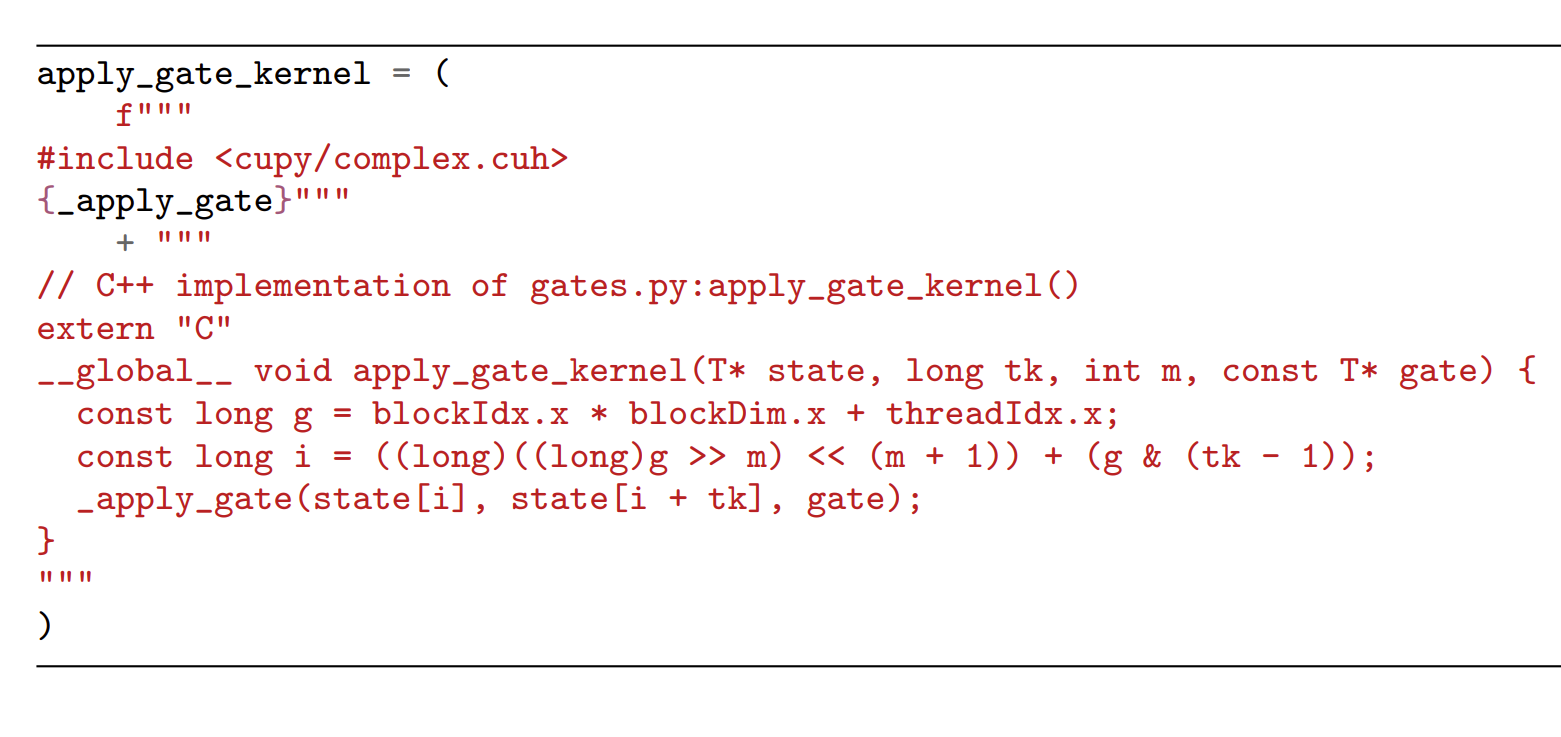
\includegraphics[width = 0.6 \textwidth]{figures/cupy.png}
        \item At the first invocation the kernel will be compiled using nvcc
        \item After the first invocation it is cached for each device
    \end{itemize}

\end{frame}

\begin{frame}{CuQuantum Backend}
    Writing custom operators takes time and efforts and can be highly non-trivial.
    Instead of writing the custom operators yourself the modular layout of Qibo
    enable the user to write its custom backend.

    \begin{figure}
        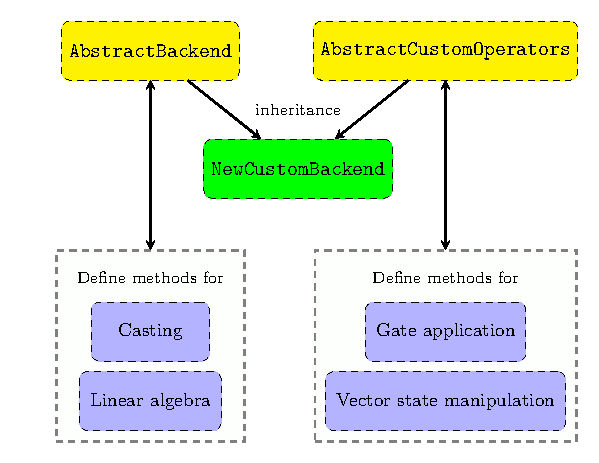
\includegraphics[width= 0.6 \textwidth]{figures/backend_implementation.pdf}
    \end{figure}
    
    First successful application: CuQuantum Backend.

\end{frame}

\begin{frame}{Nvidia CuQuantum}
    cuQuantum has a Python API which delivers all the functionalities 
    \texttt{cuStateVec} and \texttt{cuTensorNet} with Python API.

    Starting from the \texttt{Cupy} we replaced the custom operators with CuQuantum
    primitives.

    The compatibility with Cupy allows to fallback of the custom operators
    of the \texttt{CupyBackend} to mantain good performance without complicating the code.

\end{frame} 
\begin{frame}{Benchmarks}
    \begin{figure}
        % 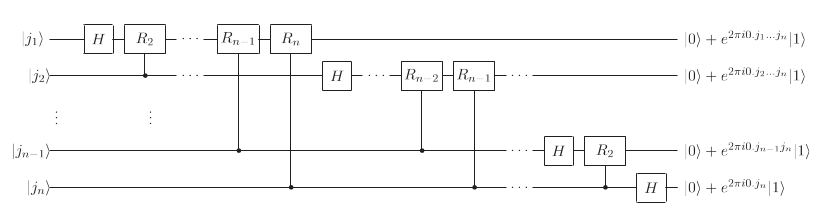
\includegraphics[width=0.8 \textwidth]{figures/qft.png}
        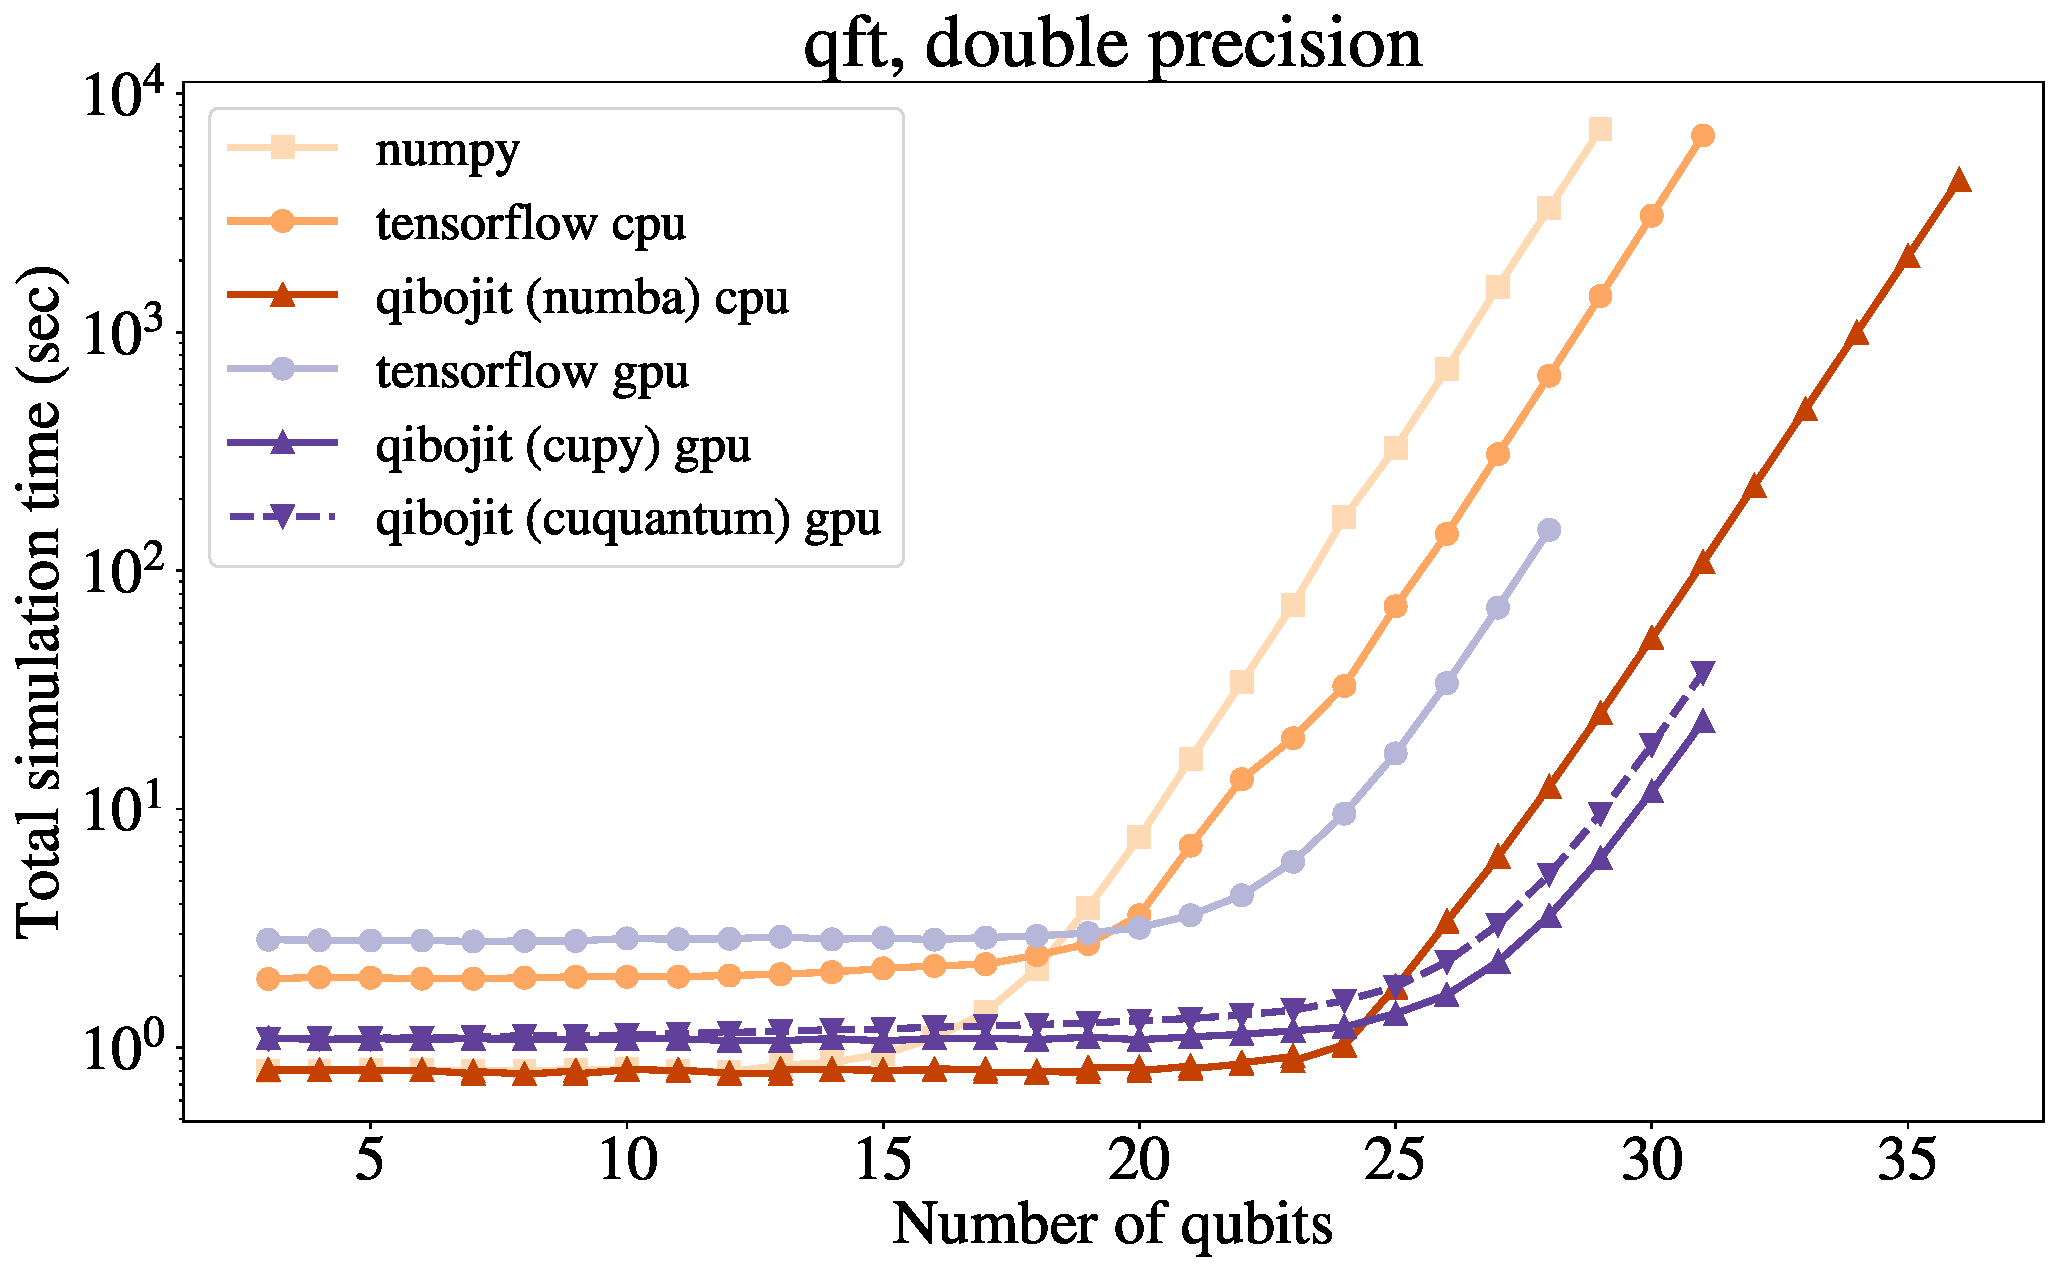
\includegraphics[width=0.8 \textwidth]{figures/qibo_scaling_qft_total_simulation_time_double.pdf} 
    \end{figure}
    Benchmark library: \url{https://github.com/qiboteam/qibojit-benchmarks}
\end{frame}

\begin{frame}{Benchmark on different devices}

            \begin{figure}
                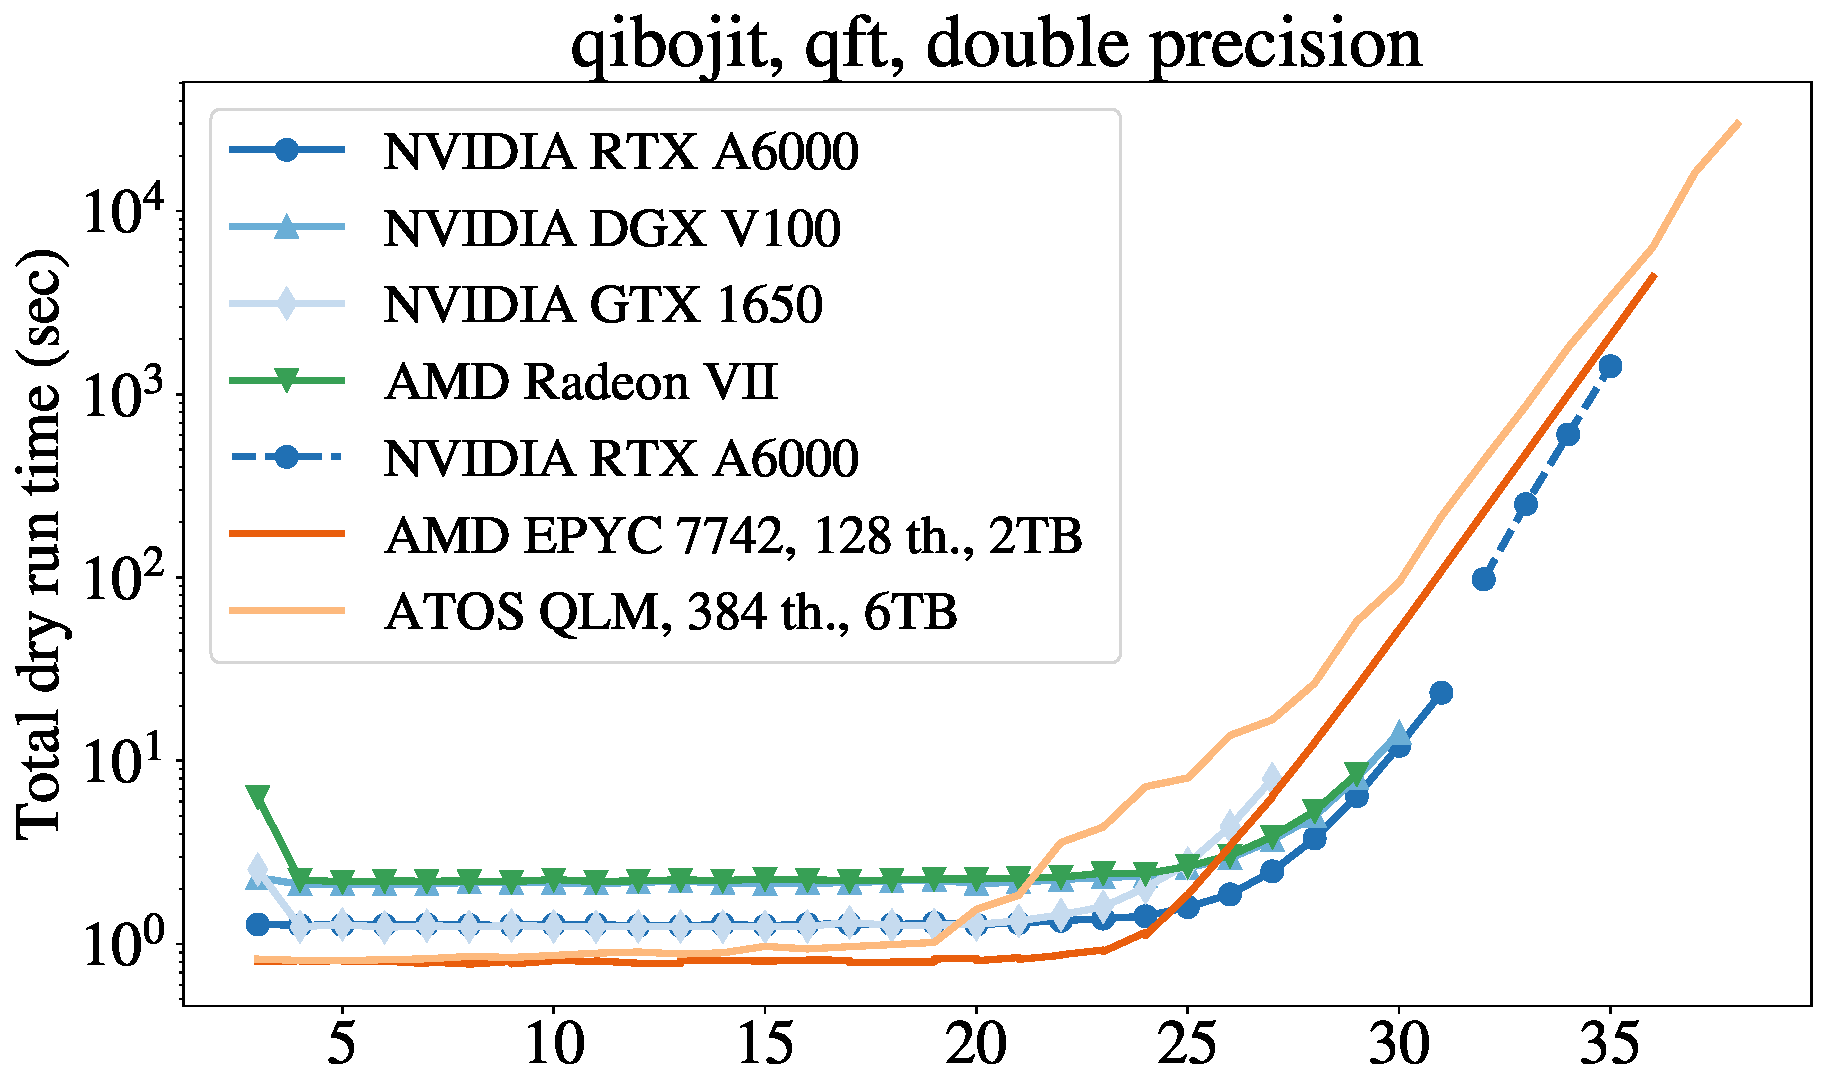
\includegraphics[width = 0.5 \textwidth]{figures/devices_qft_total_dry_time_double.pdf}
                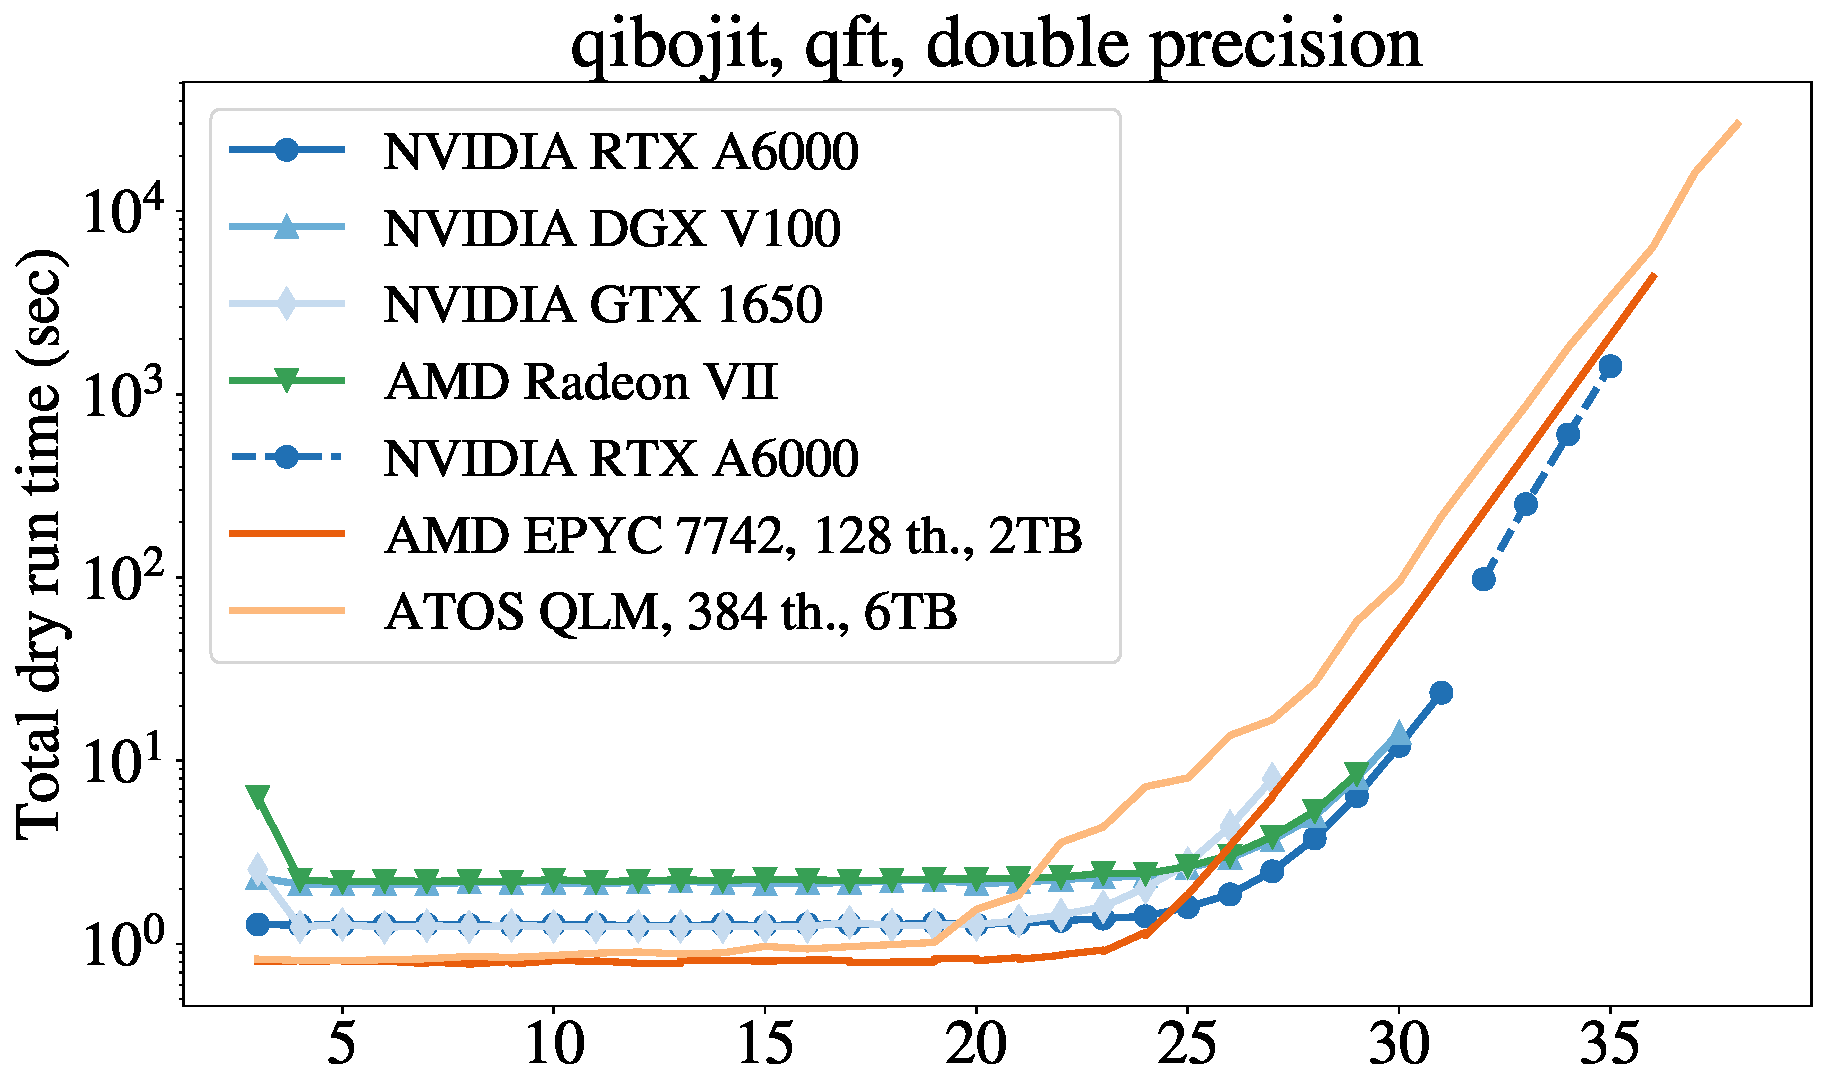
\includegraphics[width = 0.5 \textwidth]{figures/devices_qft_total_simulation_time_double.pdf}
            \end{figure}
    
\end{frame}

\begin{frame}{Multi-GPU support}
    \texttt{CupyBackend} supports also multi-GPU architectures

    \begin{figure}
        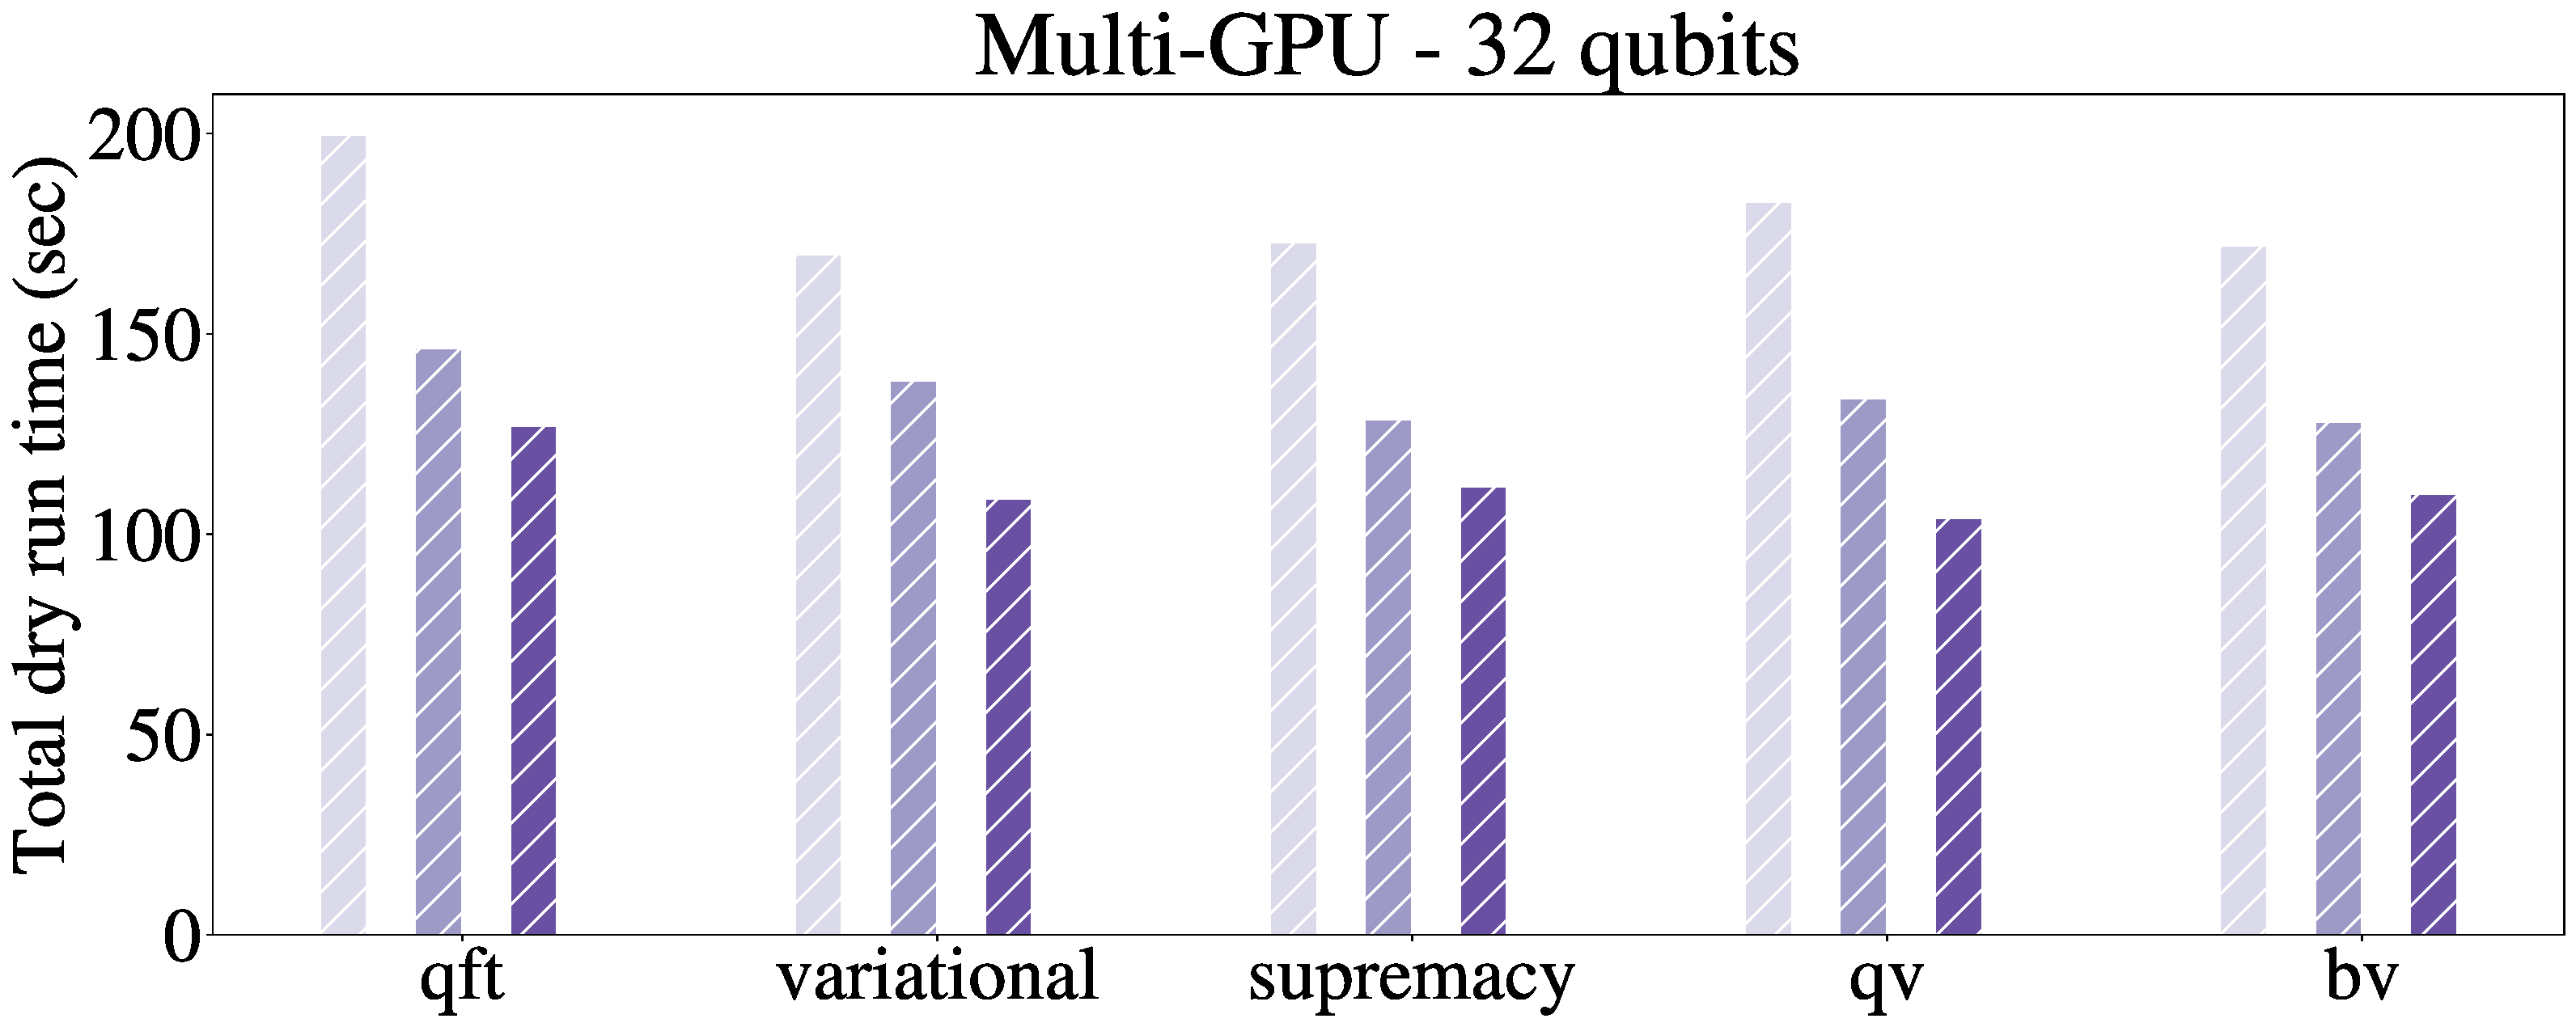
\includegraphics[height= 0.4 \textheight]{figures/multigpu_32qubits_total_dry_time_double.pdf}
        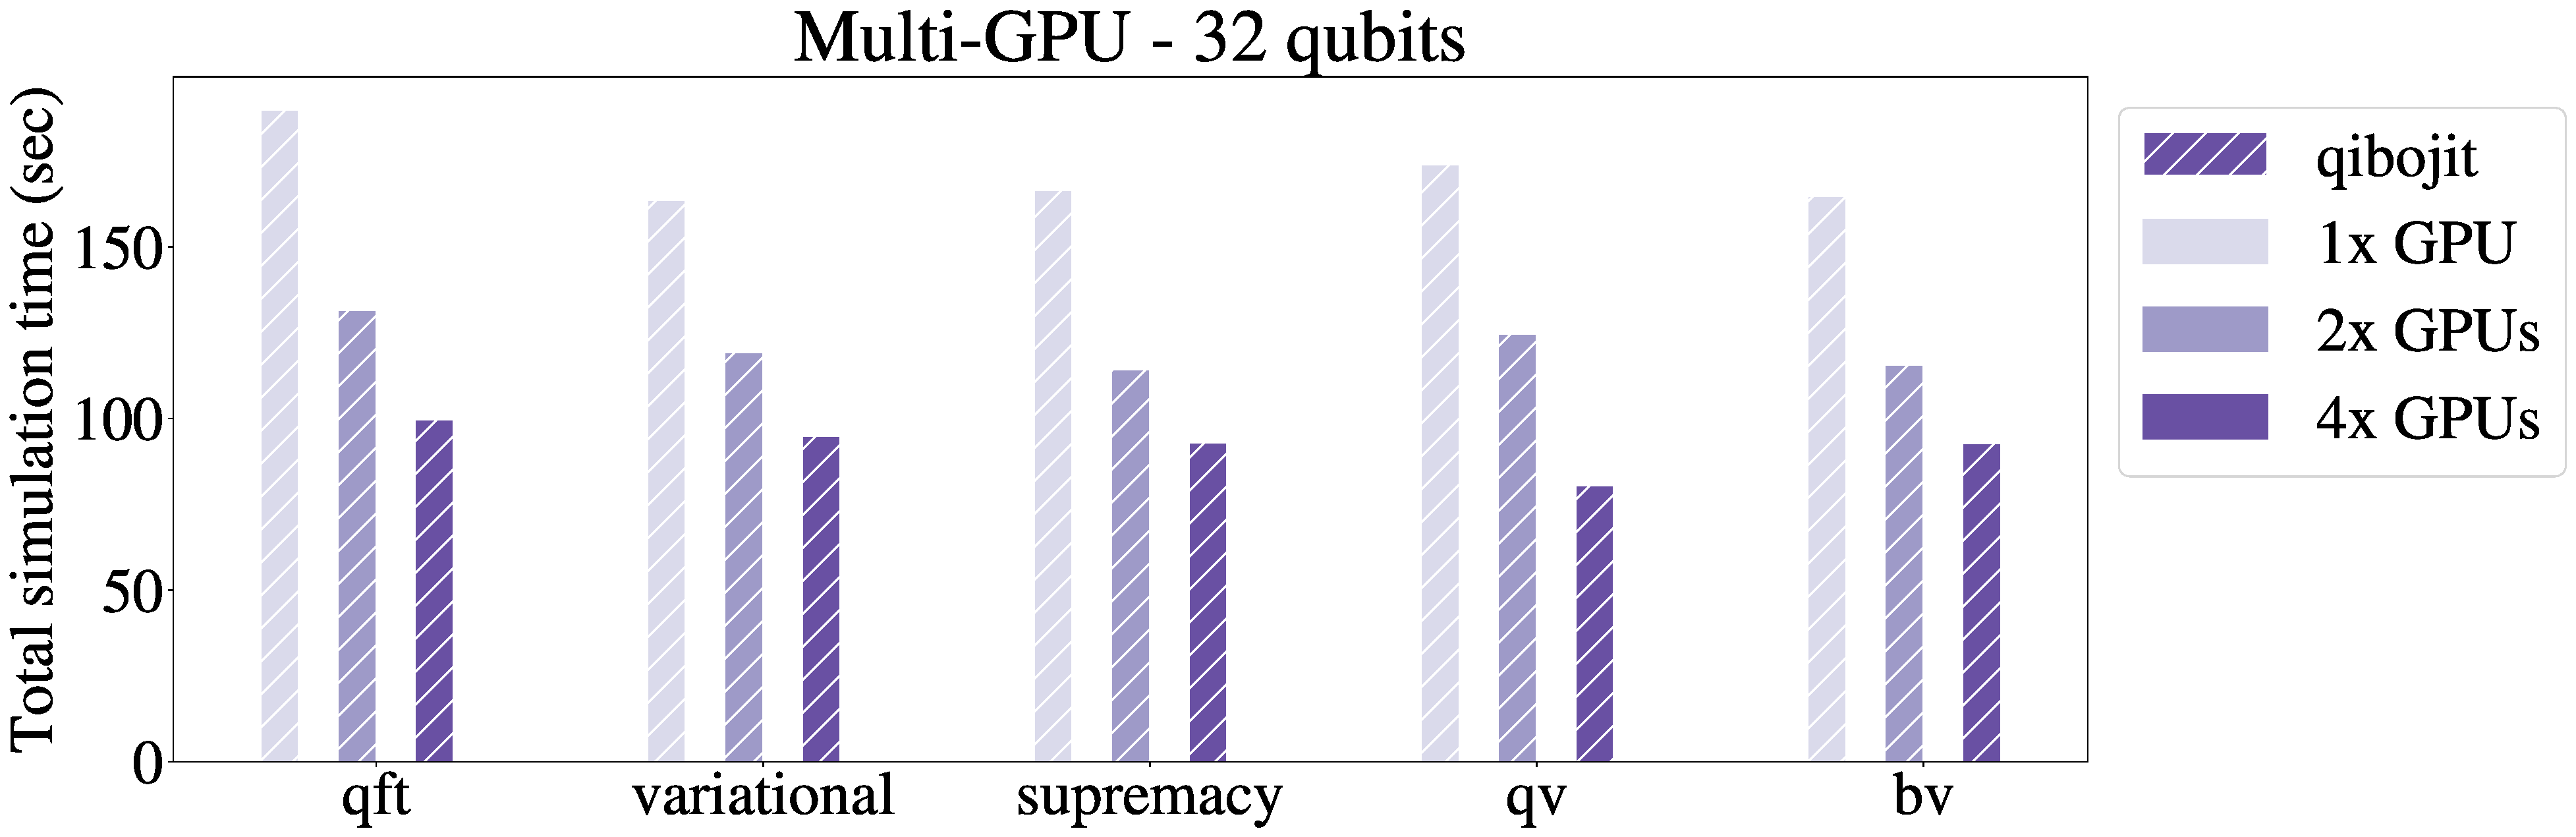
\includegraphics[height= 0.315 \textheight]{figures/multigpu_32qubits_total_simulation_time_double.pdf}
    \end{figure}
\end{frame}

% \begin{frame}{Benchmarks}
%     \begin{columns}
%         \begin{column}{0.8 \textwidth}

%             % \begin{figure}[ht]
%             %     \fbox{\begin{minipage}[t]{0.8 \textwidth}
%             %       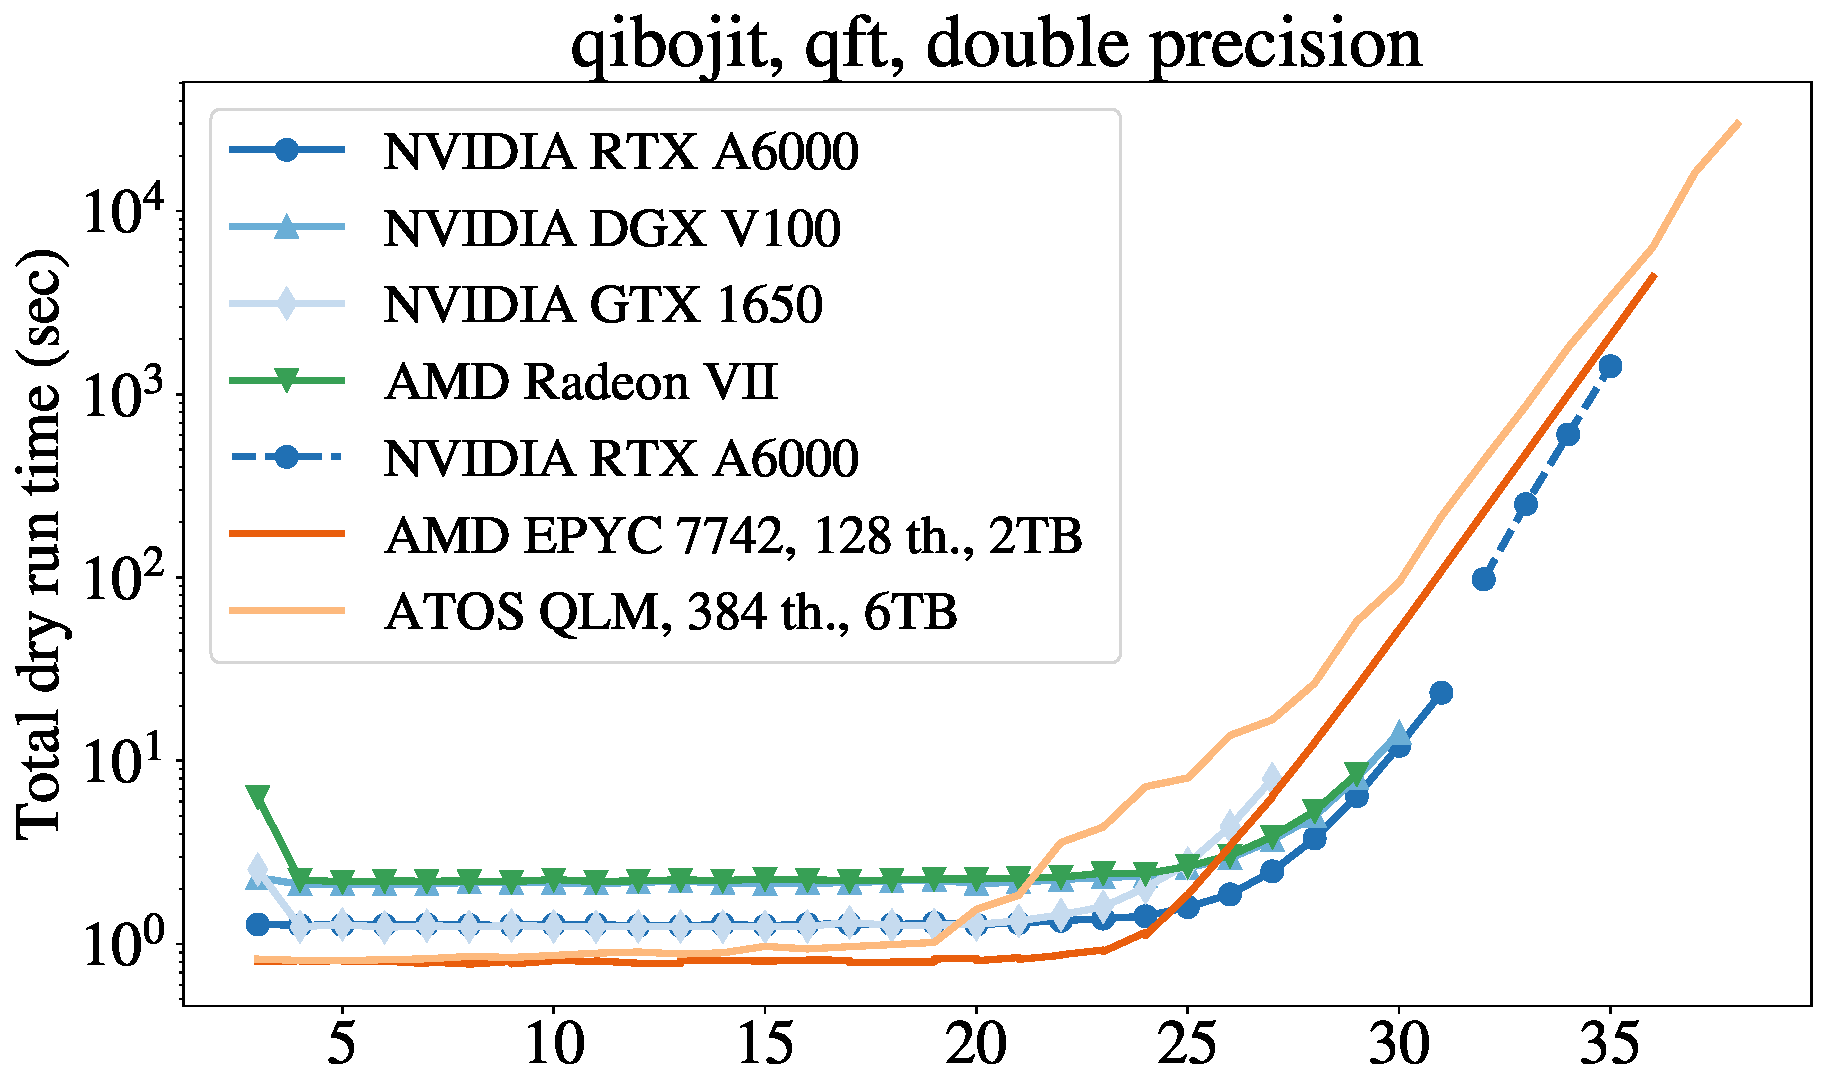
\includegraphics[width=0.8 \textwidth]{figures/devices_qft_total_simulation_time_double.pdf}
%             %     \end{minipage}}
%             %     \hfill
%             %     \fbox{\begin{minipage}[t]{0.8 \textwidth}
%             %       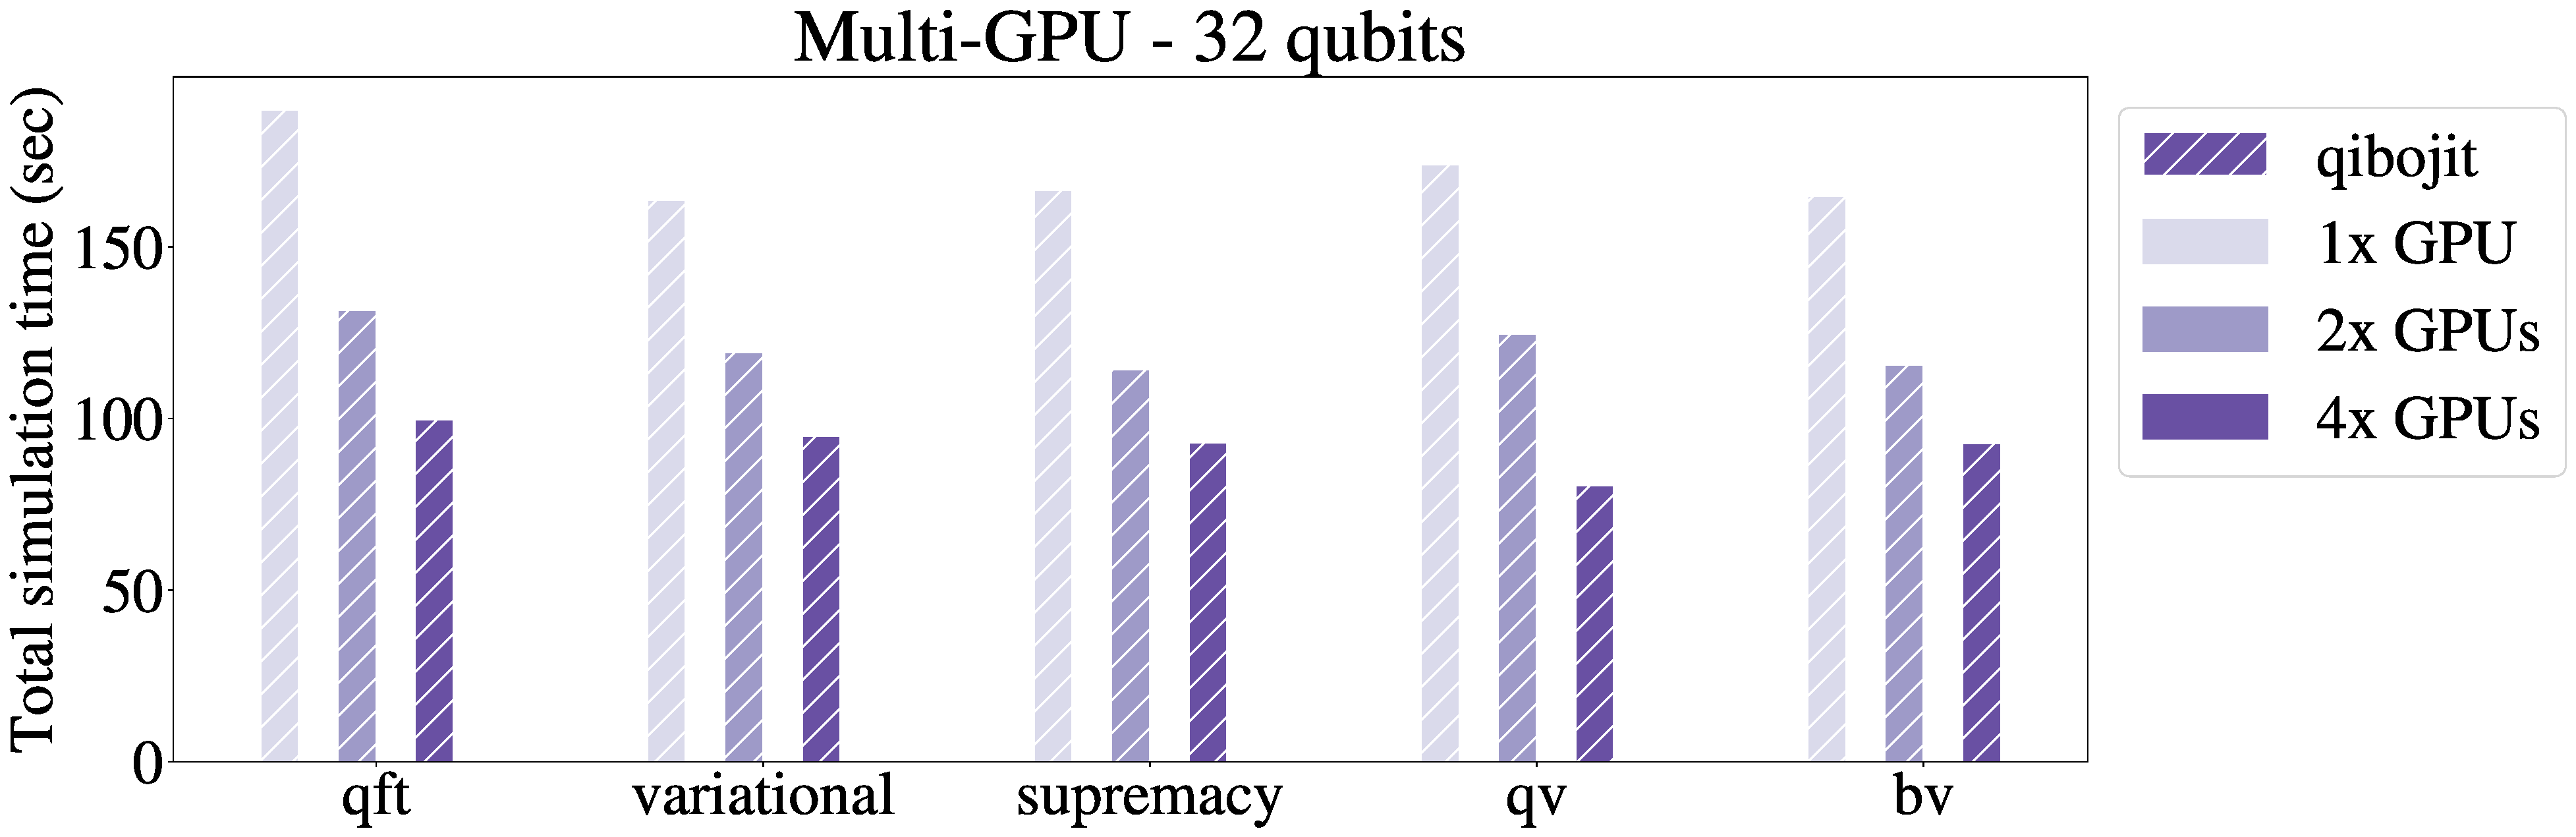
\includegraphics[width=0.8 \textwidth]{figures/multigpu_32qubits_total_simulation_time_double.pdf}
%             %     \end{minipage}}
%             %   \end{figure}
%             \begin{figure}
%             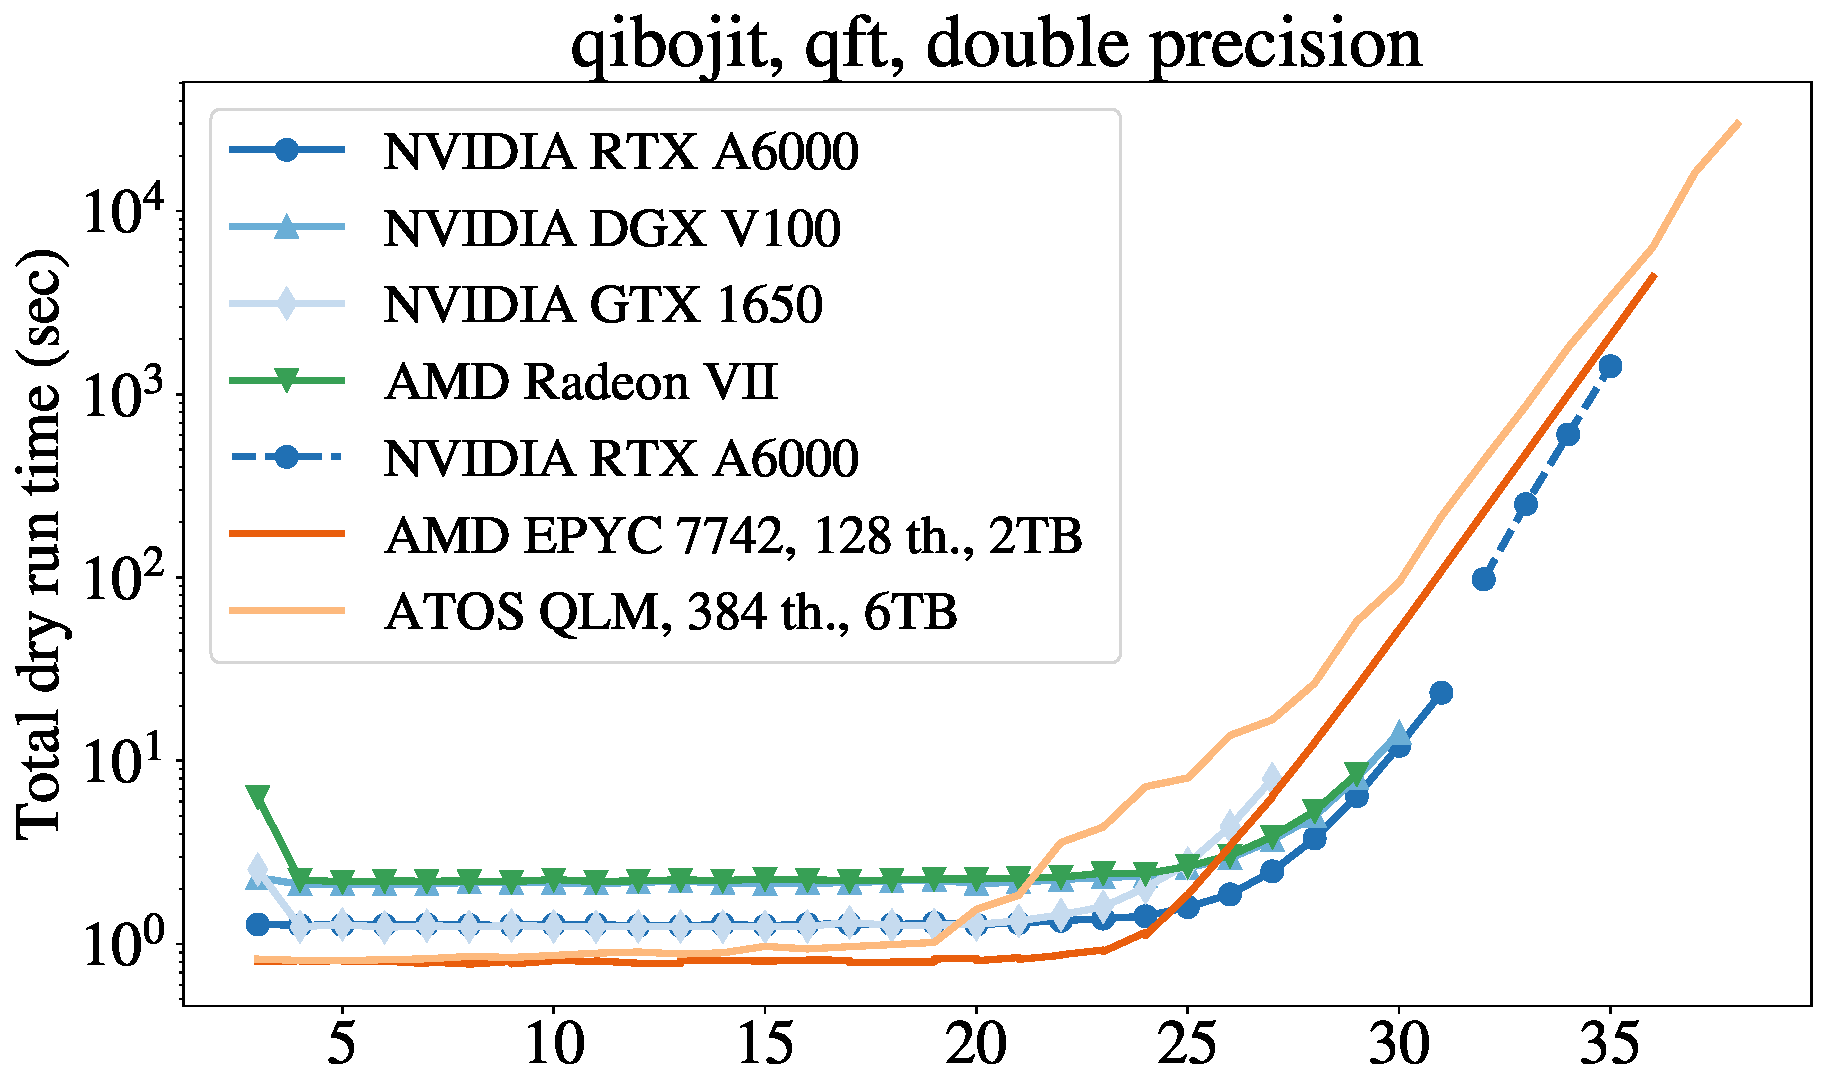
\includegraphics[width=0.8 \textwidth]{figures/devices_qft_total_simulation_time_double.pdf}
%             \hspace{0.5cm}

%             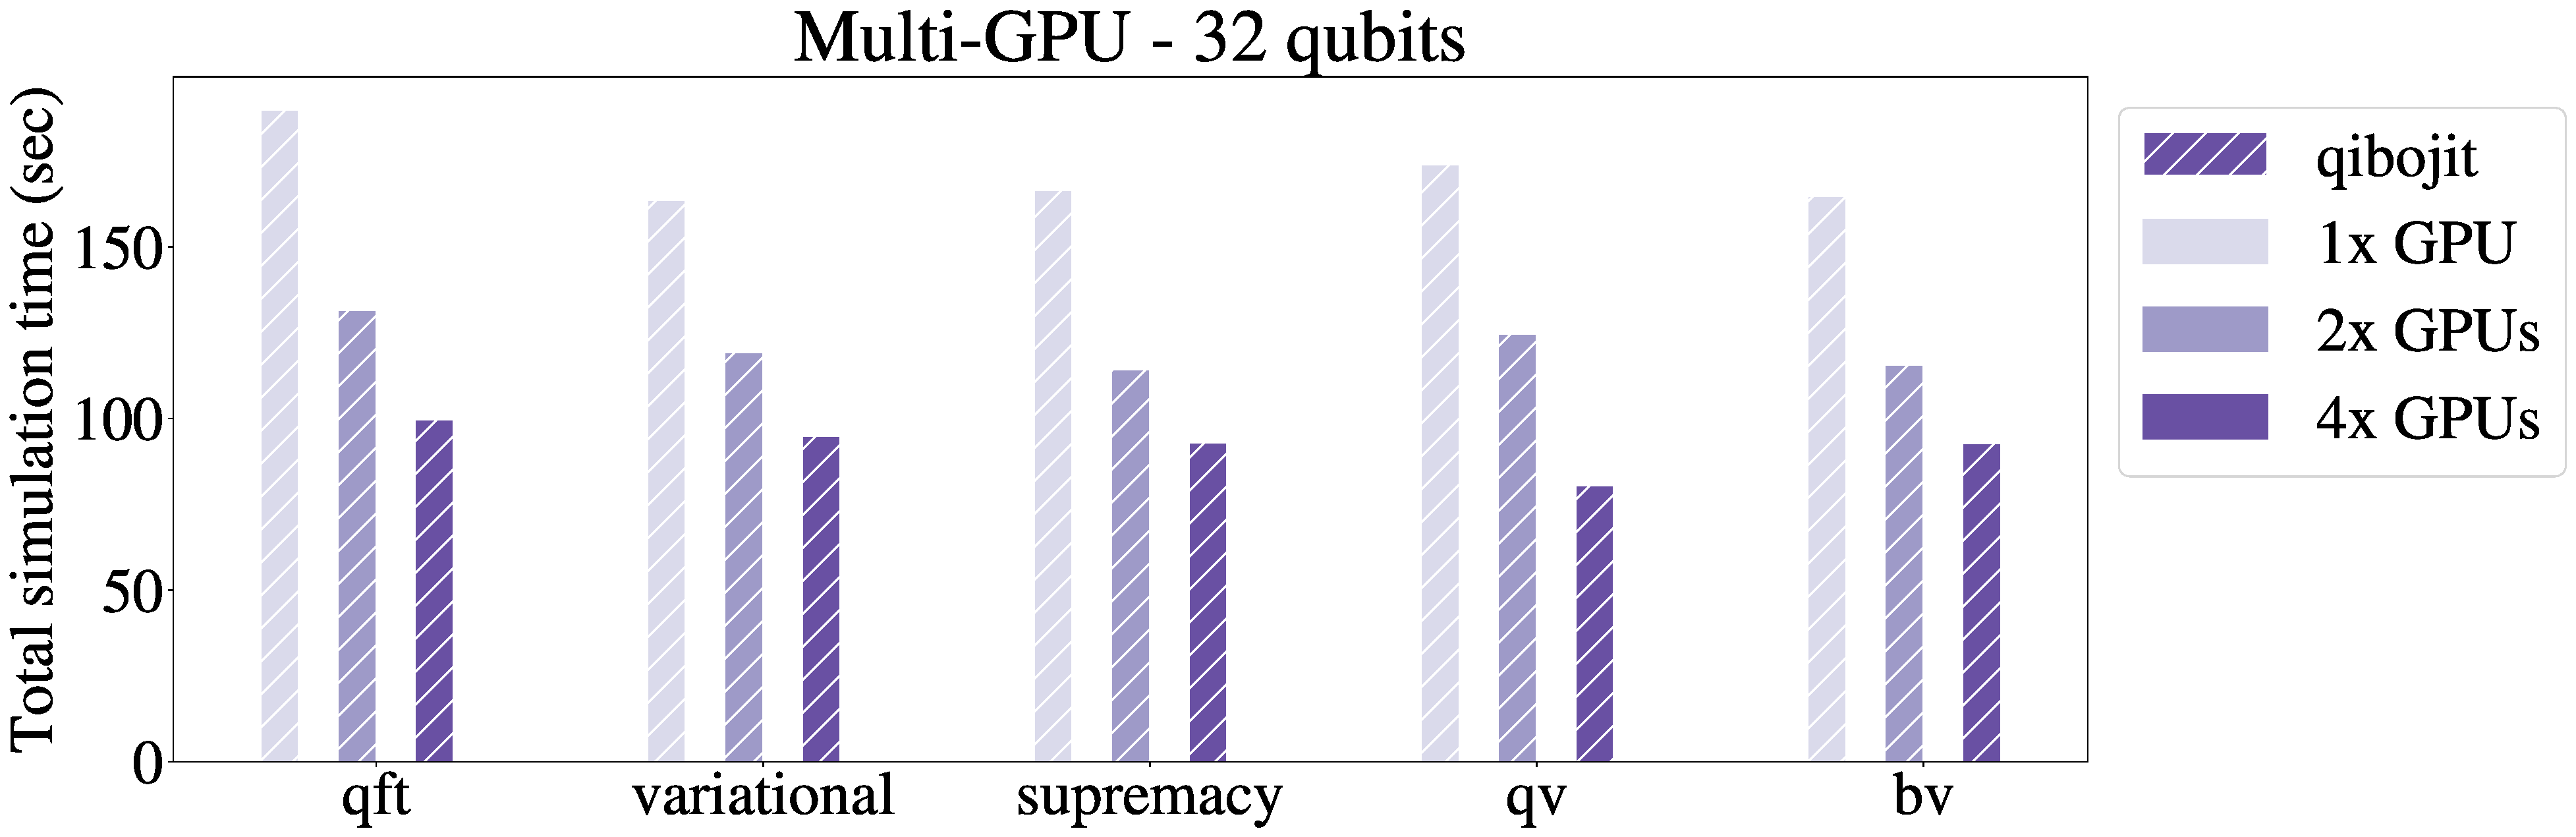
\includegraphics[width=0.8 \textwidth]{figures/multigpu_32qubits_total_simulation_time_double.pdf}
%             \end{figure}
%         \end{column}
%         \hspace{-1cm}
%         \begin{column}{0.4 \textwidth}
%             \vspace{-1cm}

%             Qibojit features
%             \begin{itemize}
%                 \item Support for CPU, GPU and multi-GPU
%                 \item NVIDIA and AMD (ROCm) GPUs
%                 \item Reduced memory footprint
%             \end{itemize}
%         \end{column}
%     \end{columns}
%     Benchmark library: \url{https://github.com/qiboteam/qibojit-benchmarks}
    
% \end{frame}


\begin{frame}{How does Qibo perform against the other libraries?}
    \begin{figure}
        \centering
        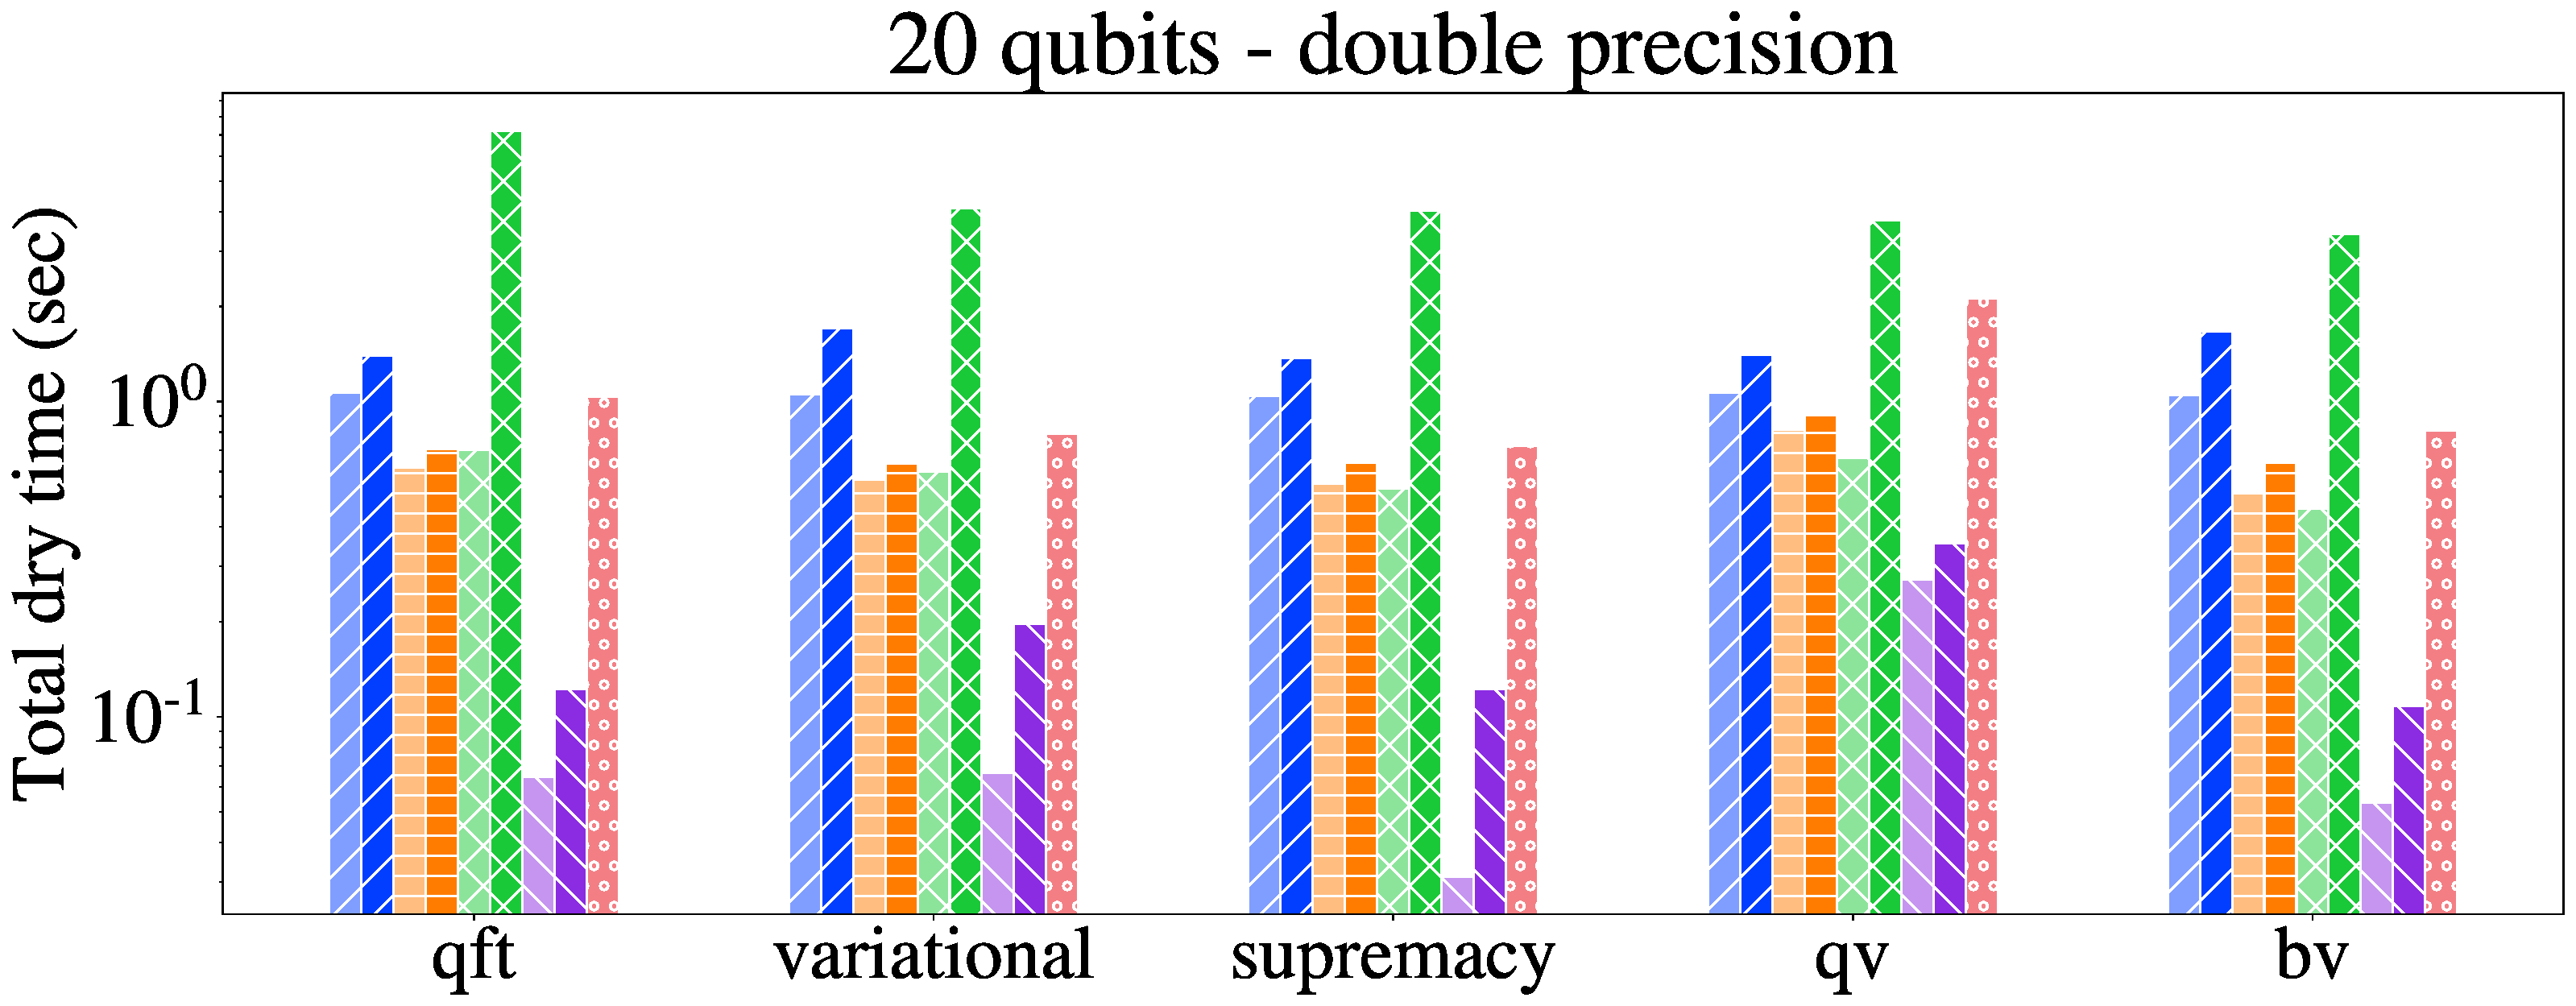
\includegraphics[height=0.4\textheight]{figures/libraries_double_20qubits_total_dry_time.pdf}
        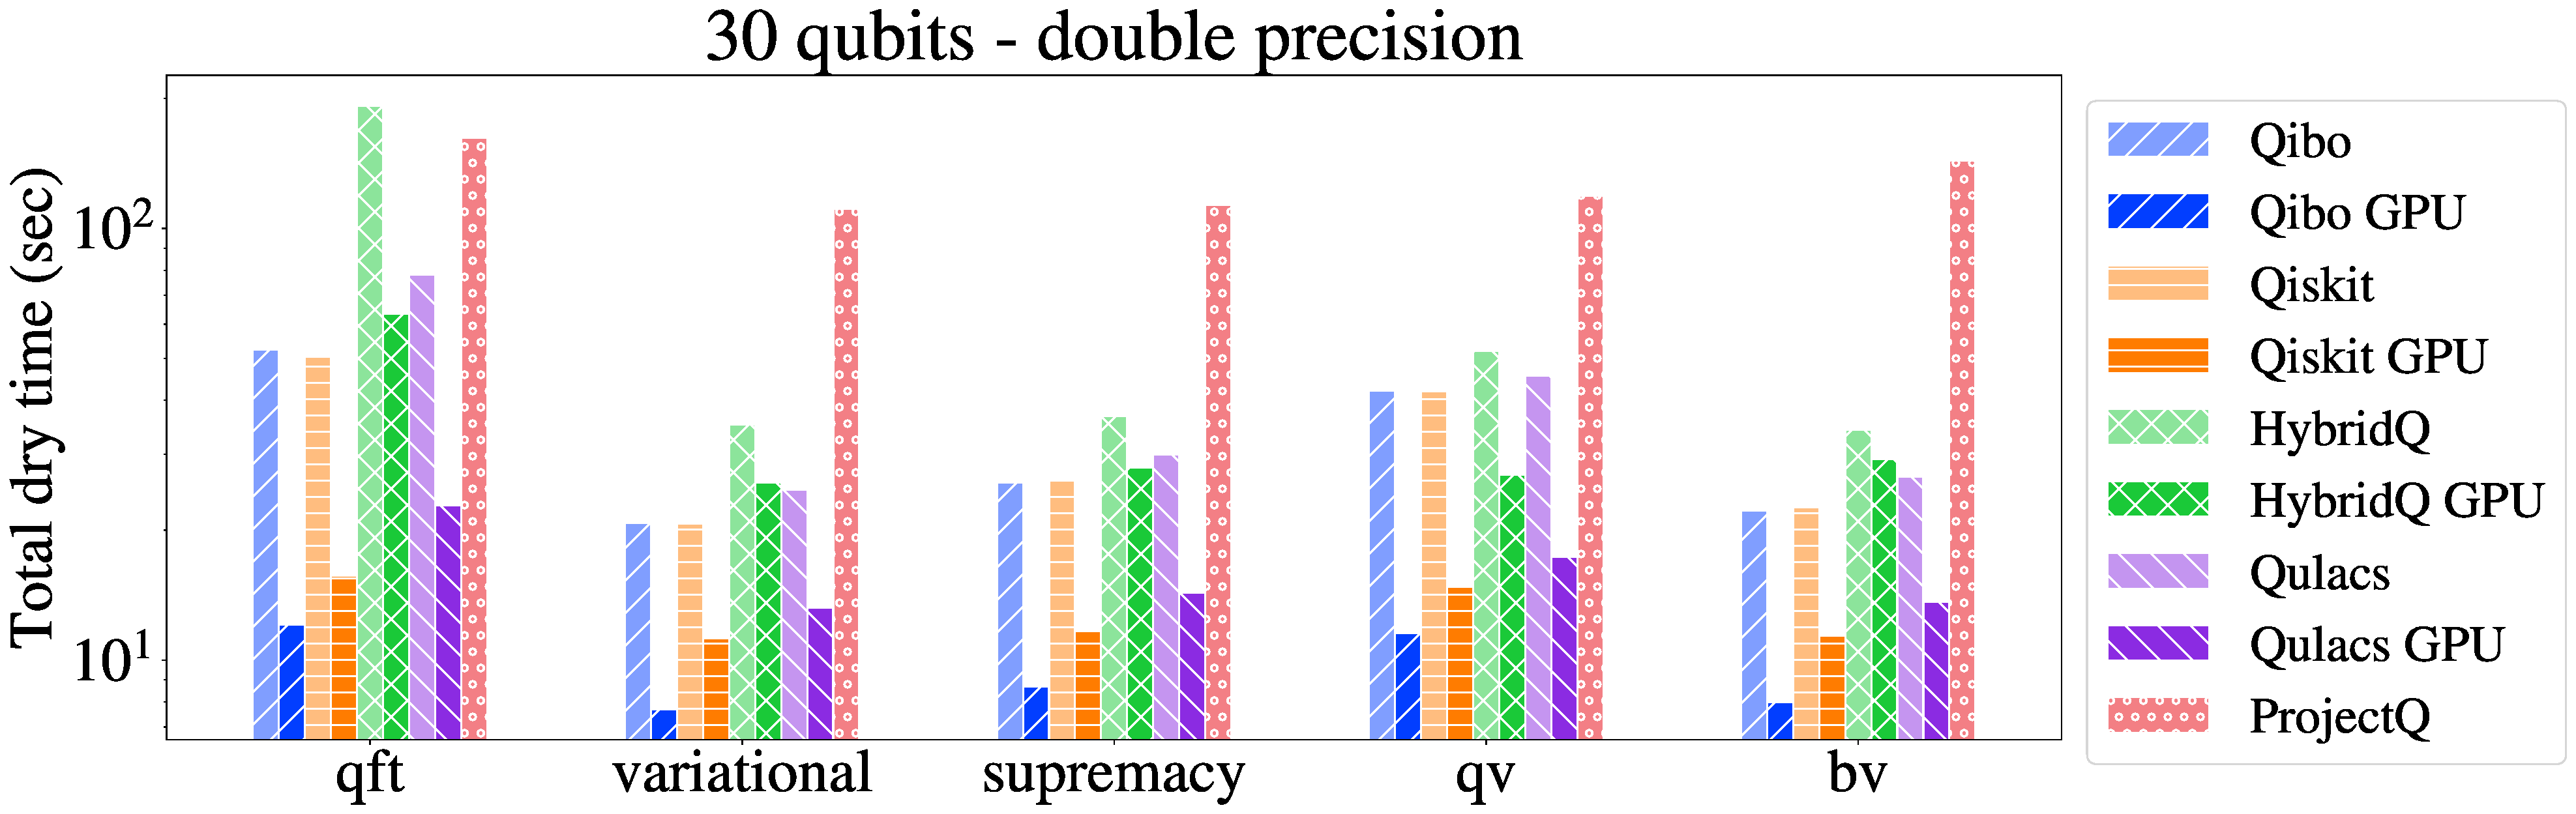
\includegraphics[height=0.31\textheight]{figures/libraries_double_30qubits_total_dry_time.pdf}
    \end{figure}
    Benchmark library: \url{https://github.com/qiboteam/qibojit-benchmarks}
    
\end{frame}

% \section{Hardware control using Qibo}

% % \begin{frame}{Hardware control}
% %     A quantum computer has many components outside the chip...
% %     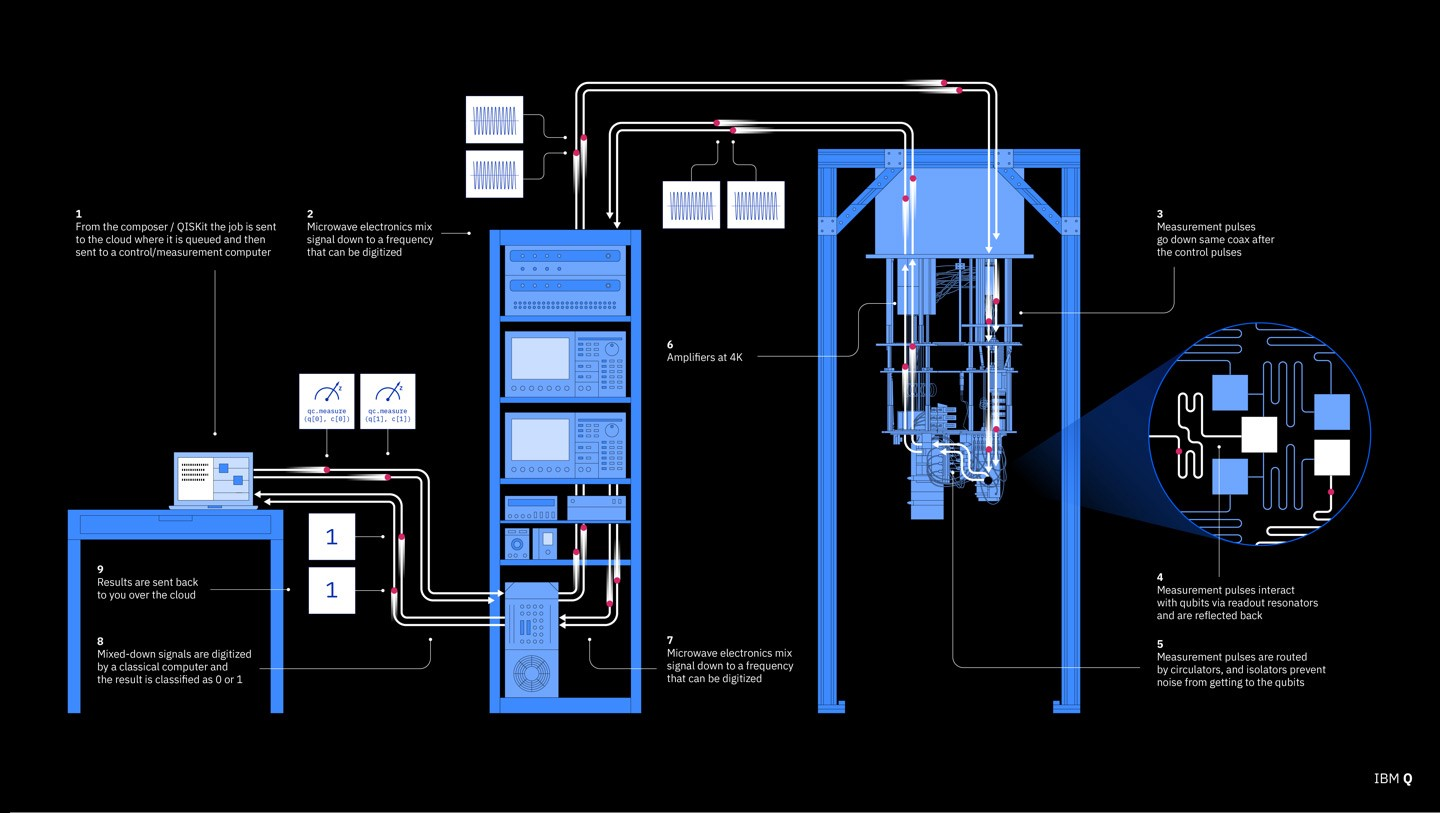
\includegraphics[width = \textwidth]{figures/quantum_computer.jpeg}


    
% % \end{frame}

% \begin{frame}{Hardware control}
%     For superconducting qubits \textbf{gates} are implemented by sending \textbf{pulses}.

%     \begin{columns}
%         \begin{column}{0.5 \textwidth}
%             \begin{figure}
%                 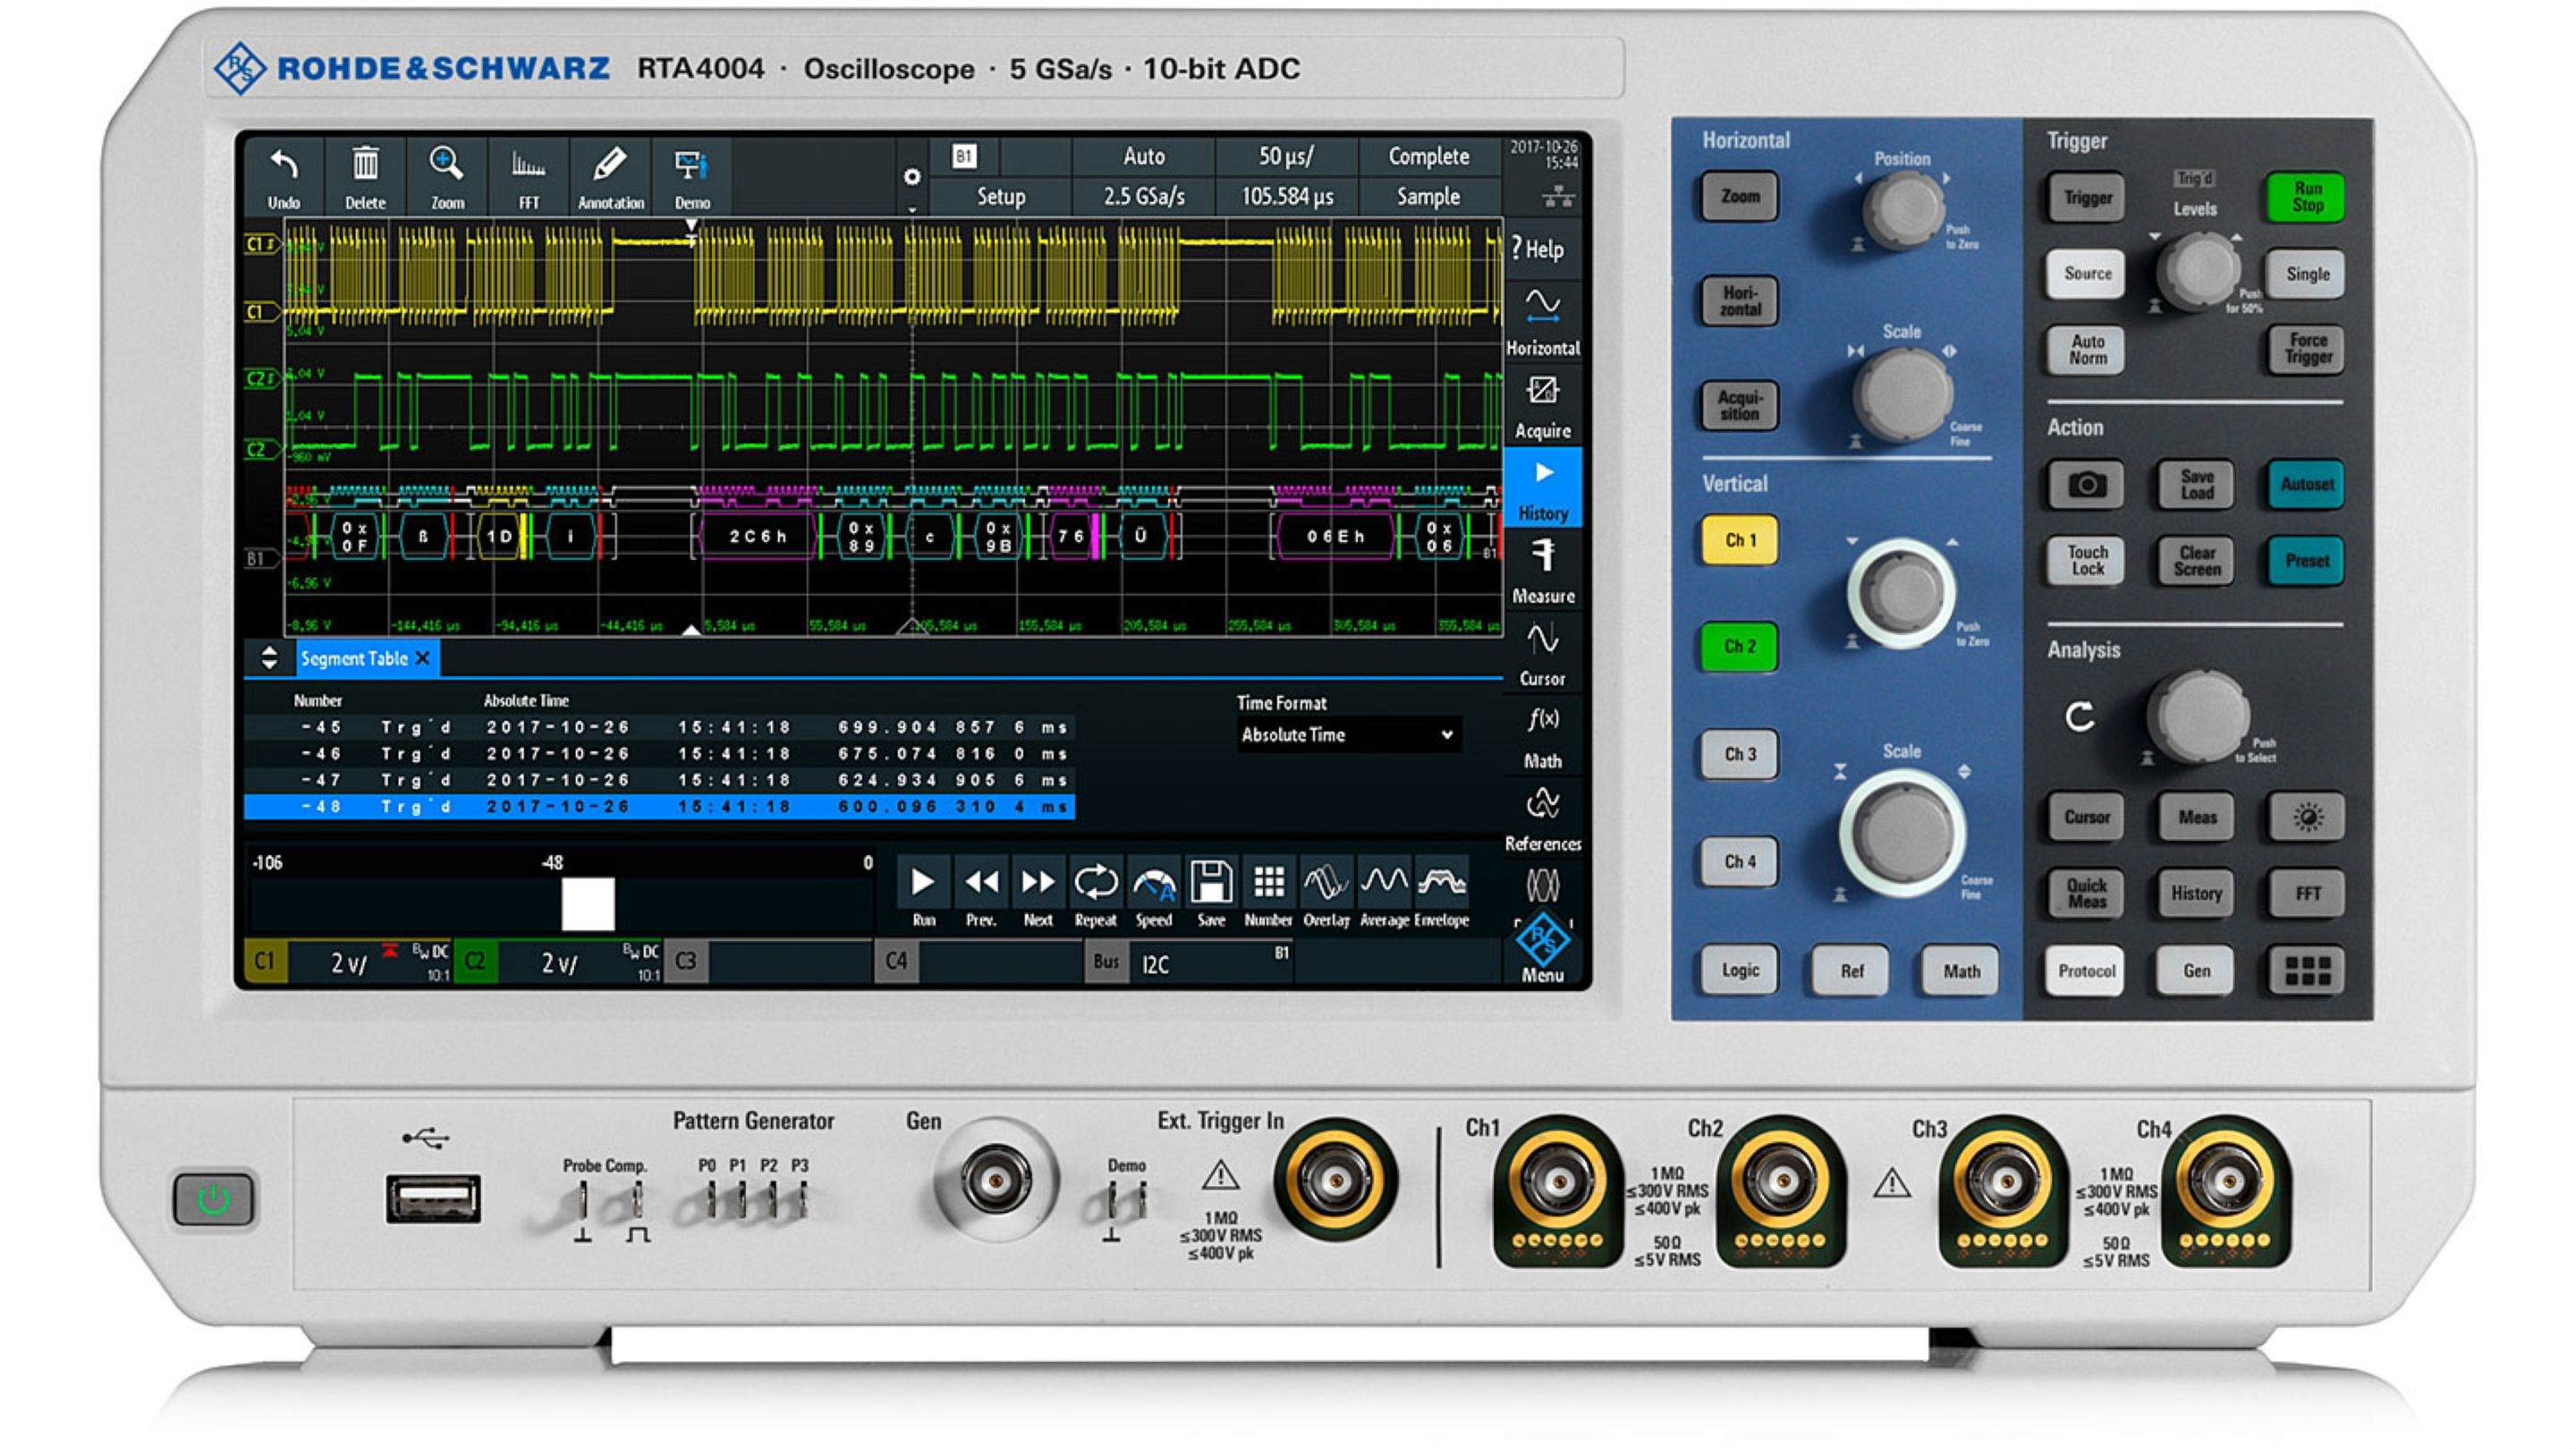
\includegraphics[height = 0.3 \textheight]{figures/rohde.jpg}
%                 % \caption{Oscilloscope}
%             \end{figure}
            
%             % \begin{itemize}
%             %     \item Wavefunction generators
%             %     \item Local oscillators
%             %     \item Qblox devices
%             %     \item Custom FPGA boards
%             %    \end{itemize}
%         \end{column}
%         \begin{column}{0.5 \textwidth}
%             % 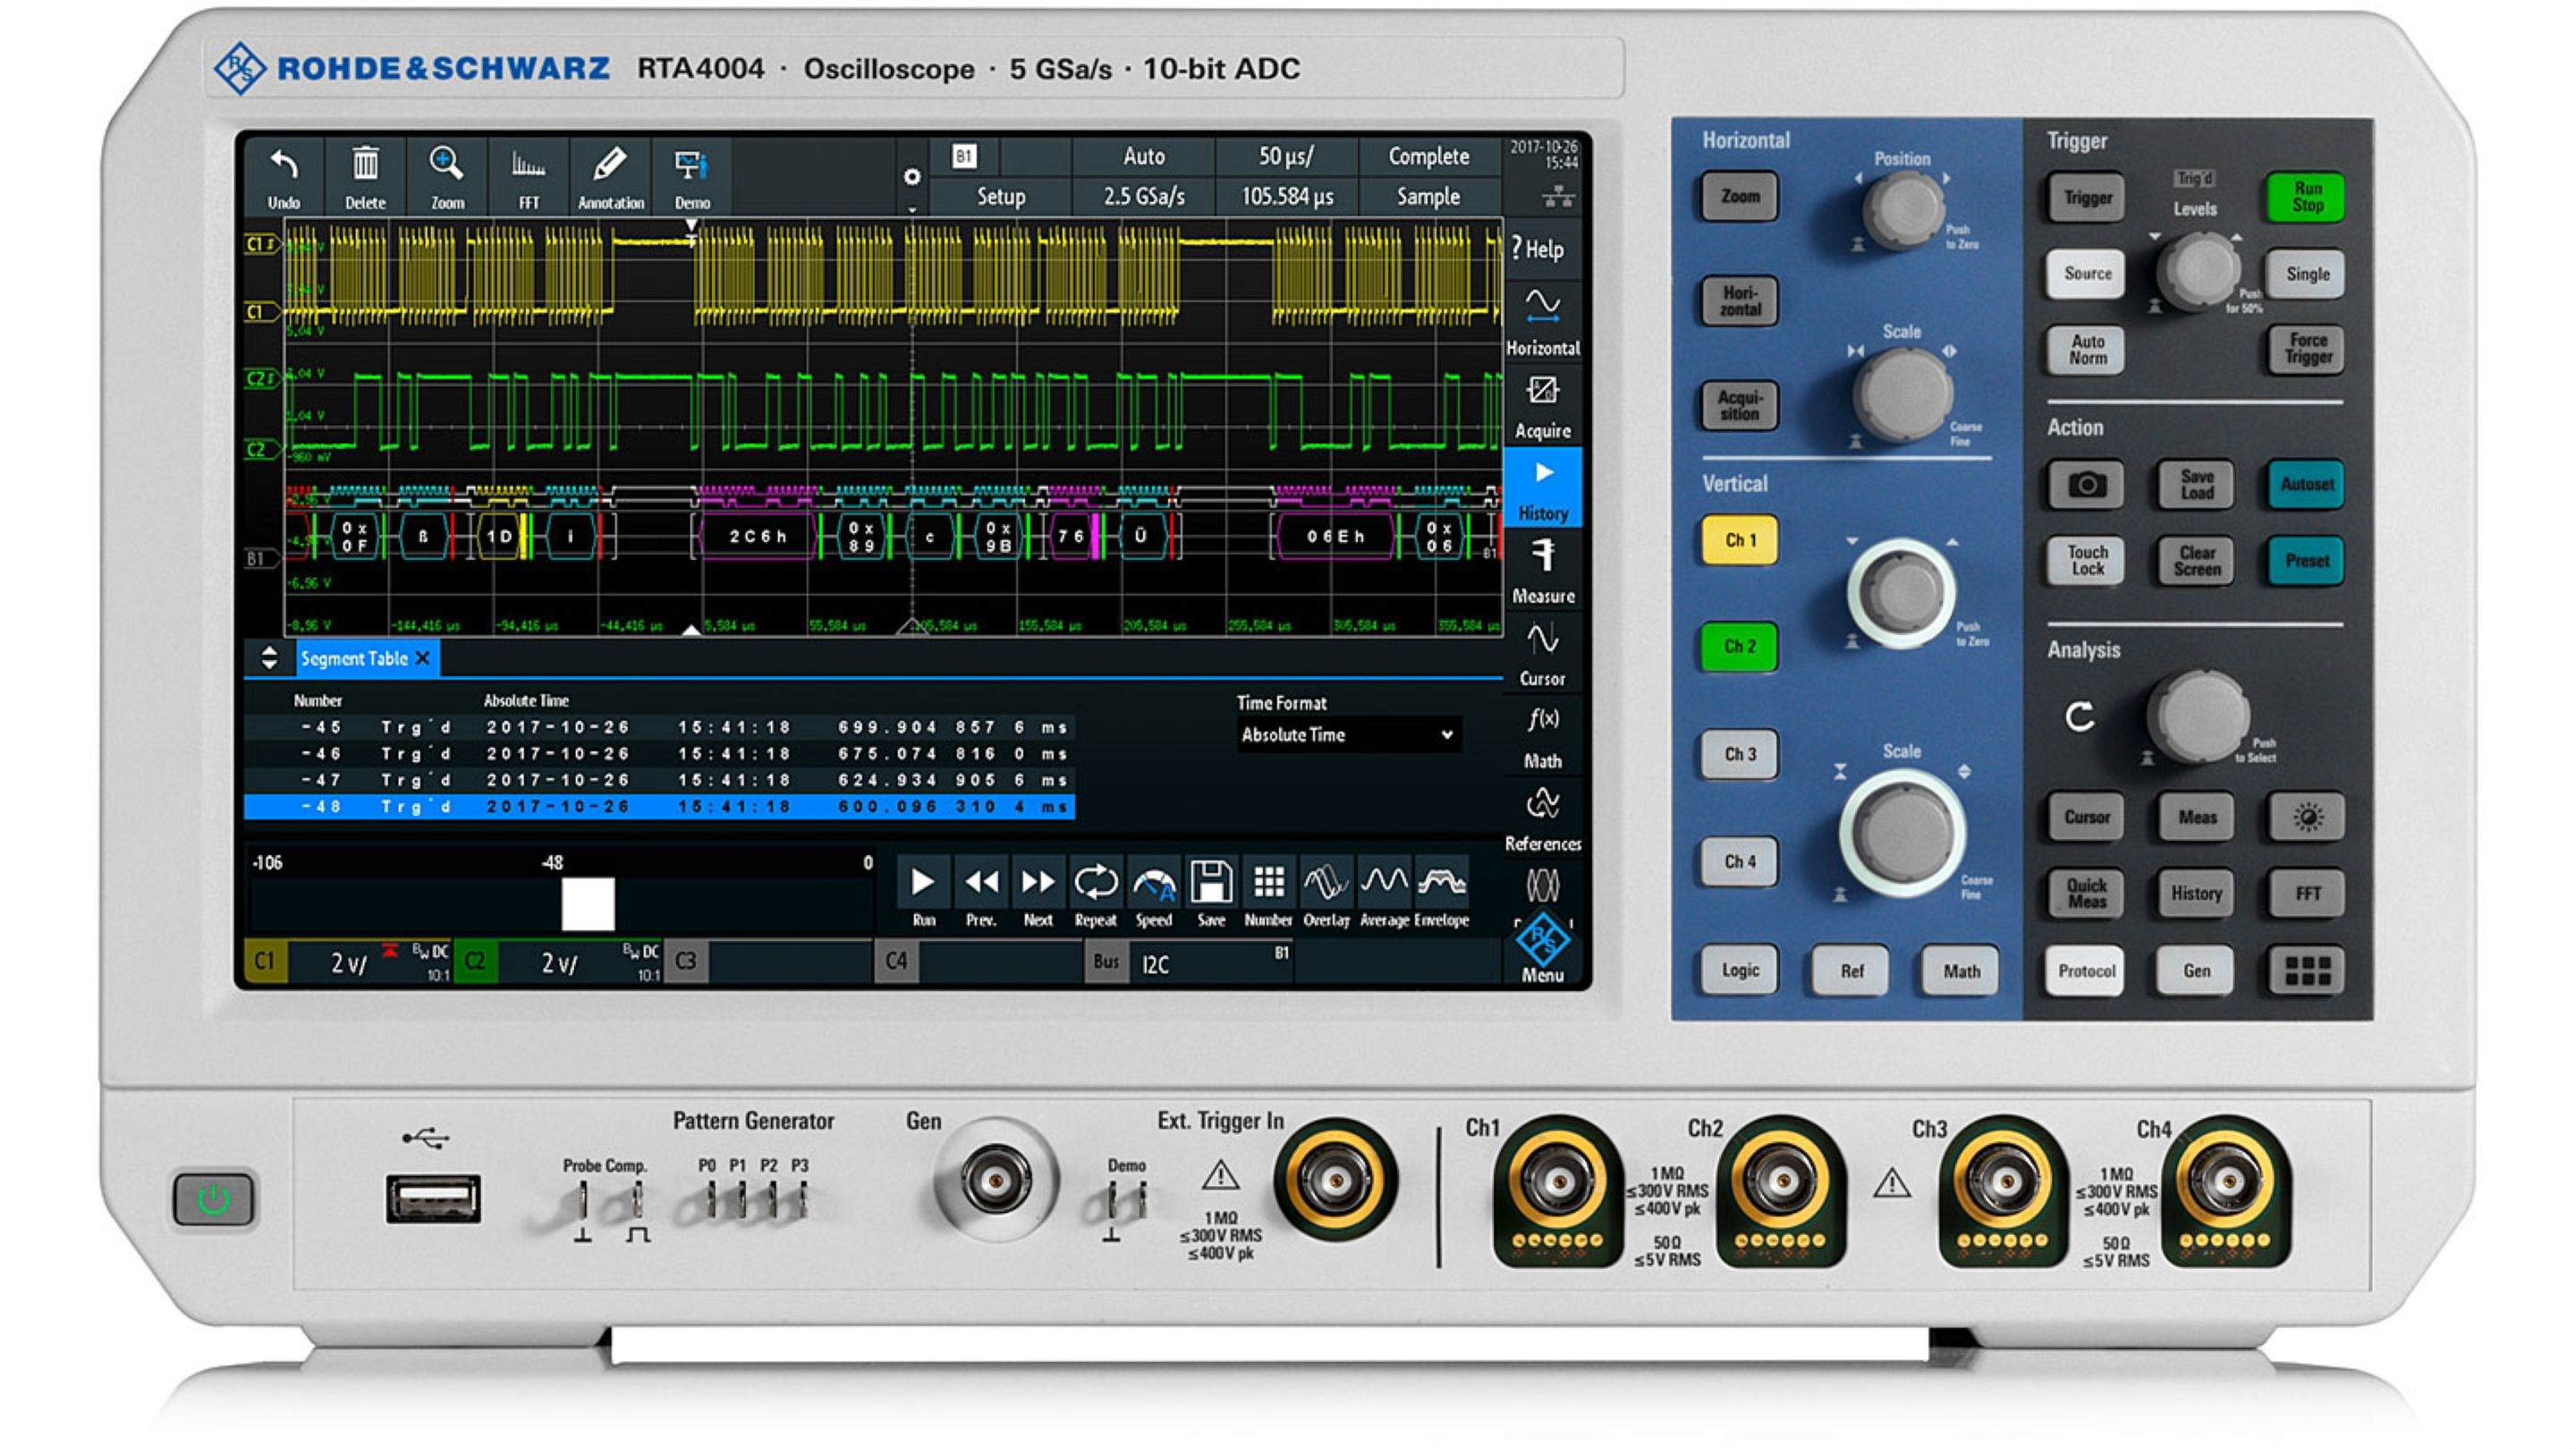
\includegraphics[height = 0.3 \textheight]{figures/rohde.jpg}
%             \begin{figure}
%                 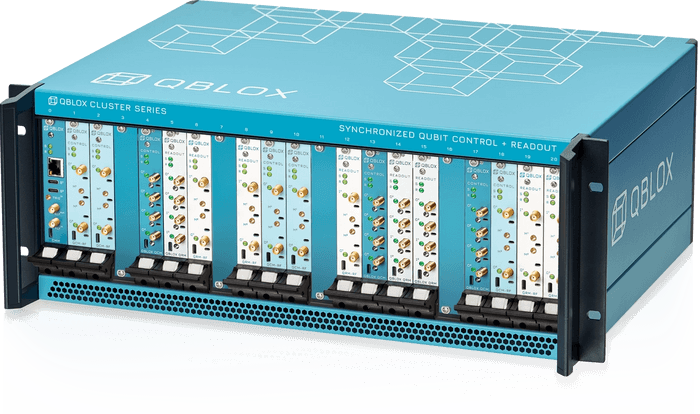
\includegraphics[height = 0.3 \textheight]{figures/qblox.png}
%                 % \caption{Qblox}
%                 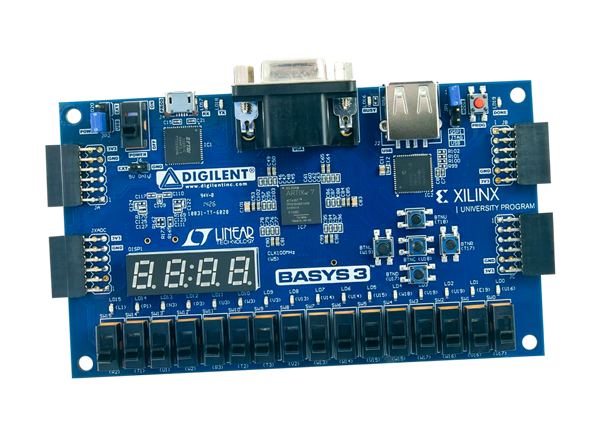
\includegraphics[height = 0.3 \textheight]{figures/fpga.png}
%                 % \caption{FPGA board}
%             \end{figure}
            
%         \end{column}
%     \end{columns}
  
%    We need a framework to control all these devices at the same time.
    
% \end{frame}

% \begin{frame}{Introducing Qibolab}
%     \begin{columns}
%         \begin{column}[]{0.5 \textwidth}
%             \begin{figure}
%                 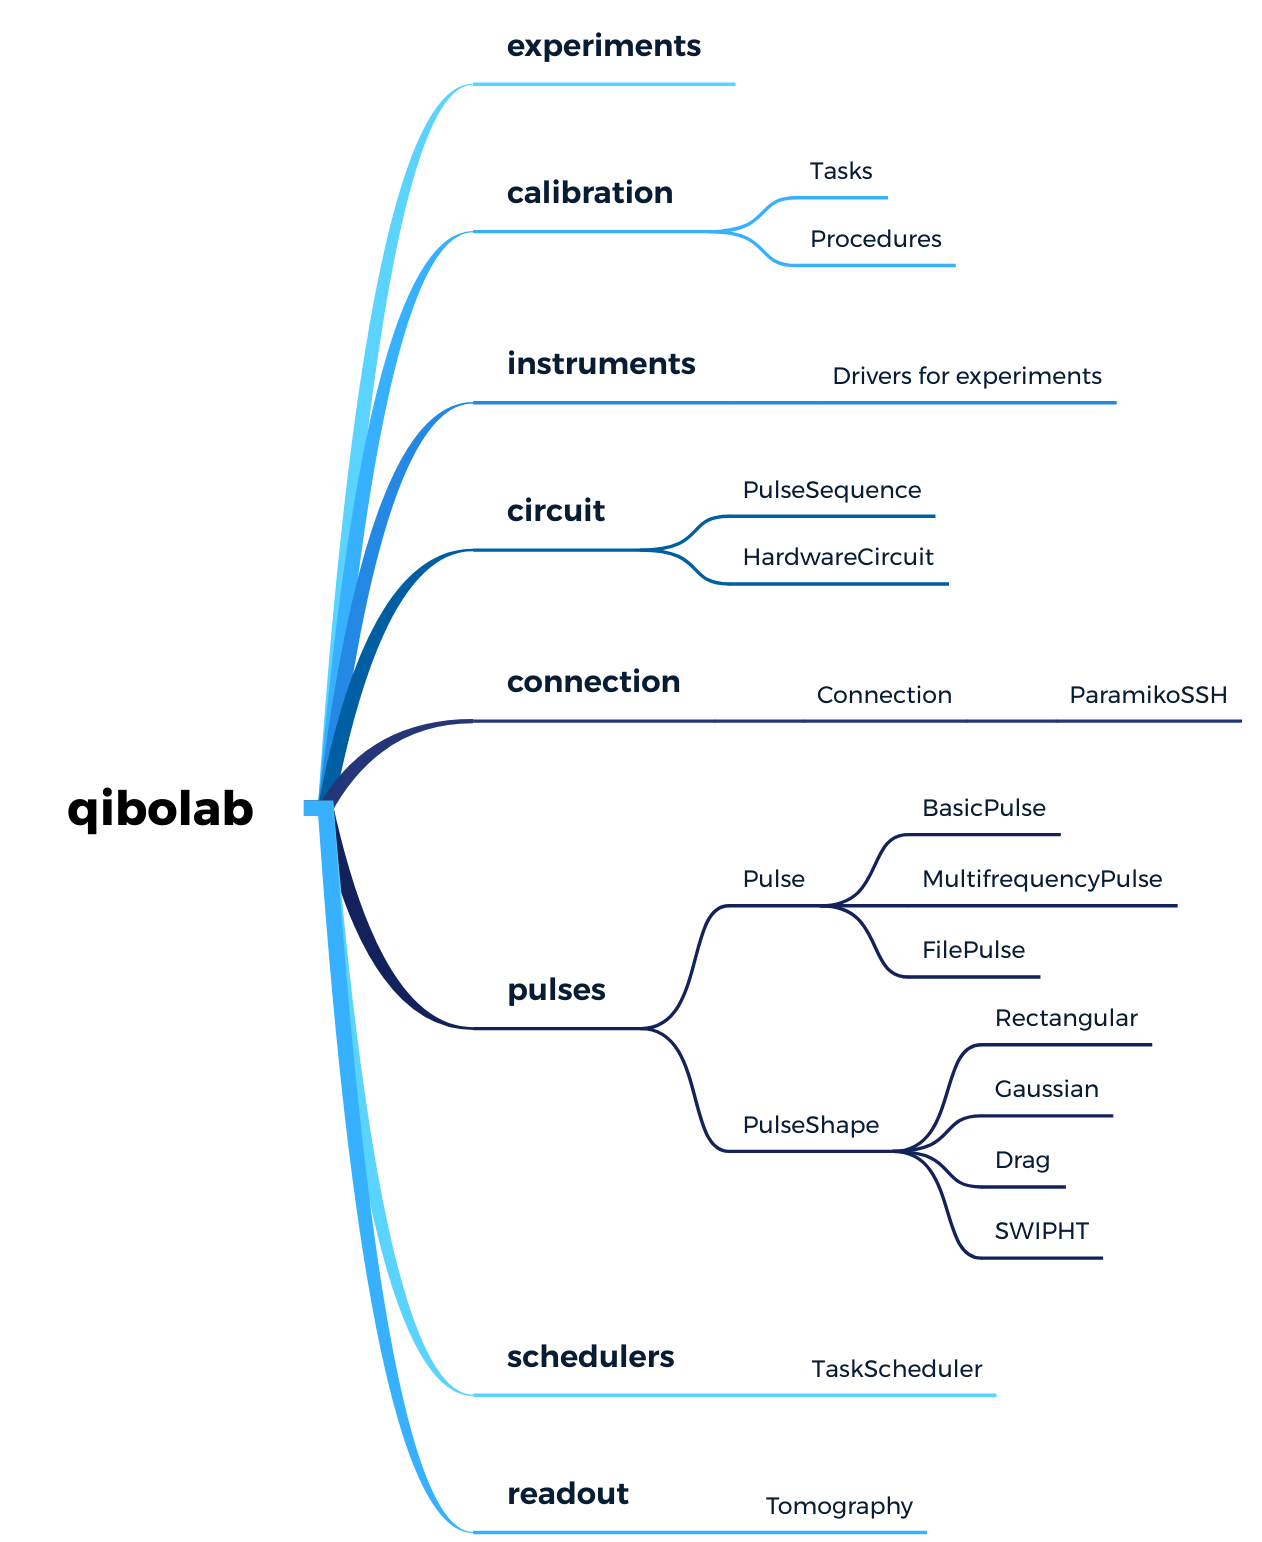
\includegraphics[height=0.8\textheight]{figures/qibolab.png}
%             \end{figure}
            
%         \end{column}

%         \begin{column}[]{0.5 \textwidth}
%             \begin{tcolorbox}[colframe=gray,title=Qibolab features:]
%                 \begin{itemize}
%                     \item Deploy Qibo models on quantum hardware easily
%                     \item User-friendly Pulse API
%                     \item Create custom experimental drivers for lab setup
%                     \item Support multiple heterogeneous platforms
%                 \end{itemize}
%                 \end{tcolorbox}
%         \end{column}
%     \end{columns}
% \end{frame}

% \begin{frame}{How to use qibolab?}
%     \begin{figure}
%         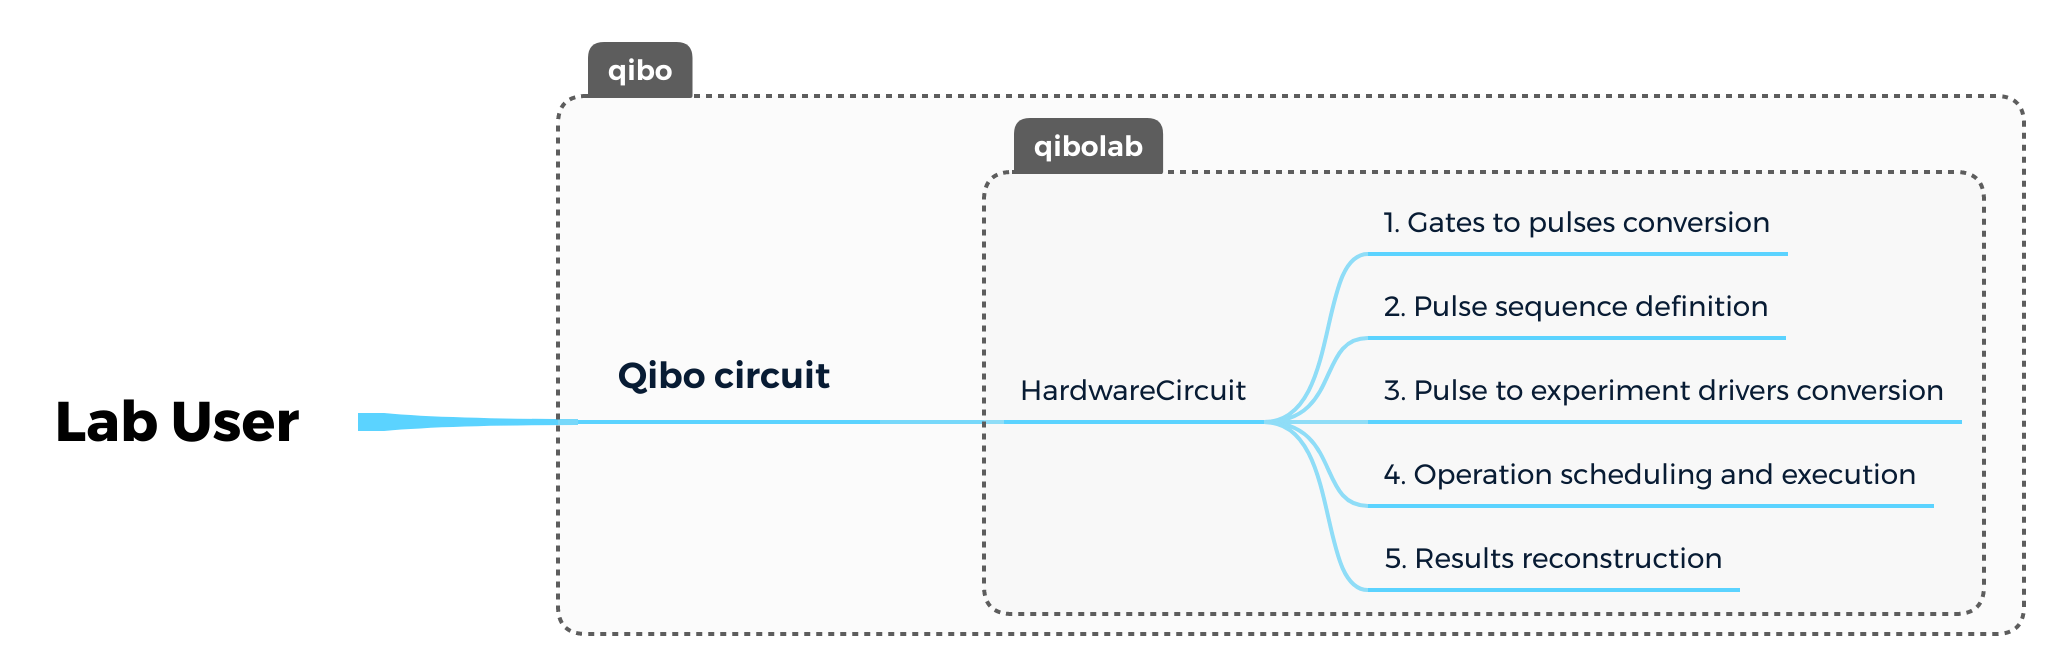
\includegraphics[width=\textwidth]{figures/hardwarecircuit.png}
%     \end{figure}

%     \begin{columns}
%         \begin{column}{0.5 \textwidth}
%             \begin{figure}
%                 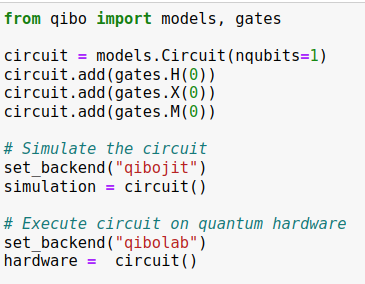
\includegraphics[width = \columnwidth]{figures/qibo__circuit.png}
%             \end{figure}
%         \end{column}
%         \begin{column}{0.5 \textwidth}
%             \begin{itemize}
%                 \item A single object to execute both on hardware and simulation
%                 \item Job scheduling to access the hardware using slurm
%             \end{itemize}
%             \centering
%             
\includegraphics[height=2cm]{figures/Slurm_logo.svg.png}
%         \end{column}
%     \end{columns}

% \end{frame}

% \begin{frame}{Quantum Machine Learning on Real Hardware}
% 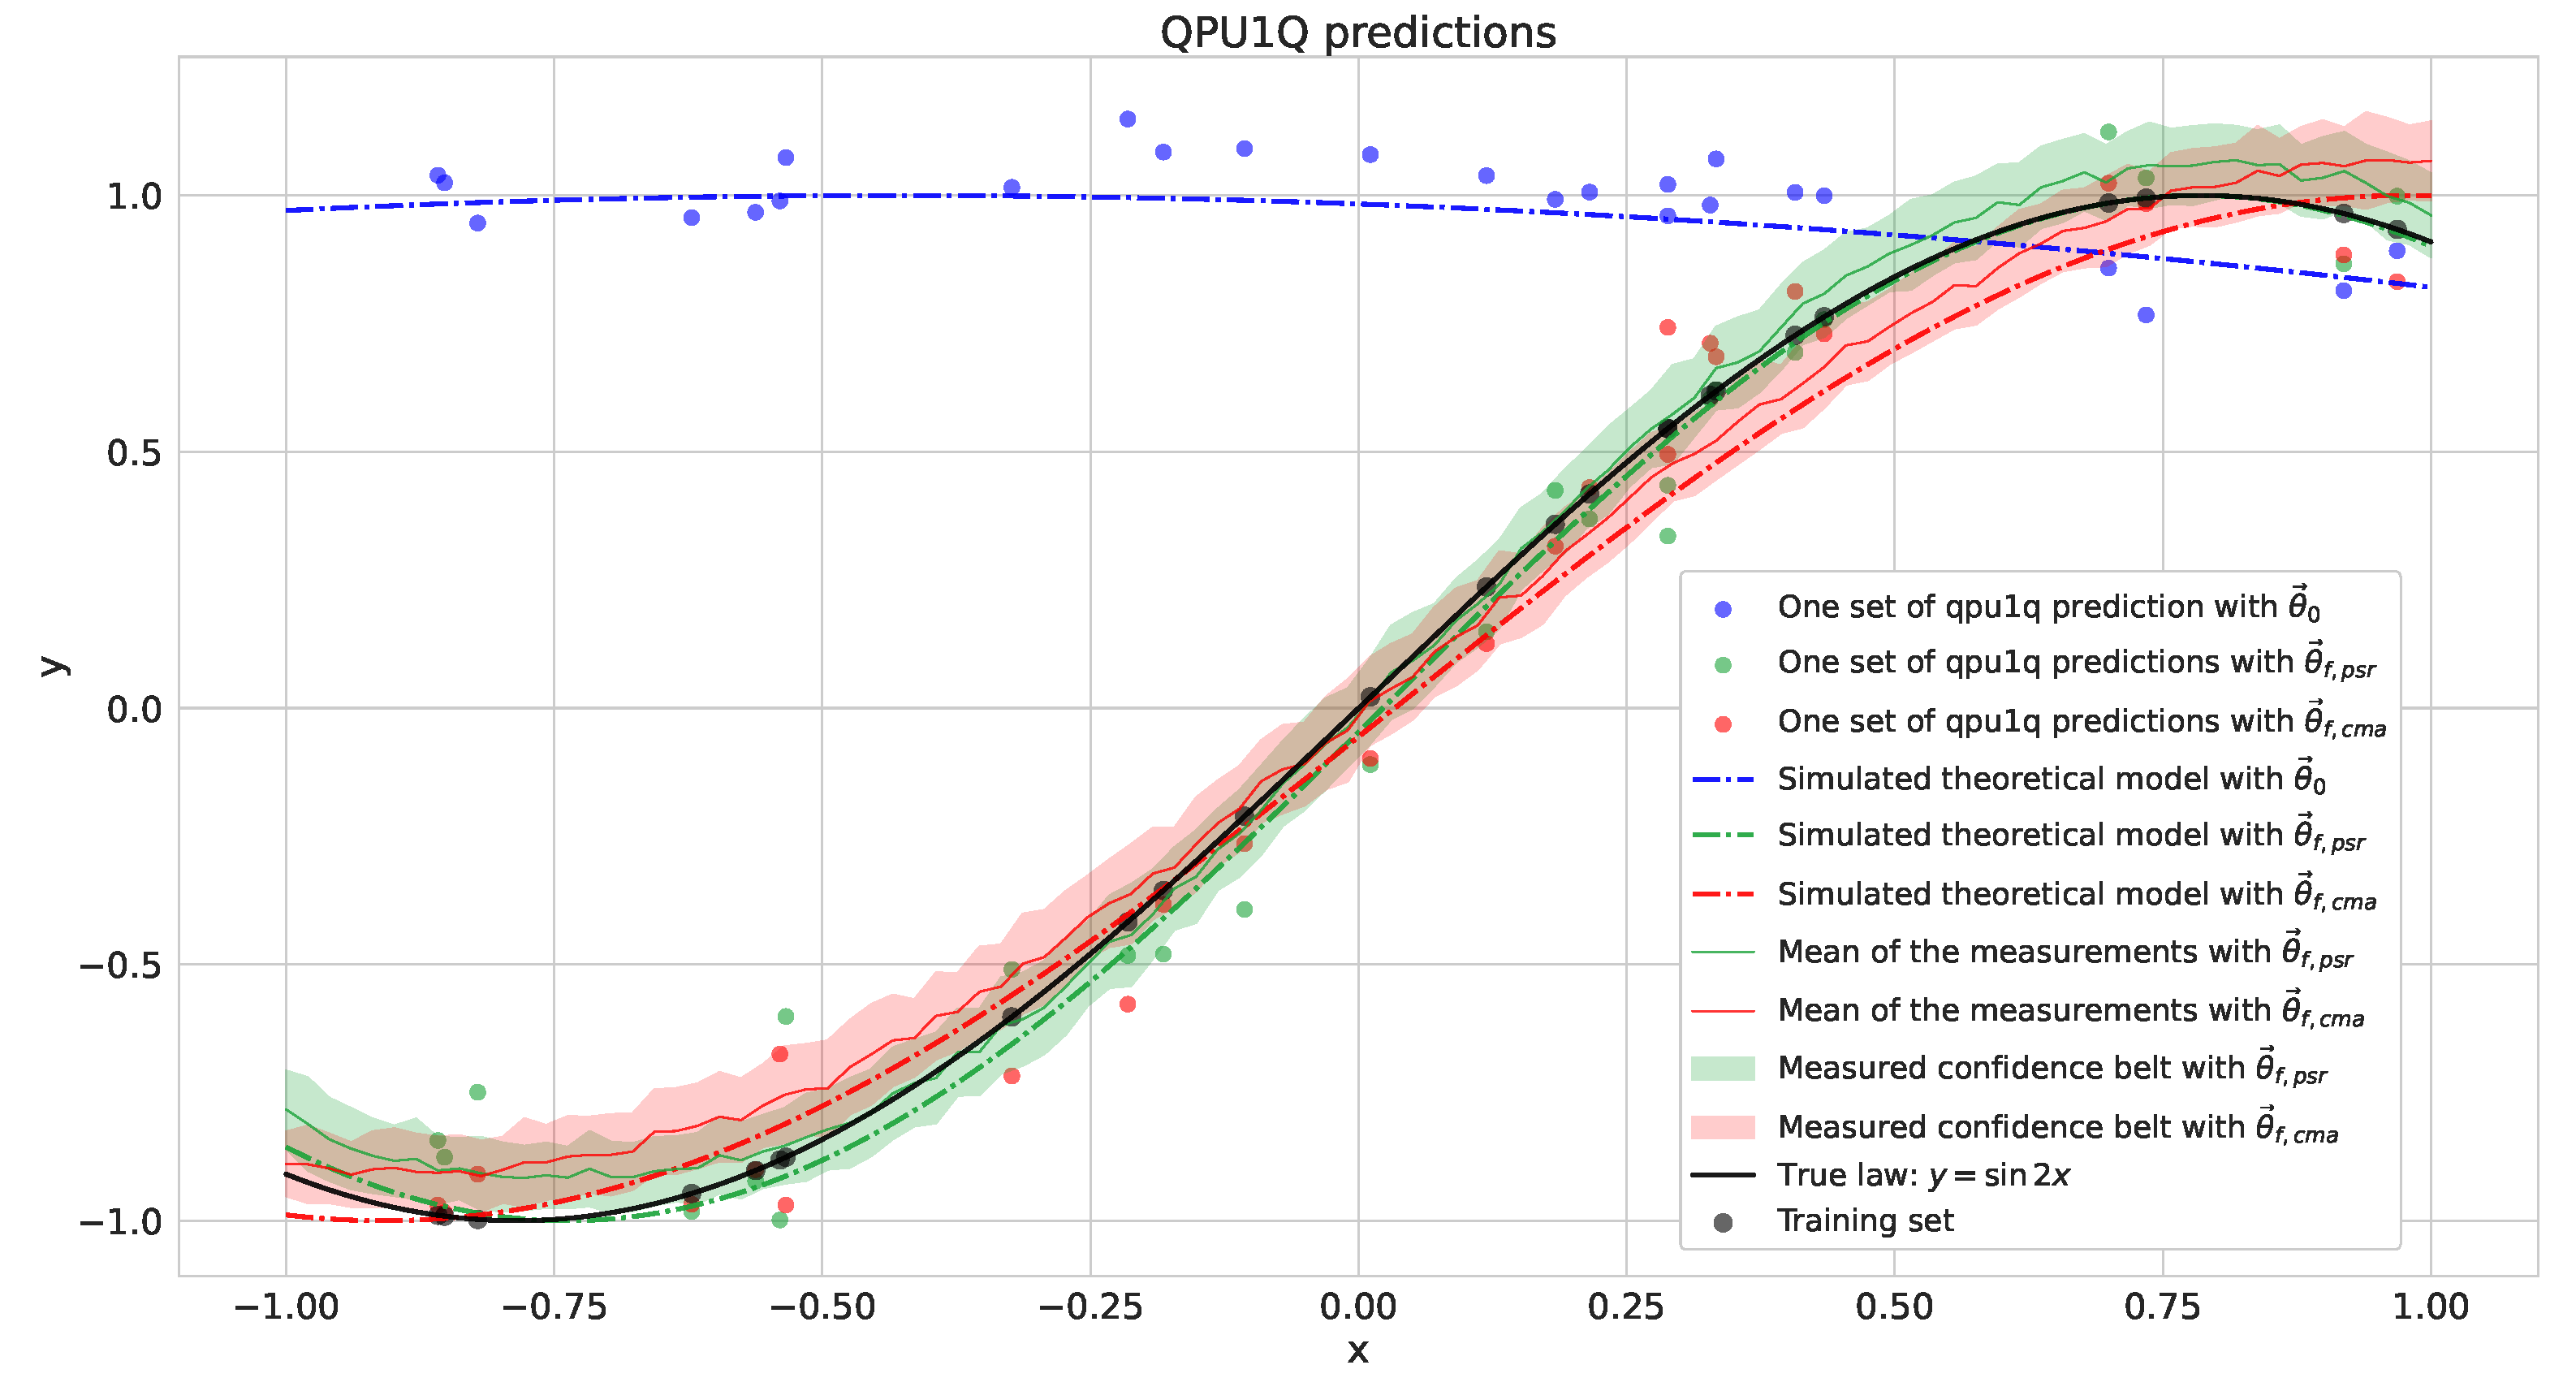
\includegraphics[width=\textwidth]{figures/cropped_qpu_not_normed..pdf}
% \end{frame}



% \section{A reporting tool for calibration using Qibo}

% \begin{frame}{Difficulties}
%     Suppose that we have assembled a quantum computer and we have a way
%     to send pulses to the chip... are we done? {\color{red} \textbf{No} }

%     We need to { \color{blue} characterize}, { \color{blue} validate} and { \color{blue} verificate} our qubits (QCVV):
%     \begin{columns}
%         \begin{column}{0.5 \textwidth}
%             \vspace{-2cm}
%             \begin{itemize}
%                 \item[\faCaretSquareORight] Perform standard calibration routines:
%                 \begin{itemize}
%                     \item[\faWrench] Resonator and qubit spectroscopy
%                     \item[\faWrench] Rabi and Ramsey 
%                     \item[\faWrench] T1 and T2 determination
                
%                 \end{itemize}
%                 \item[\faCaretSquareORight] Perform quantum protocols to extract the fidelity:
%                 \begin{itemize}
%                     \item[\faWrench] Randomized Benchmarking
%                     \item[\faWrench] Gate Set Tomography
%                     \item[\faWrench] Cross-Entropy Benchmarking
%                 \end{itemize}
%                 \item[\faCaretSquareORight] Repeat the above steps periodically.
%             \end{itemize}
%         \end{column}
%         \begin{column}{0.5 \textwidth}
%             \begin{figure}
%                 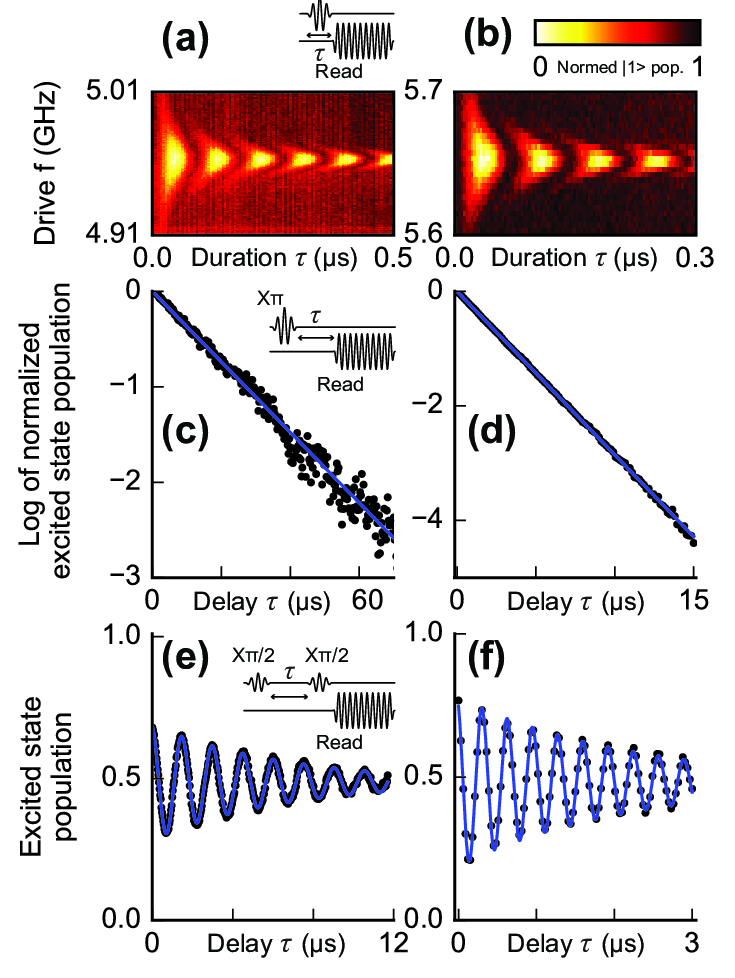
\includegraphics[width = 0.8 \textwidth]{figures/characterization.png}
%             \end{figure}
            
%         \end{column}
%     \end{columns}
    

% \end{frame}

% \begin{frame}{A new reporting tool for Qibo}
%     We are developing a new tool that it will be able to perform QCVV in Qibo
%     with the following features:
%             \begin{multicols*}{2}
%                 \begin{itemize}
%                     \item[\faCaretSquareORight] Platform agnostic
%                     \item[\faCaretSquareORight] Launch calibration routine easily
%                     \item[\faCaretSquareORight] Live-plotting tools
%                     \item[\faCaretSquareORight] Live-fitting tools
%                     \item[\faCaretSquareORight]Save and share your data
%                     \item[\faCaretSquareORight] Autocalibration routines
%                 \end{itemize}
%             \end{multicols*}
%             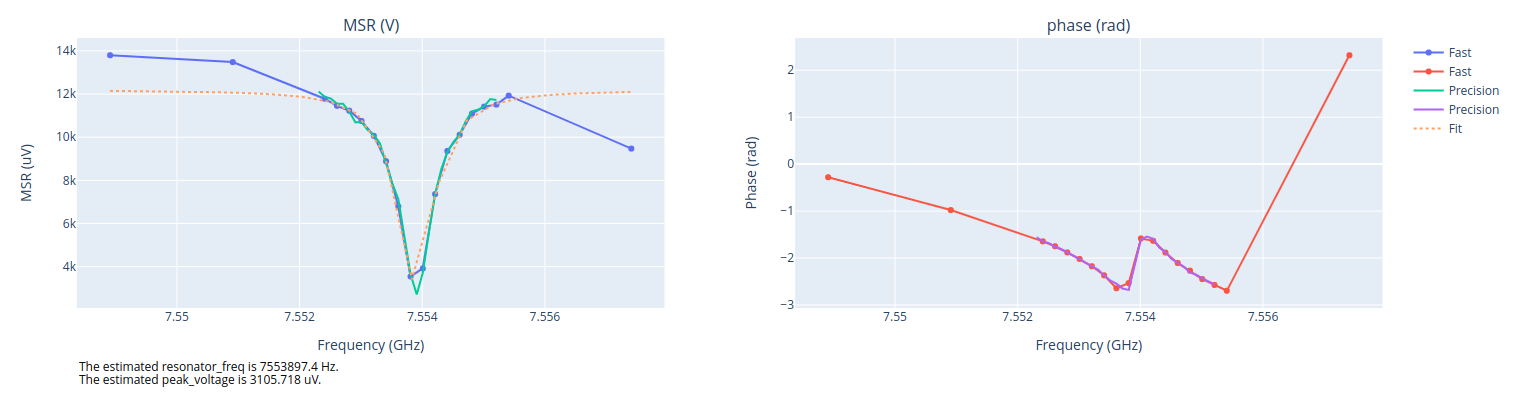
\includegraphics[width=\textwidth]{figures/resonator.png}
            

   
% \end{frame}

% \begin{frame}{Report example}
    
%     \begin{figure}
%         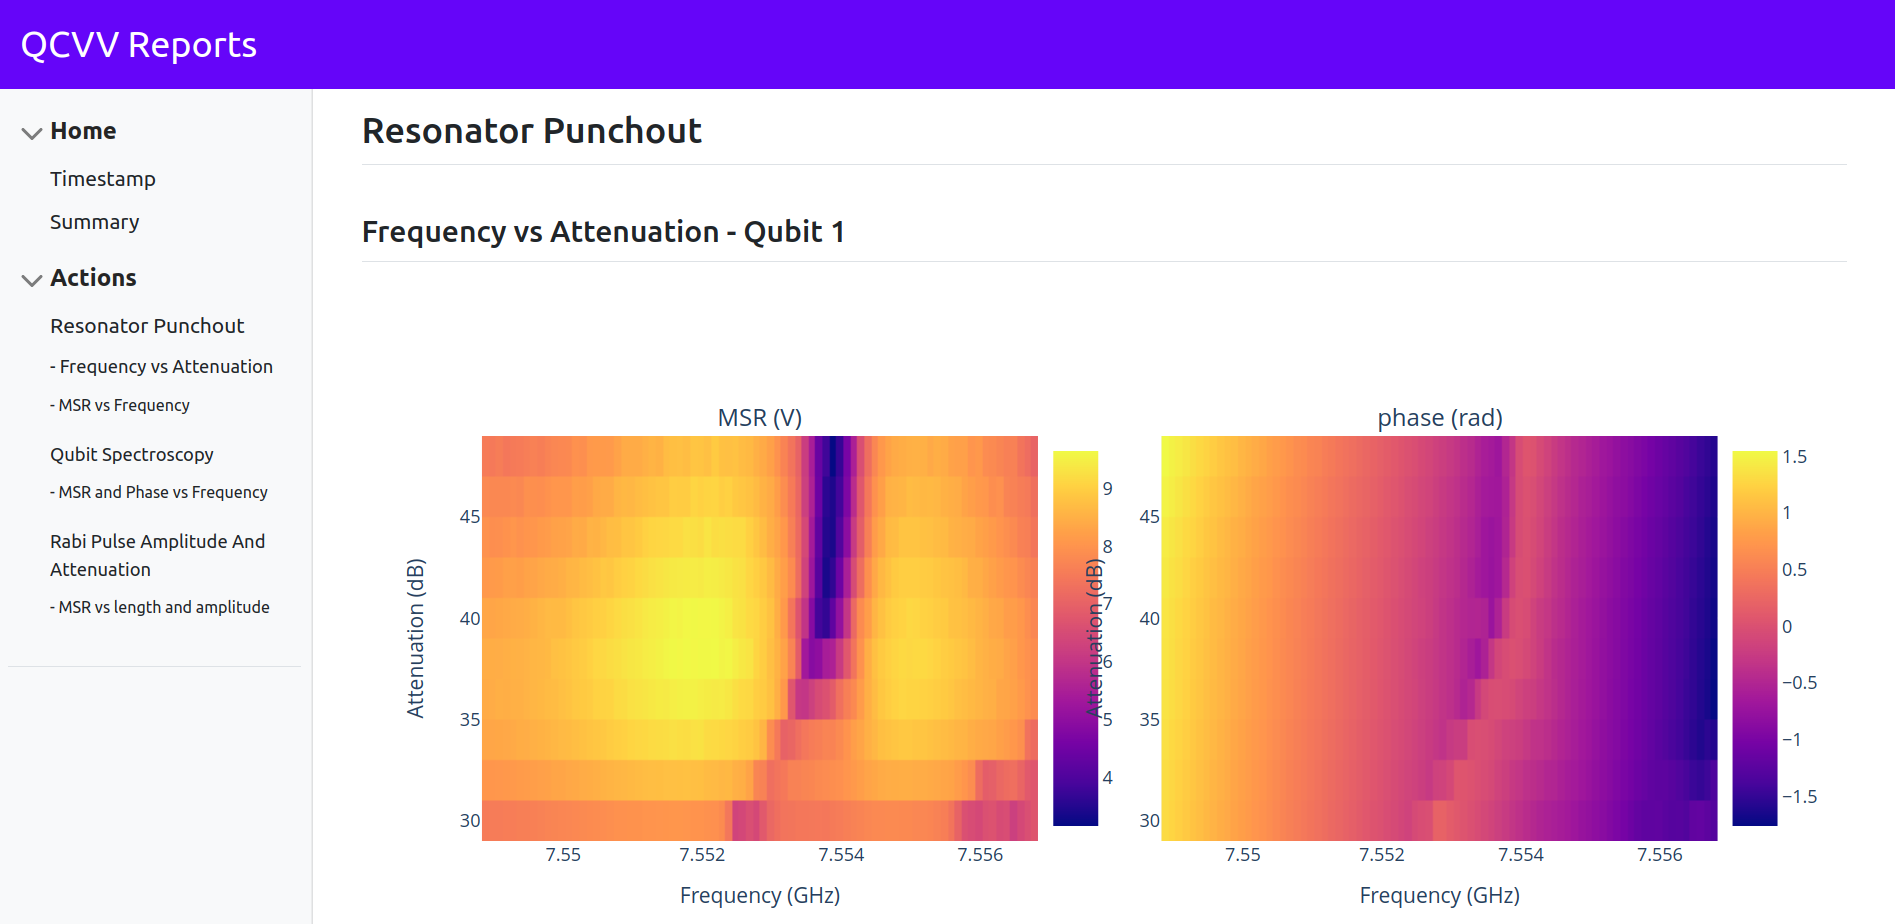
\includegraphics[width=\textwidth]{figures/qcvv.png}
%         % 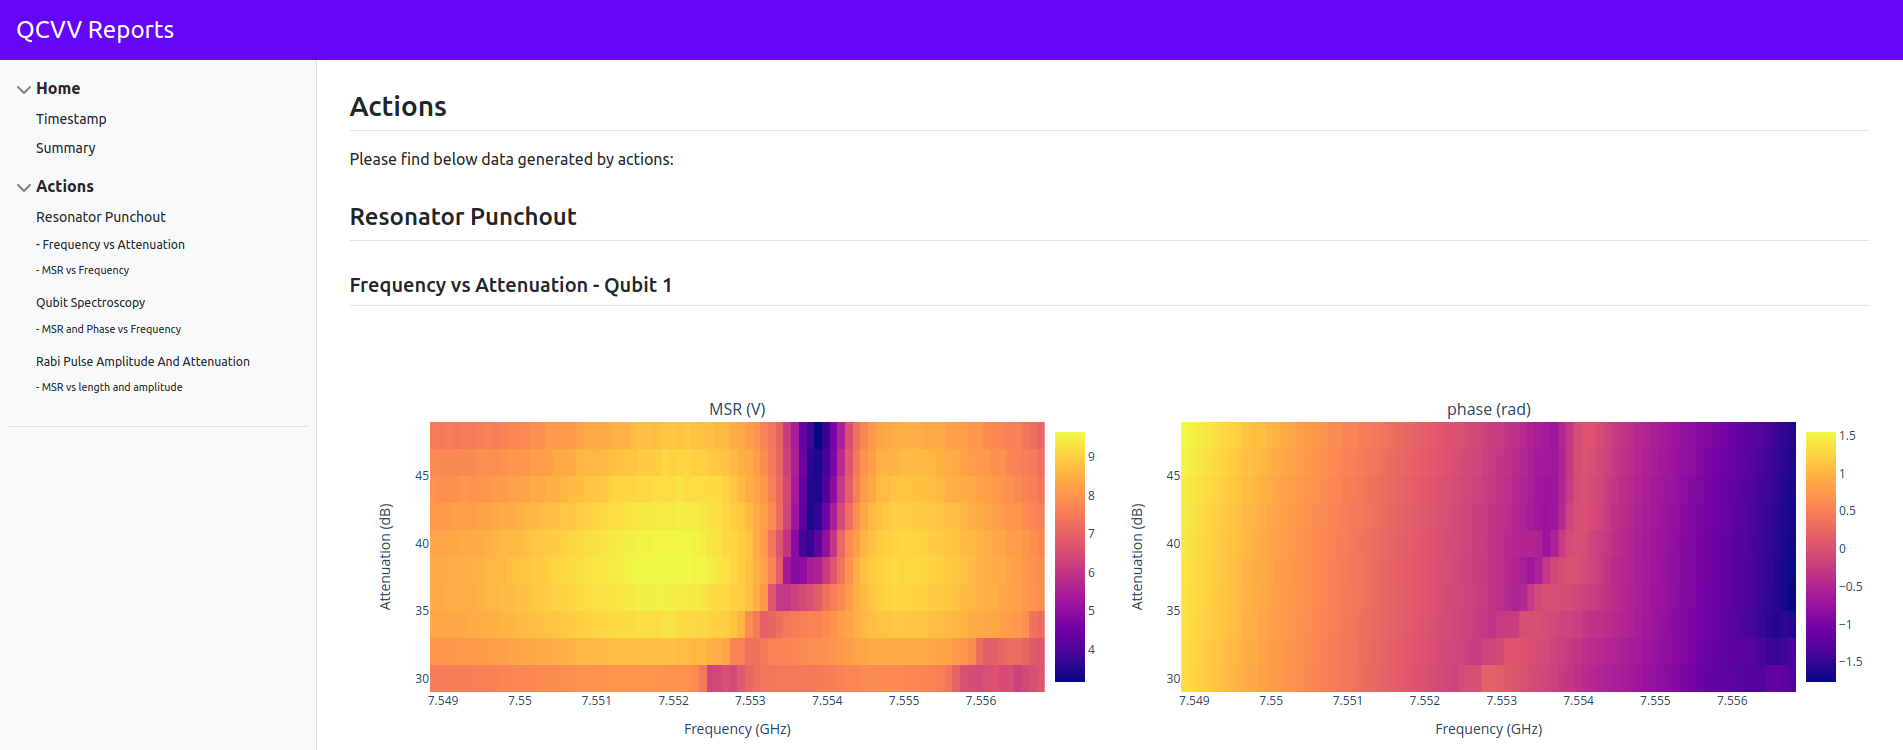
\includegraphics[width=\textwidth]{figures/punchout.png}
%     \end{figure}
    
% \end{frame}

\section{Grover's algorithm}

\begin{frame}{What is Grover’s Algorithm?}
    Grover’s algorithm is a quantum search algorithm that can search for a value or element in an
    unsorted set in $\mathcal{O}(\sqrt{N})$ as opposed to classical search algorithms that at worse will find an
    element in $\mathcal{O}(N)$ time. 

    \begin{figure}
        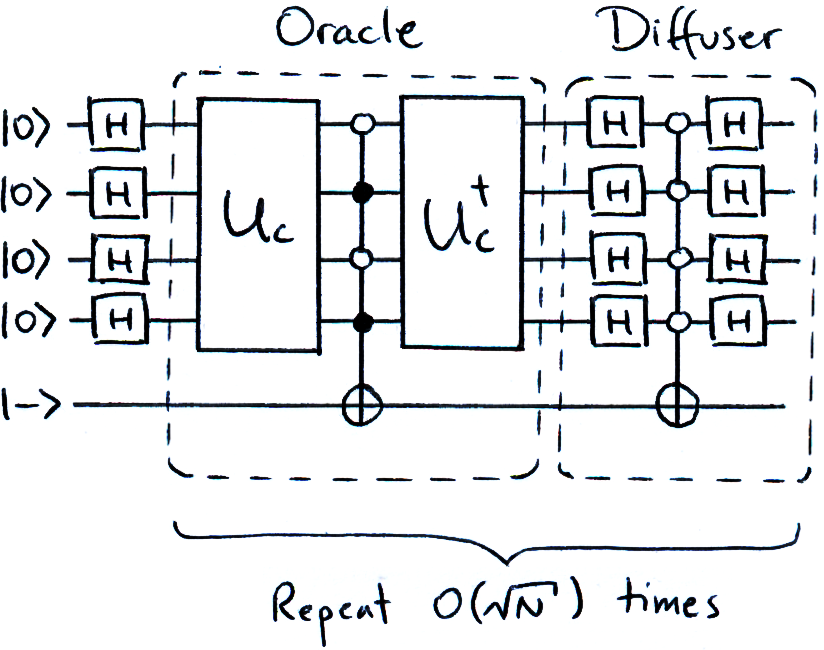
\includegraphics[height= 0.4 \textheight]{figures/grover.png}
    \end{figure}

    Quantum advantage originates from:
    \begin{itemize}
        \item \textbf{Superposition}: Perform an operation to all
        possible solutions at the same time.
        \item \textbf{Interference}: Change sign of the amplitude of the correct solution
        \item \textbf{Entanglement}: Non-trivial sharing of information between states
    \end{itemize}
\end{frame}

\begin{frame}{Important operations}
    \textbf{Welsh-Hadamard transform:} Apply Hadamard gate to every qubit:
    \begin{equation*}
        \textbf{H} \rightarrow \frac{1}{\sqrt{2}}
    \begin{pmatrix}
       1 & 1 \\
       1 & -1  
    \end{pmatrix}
    \end{equation*}

    All possible binary strings with equal amplitude amplitude
    \begin{equation*}
        (- 1)^{\bar{x} \cdot \bar{y}} 2^{- \frac{n}{2}}
    \end{equation*}

    Plus or minus sign depending on the number of ones in the initial and final state
    
    \textbf{Selective face rotation}: Apply a phase to just some specific states.

    \begin{equation*}
        \begin{pmatrix}
            e^{ i \phi_{00}} & 0 & 0 & 0\\
            0 & e^{ i \phi_{01}} & 0 & 0\\
            0 & 0 & e^{ i \phi_{10}} & 0\\
            0 & 0 & 0 & e^{ i \phi_{11}} 
        \end{pmatrix}
    \end{equation*}
    Grover’s algorithm uses this matrix with $\phi_i = \pi$ if the state $i$
    fulfills a condition, and $\phi_j = 0$ otherwise.
\end{frame}

\begin{frame}{Oracle}
    Operator that changes the sign of the amplitudes of the quantum
    states that encode solutions of the problem.

    Common way to change the sign once the solution is detected: 
    \textbf{use an ancillary qubit}.

    Ancilla initialized with an $X$ gate followed by a Hadamard gate:

    \begin{equation*}
        \ket{\psi_a} = HX\ket{0} = H\ket{1} = \frac{1}{\sqrt{2}} (\ket{0} - \ket{1})
    \end{equation*}

    When the $X$ gate is applied:

    \begin{equation*}
        X \ket{\psi_a} = \frac{1}{\sqrt{2}} (\ket{1} - \ket{0}) = - \ket{\psi_a}
    \end{equation*}

    Hint: use CNOT gates to change the sign of the solution. 
\end{frame}

\begin{frame}{Diffusion transform}
    The diffusion transform matrix is a matrix defined as follows:
    \begin{equation}
        D_{ij }=
        \begin{cases}
          \frac{2}{N}, & \text{if}\ i \neq j \\
          - 1 + \frac{2}{N}, & \text{if}\ i = j
        \end{cases}
      \end{equation}

      This can be achieved by applying a Welsh-Hadamard transform on all qubits. Then changing the sign of the $\ket{000 \ldots 000}$
state, and applying once again a Hadamard gate on every qubit.

The diffuser implements an inversion about the average.
\begin{figure}
    \centering
    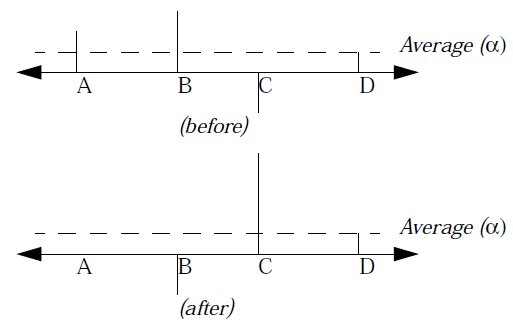
\includegraphics[height= 0.4 \textheight]{figures/inversion.png}
\end{figure}
    
\end{frame}

\begin{frame}{Reason for scaling}
    The quantum state can be understood as a superposition of:
    $$ \ket{\psi_i} = k_i \ket{\Psi_{\text{solution}}} + l_i \ket{\Psi_{\text{not solution}}} $$
    At the start of the algorithm, we can consider $k_0 = \sin \theta$ and $l_0 = \cos \theta $ with $\sin^2 \theta = 1 / N$.

    After the i-th Grover step:
    
    \begin{equation*}
        k_j = \sin (2 j + 1) \theta \quad \text{and} \quad l_j = \frac{1}{\sqrt{N-1}} \cos (2 j + 1) \theta
    \end{equation*}

    \begin{figure}
        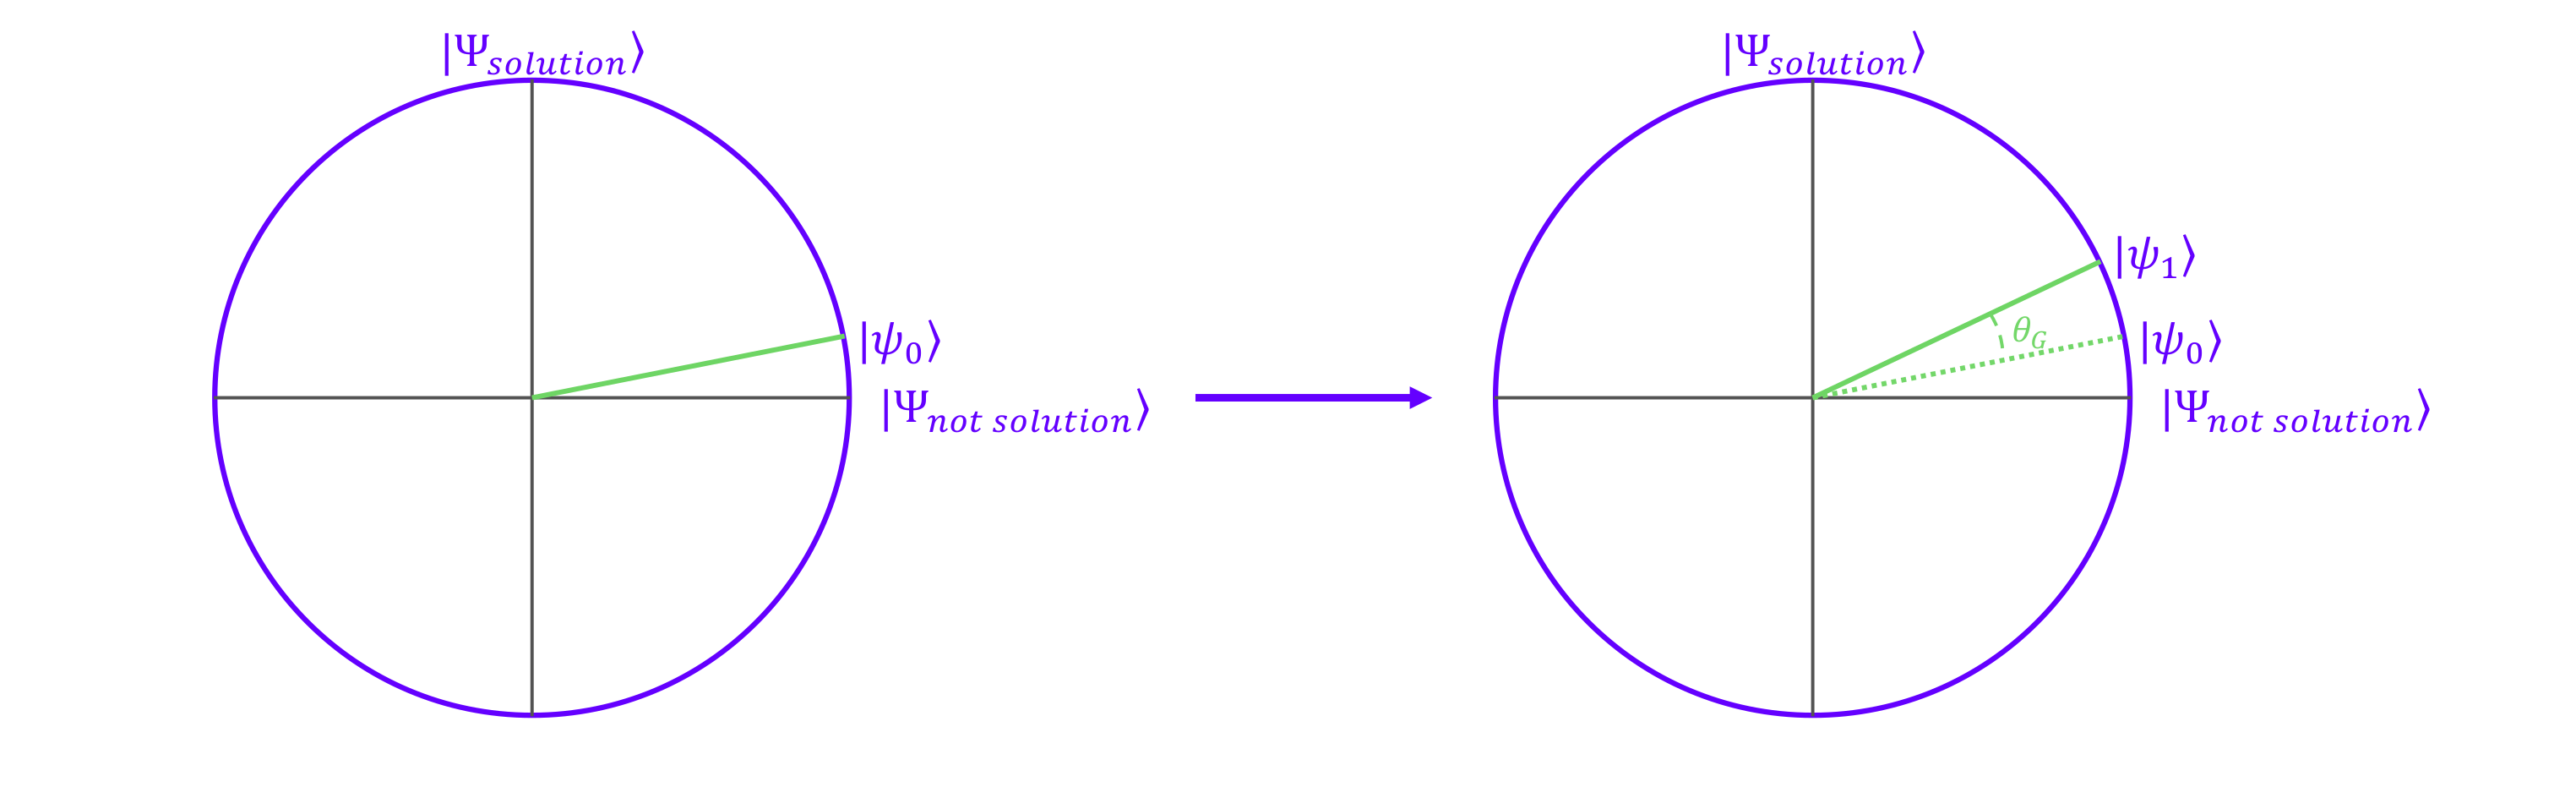
\includegraphics[width= \textwidth]{figures/grover1.png}
    \end{figure}
\end{frame}

\begin{frame}{Reason for scaling}
    \begin{columns}
        \begin{column}{0.5 \textwidth}
            \begin{figure}
                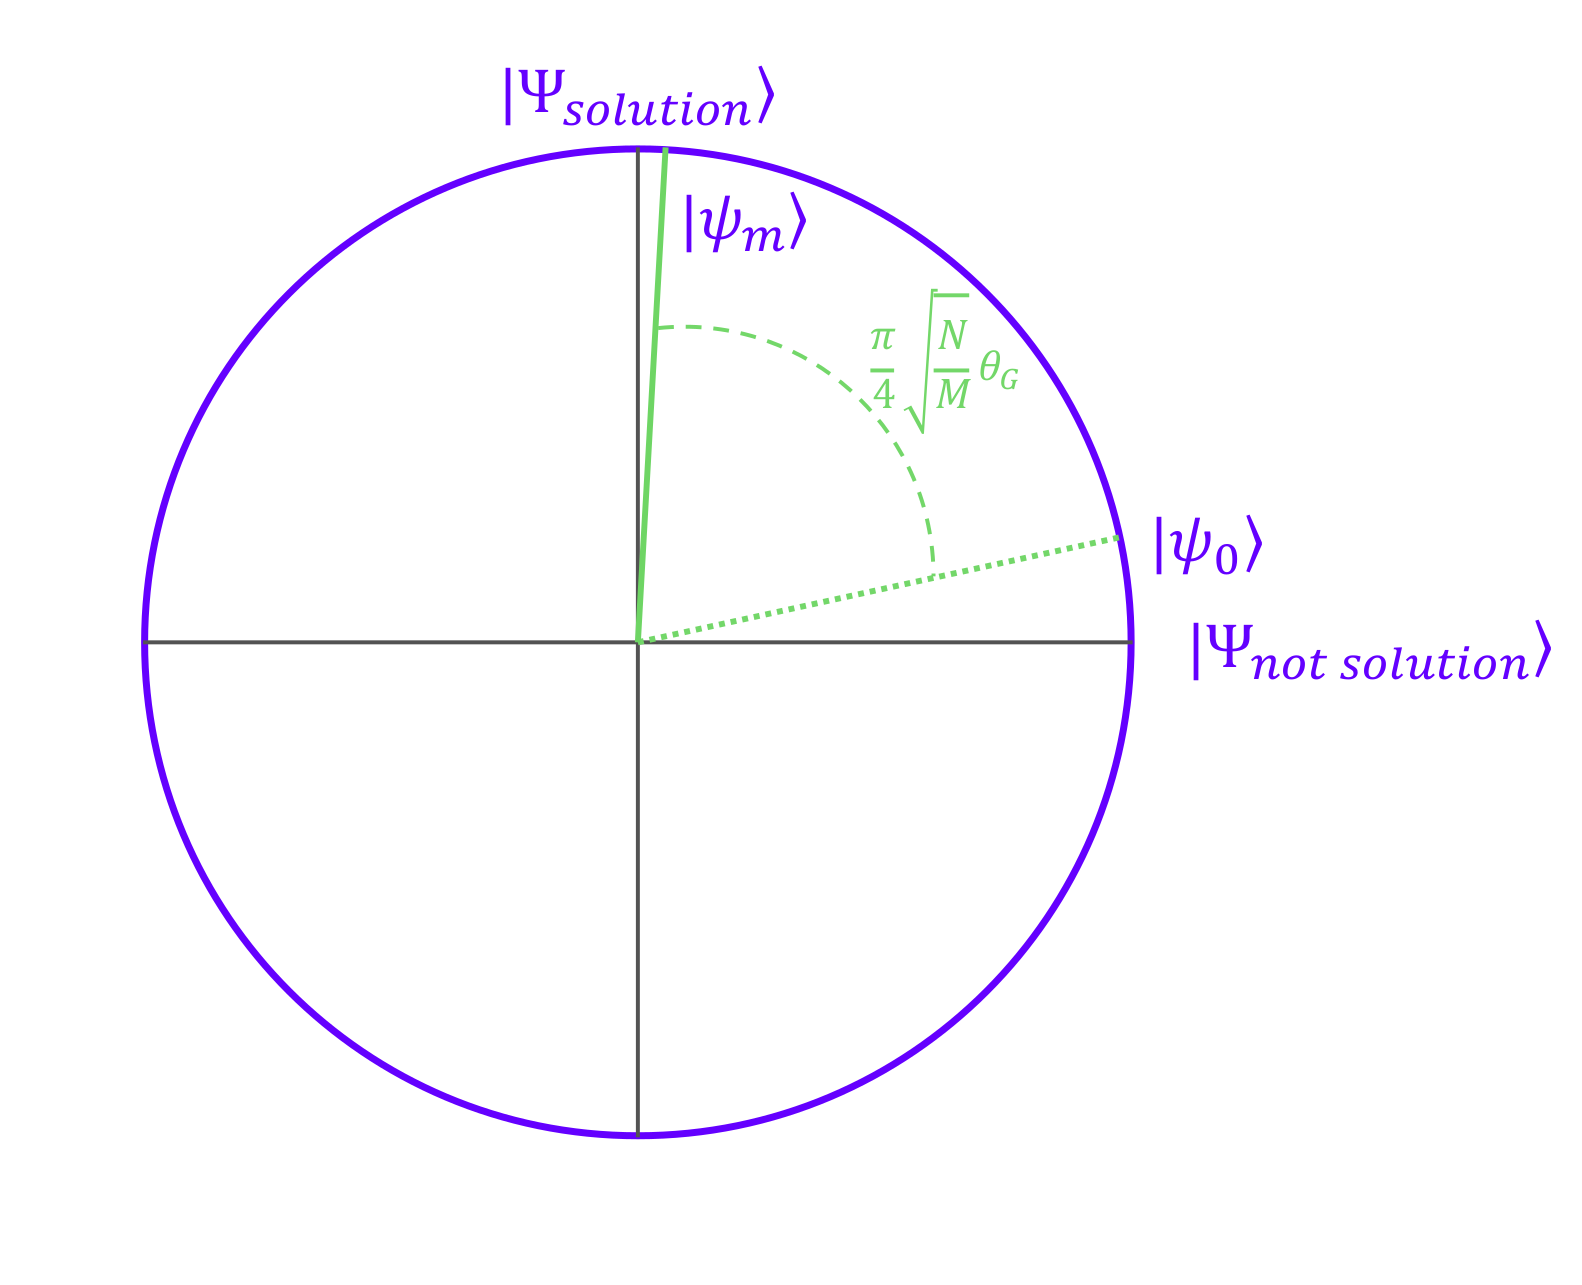
\includegraphics[width= \textwidth]{figures/grover2.png}
            \end{figure}
        \end{column}

        \begin{column}{0.5 \textwidth}
            In order to achieve $k_m = 1$ it follows that $(2 m + 1) \theta = \pi / 2$

    For large number of $N$:

    \begin{equation*}
        \theta \approx \sin \theta = 1 / \sqrt{N}
    \end{equation*}

    The number of iterations needed is the closest integer to

    $$ \frac{\pi}{4} \sqrt{N}$$

    in case of a single solution.

    This can be extended to $ \frac{\pi}{4} \sqrt{\frac{N}{M}}$ when considering
    multiple solutions.
        \end{column}
    \end{columns}
\end{frame}


\section{Outlook}

\begin{frame}{Outlook}
    Qibo is growing to accomodate different tasks:
    \begin{wrapfigure}{r}{0.25\textwidth}
        
\includegraphics[width=0.9\linewidth]{figures/qibo_logo.png} 
        \end{wrapfigure}
    \begin{itemize}
        \item[ \color{teal} \faCheck] High-performance quantum simulation: {\color{blue} \textbf{qibojit}}
        \item[ \color{orange}\faCheck] Hardware control: {\color{red} \textbf{qibolab}}
        \item[ \color{orange} \faCheck] Hardware calibration: { \color{teal} \textbf{qcvv} }
    \end{itemize}

    What makes Qibo different from other libraries:
    \begin{itemize}
        \item[ \faPlus] Public available as an open source project.
        \item[ \faPlus] Modular layout design with possibility of adding
        \begin{itemize}
            \item a new backend for simulation
            \item a new platform for hardware control
        \end{itemize}
        \item[ \faPlus] Community driven effort
    \end{itemize}

    \url{https://github.com/qiboteam/qibo} \hfill \url{https://qibo.readthedocs.io/en/stable/}
\end{frame}
\section{Thanks for listening!}
\end{document}